\documentclass[10pt]{article}
\usepackage{zsj}

\usepackage{silence}
\WarningFilter{latex}{Marginpar on page}

\allowdisplaybreaks

\hbadness=99999

\newcommand{\me}{\mathrm{e}}
%\newcommand{\rr}{\mathbb{R}}
\newcommand{\ii}{\mathrm{i}}
%\newcommand{\md}{\mathrm{d}}
%\DeclareMathOperator{\im}{im}


\usepackage{annotate-equations}
\usepackage{marginfix}
\usepackage{simpler-wick}
\usepackage[export]{adjustbox}

\newenvironment{boxmath}[1]{\begin{tcolorbox}[enhanced,attach boxed title to top center={yshift=-\tcboxedtitleheight/2},boxrule=1pt,title={\centering #1},colframe=NavyBlue!70!black,colback=NavyBlue!10,colbacktitle=NavyBlue!10,fonttitle=\scshape,coltitle=Black]}{\end{tcolorbox}}
\crefname{claim}{claim}{claims}


\begin{document}
\title{Conformal Field Theory}
\subheader{Notes}
\author{Shangjie Zhou\orcidlink{0000-0001-9576-5011}}
\affiliation{School of Physics and Technology, Wuhan University}
\emailAdd{sjzhou@whu.edu.cn}
\abstract{\textit{Last updated on: \today}\\Latest version: \url{https://github.com/spaceofzsj/Conformal-Field-Theory/releases}\\Source files: \url{https://github.com/spaceofzsj/Conformal-Field-Theory}\\Personal Website: \url{https://spaceofzsj.github.io/ShangjieZhou/}}
\maketitle
\phantomsection\addcontentsline{toc}{section}{\protect\numberline{}Introduction}
\section*{Introduction}
A conformal field theory (CFT) is a quantum field theory that is invariant under \textit{conformal transformations}.

Conformal field theory has important applications to condensed matter physics, statistical mechanics, quantum statistical mechanics, and string theory.

This notes are mainly based on the yellow book\cite{DiFrancesco:1997nk}.

There are also useful lecture notes like \cite{Qualls:2015qjb,Tong:2009np}.

\clearpage
\part{Review}
\section{Quantum Field Theory}
This section only contains some topics of QFT and necessary notations we will use later.
For a complete introduction to QFT, see \cite{Peskin:1995ev,srednicki_2007,weinberg_1995,schwartz_2013,Zee:2003mt,Coleman:2018mew}.
\subsection{Path Integral Quantization}
\begin{intu}
    The way to quantize a \textit{classical} system\mn{Geometric quantization is among them\cite{woodhouse1997geometric,carosso2018geometric}. See more about this topic in \cite{Ali:2004ft}.} is not unique and different formulations of quantization may give different results.
    For example, in canonical quantization, the ordering of operators may lead to different quantization \textit{schemes}.
    Different quantization formulations may have mathematical connections which may simplify problems.
    
    In each quantization formalism, the method to compute the correlation function of fields must be given and the results of correlation functions are used to judge if the formalisms are equivalent.
\end{intu}
In the path integral formulation of QFT, we directly\sidenote{In canonical quantization, we do not directly compute the correlation function. Instead, we first construct Hilbert space and opertors in it.} focus on correlation functions of fields.
\subsubsection{Lorentzian Formalism}
In a Lorentzian spacetime, we define the Lorentzian quantization of field by requiring the correlation functions to satisfy the following relation:
\begin{boxmath}{Lorentzian Path Integral Quantization}
    \begin{align}
        \expval{\phi_1(x_1)\dots\phi_n(x_n)}=\frac{\int [\dd[]{\phi}]\phi_1(x_1)\dots\phi_n(x_n)\exp(\ii S[\phi])}{\int[\dd[]{\phi}]\exp(\ii S[\phi])}
    \end{align}
\end{boxmath}
where the time integral of the action $S=\int\dd[4]{x}\mathcal{L}$ should be performed along $t(1-\ii\epsilon)$ where $\epsilon\to0$ (see \cite{Peskin:1995ev} for more details).
\subsubsection{Euclidean Formalism}
In a Euclidean spacetime, there is no notion of "time", so we simply pick out a coordinate and call it "Euclidean time" $\tau$.
We define the Euclidean quantization of field by requiring the correlation functions to satisfy the following relation:
\begin{boxmath}{Euclidean Path Integral Quantization}
    \begin{align}
        \expval{\phi_1(\tau_1,\vec{x}_1)\dots\phi_n(\tau_n,\vec{x}_n)}=\frac{\int [\dd[]{\phi}]\phi_1(\tau_1,\vec{x}_1)\dots\phi_n(\tau_n,\vec{x}_n)\exp(-S_E[\phi])}{\int [\dd[]{\phi}]\exp(-S_E[\phi])}
    \end{align}
\end{boxmath}
\subsubsection{Lorentzian/Euclidean Duality}
\subsection{Symmetries and Conservation Laws}
\subsubsection{Continuous Symmetry Transformations}
Consider a collection of fields, which are denoted by $\Phi(x)$.
The action is
\begin{align}
    S=\int\dd[d]{x}\mathcal{L}\left(\Phi,\partial_\mu\Phi\right).
\end{align}
Consider a transformation affecting both the position and the field
\begin{subequations}\label{eq:CST:transformations}
    \begin{align}
        x       & \to x'       \\
        \Phi(x) & \to\Phi'(x')
    \end{align}
\end{subequations}
In the transformations \cref{eq:CST:transformations}, the new field $\Phi'$ at $x'$ is expressed as a function of the old field $\Phi$ at $x$
\begin{align}
    \Phi'(x')=\mathcal{F}\left[\Phi(x)\right].
\end{align}
\begin{figure}[h]
    \centering
    \includegraphics[width=0.5\linewidth]{fig/Quantum Field Theory/transformation_illustration/fig.pdf}
    \caption{A illustration of the transformation of the fields where the background spacetime is 2-dimensional. The colored areas are the non-vanishing part of the fields.}
\end{figure}

The new action is
\begin{align}
    S' & =\int\dd[d]{x}\mathcal{L}\left(\Phi'(x),\partial_\mu\Phi'(x)\right)\notag                                                                                               \\
       & =\int\dd[d]{x'}\mathcal{L}\left(\Phi'(x'),\partial'_\mu\Phi'(x')\right)\notag                                                                                           \\
       & =\int\dd[d]{x'}\mathcal{L}\left(\mathcal{F}\left[\Phi(x)\right],\partial'_\mu\mathcal{F}\left[\Phi(x)\right]\right)\notag                                               \\
       & =\int\dd[d]{x}\abs{\pdv{x'}{x}}\mathcal{L}\left(\mathcal{F}[\Phi(x)],\left(\pdv*{x^\nu}{x'^\mu}\right)\partial_\nu\mathcal{F}[\Phi(x)]\right).\label{eq:CST:new_action}
\end{align}
\subsubsection{Infinitesimal Transformations and Noether's Theorem}
Infinitesimal transformations may in general written as\sidenote{We often denote $\mathcal{F}[\phi(x)]$ by $\mathcal{F}(x)$.}
\begin{align}
    x'^\mu    & =x^\mu+\omega_a\fdv{x^\mu}{\omega_a}\label{eq:CST:x_prime}               \\
    \Phi'(x') & =\Phi(x)+\omega_a \fdv{\mathcal{F}(x)}{\omega_a}\label{eq:CST:phi_prime}
\end{align}
Here $\{\omega_a\}$ is a set of infinitesimal parameters, which will be kept to first order only.
\begin{definition}[Generator of a symmetry transformation]\label{def:generator_of_a_symmetry_transformation}
    The \textit{generator} $G_a$ of a symmetry transformation is defined by the following expression for the infinitesimal transformation at a same point:
    \begin{align}
        \delta_\omega\Phi(x)\equiv\Phi'(x)-\Phi(x)\equiv-\ii\omega_a G_a\Phi(x).
    \end{align}
\end{definition}
Notice that
\begin{align}
    \Phi'(x')=\Phi(x)+\omega_a \fdv{\mathcal{F}(x)}{\omega_a}=\Phi(x')-\omega_a\fdv{x^\mu}{\omega_a}\partial_\mu\Phi(x')+\omega_a\fdv{\mathcal{F}(x')}{\omega_a}
\end{align}
The explicit expression of the generator is therefore
\begin{align}
    \ii G_a\Phi=\fdv{x^\mu}{\omega_a}\partial_\mu\Phi-\fdv{\mathcal{F}}{\omega_a}\label{eq:CST:explicit_generator}
\end{align}
\begin{example}[Infinitesimal translation]
    For an infinitesimal translation by a vector $\omega_\mu$, one has $\fdv*{x^\mu}{\omega^\nu}=\delta^\mu_\nu$ and $\fdv*{\mathcal{F}}{\omega^\nu}=0$.
    The generator of translations is simply
    \begin{align}
        P_\nu=-\ii\partial_\nu.\label{eq:CST:translation_operator}
    \end{align}
\end{example}
\begin{example}[Infinitesimal Lorentz transformation]
    An infinitesimal Lorentz transformation has the form
    \begin{align}
        x'^\mu=x^\mu+\tensor{\omega}{^\mu_\nu}x^\nu=x^\mu+\omega_{\rho\nu}\eta^{\rho\mu}x^\nu.
    \end{align}
    where $\omega_{\rho\nu}=-\omega_{\nu\rho}$.
    Thus the variation of coordinates under transformation is
    \begin{align}
        \fdv{x^\mu}{\omega_{\rho\nu}}=\frac{1}{2}\left(\eta^{\rho\mu}x^\nu-\eta^{\nu\mu}x^\rho\right).\label{eq:CST:lorentz_x}
    \end{align}
    And its effect on the generic field $\Phi$ is
    \begin{align}
        \mathcal{F}[\Phi]=L_\Lambda \Phi\qq{and}L_\Lambda\approx1-\frac{1}{2}\ii\omega_{\rho\nu}S^{\rho\nu}\label{eq:CST:lorentz_phi}
    \end{align}
    where  $S^{\rho\nu}$ is some Hermitian matrix obeying the Lorentz algebra.
    Using \cref{eq:CST:explicit_generator}, we have
    \begin{align}
        \frac{1}{2}\ii\omega_{\rho\nu}L^{\rho\nu}\Phi=\frac{1}{2}\omega_{\rho\nu}\left(x^\nu\partial^\rho-x^\rho\partial^\nu\right)\Phi+\frac{1}{2}\ii\omega_{\rho\nu}S^{\rho\nu}\Phi
    \end{align}
    The generators of the Lorentz transformation are thus
    \begin{align}
        L^{\rho\nu}=\ii\left(x^\rho\partial^{\nu}-x^\nu\partial^\rho\right)+S^{\rho\nu}.\label{eq:CST:Lorentz_operator}
    \end{align}
\end{example}
\begin{theorem}[Noether's theorem]
    Every continuous symmetry of the action is associated with a current that is \textit{classically}\mn{Notice the \textit{classically}. In the quantum case, it may happen that the path integration measure does not possess the symmetry of the action, in which case that symmetry is said to be \textit{anomalous}.} conserved.
\end{theorem}
\begin{proof}
    Using \cref{eq:CST:x_prime,eq:CST:phi_prime} in \cref{eq:CST:new_action}, we have
    \begin{align}
        \pdv{x'^\mu}{x^\mu}=\delta^\nu_\mu+\partial_\mu\left(\omega_a\fdv{x^\nu}{\omega_a}\right).\label{eq:qft:infinitesimal_inverse}
    \end{align}
    Using the first order approximation of the determinant of a matrix
    \begin{align}
        \det(1+E)\approx1+\Tr E\quad(E\ \text{is small})
    \end{align}
    we have
    \begin{align}
        \abs{\pdv{x'}{x}}\approx1+\partial_\mu\left(\omega_a\fdv{x^\mu}{\omega}\right)
    \end{align}
    and the reverse of \cref{eq:qft:infinitesimal_inverse} is
    \begin{align}
        \pdv{x^\nu}{x'^\mu}=\delta^\nu_\mu-\partial_\mu\left(\omega_a\fdv{x^\nu}{\omega_a}\right).
    \end{align}
    Now \cref{eq:CST:new_action} becomes
    \begin{align}
        S'= & \int\dd[d]{x}\left(1+\partial_\mu\left(\omega_a\fdv{x^\mu}{\omega_a}\right)\right)\notag                                                                                                                                                             \\
            & \times\mathcal{L}\left(\Phi+\omega_a\fdv{\mathcal{F}}{\omega_a},\left[\delta^\nu_\mu-\partial_\mu\left(\omega_a\fdv{x^\nu}{\omega_a}\right)\right]\left[\partial_\nu\Phi+\partial_\nu\left(\omega_a\fdv{\mathcal{F}}{\omega_a}\right)\right]\right).
    \end{align}
    From the definition of symmetry, when $\omega_a$ are constants the variation $\delta S$ vanishes.
    So $\delta S$ can only contain first derivatives of $\omega_a$, obtained by expanding the Lagrangian\mn{This is where the symmetry condition is used: when the transformation is not a symmetry transformation, if $\omega_a$ is constant then $\delta S$ may not vanish, and the expansion must involve terms without derivative; when the transformation is a symmetry transformation, if $\omega_a$ is constant then $\delta S=0$, so it is reasonable there are only terms with derivatives in $\delta S$ and all the terms without derivatives must sum up to $0$. After expanding $\delta S$, we find that that there is only term with first derivative.},
    \begin{align}
        \delta S\equiv S'-S=-\int\dd[d]{x}j^\mu_a\partial_\mu\omega_a\label{eq:nother:before_integration}
    \end{align}
    where
    \begin{align}
        j^\mu_a\equiv\left(\pdv{\mathcal{L}}{(\partial_\mu\Phi)}\partial_\nu\Phi-\delta^\mu_\nu\mathcal{L}\right)\fdv{x^\nu}{\omega_a}-\pdv{\mathcal{L}}{(\partial_\mu\Phi)}\fdv{\mathcal{F}}{\omega_a}.\label{eq:nother:canonical_current}
    \end{align}
    $j^\mu_a$ is called the \textit{current} associated with the infinitesimal transformation.
    Integrate \cref{eq:nother:before_integration} by parts
    \begin{align}
        \delta S=\int\dd[d]{x}\partial_\mu j^\mu_a \omega_a.
    \end{align}
    When the field configuration obeys the classical equation of motion, $\delta S=0$ for any postion-dependent parameters $\omega_a(x)$, which implies the conservation law
    \begin{align}
        \partial_\mu j^\mu_a=0.
    \end{align}
    The conserved charge associated with $j^\mu_a$ is
    \begin{align}
        Q_a\equiv\int\dd[d-1]{x}j^0_a.
    \end{align}
    We can show that
    \begin{align}
        \dot{Q}_a= & \int\dd[d-1]{x}\partial_0 j^0_a\notag                            \\
        =          & -\int\dd[d-1]{x}\partial_i j^i_a\label{eq:nother:stocks_theorem} \\
        =          & -\int_\infty j^i_a\dd{\sigma^i}\notag                            \\
        =          & 0
    \end{align}
    where we used Stokes' theorem in \cref{eq:nother:stocks_theorem} and $\dd{\sigma^i}$ is the turface element at spatial infinity.
\end{proof}
\begin{remark}
    We can freely add $j^\mu_a$ the divergence of an antisymmetric tensor without affecting the conservation
    \begin{align}
        j^\mu_a\to j^\mu_a+\partial_\nu B^{\nu\mu}_a\qq{where} B^{\nu\mu}_a=-B^{\mu\nu}_a\label{eq:nother:equiv_current}
    \end{align}
    since $\partial_\mu\partial_\nu B^{\nu\mu}_a=0$ by antisymmetry.
    The current we defined in \cref{eq:nother:canonical_current} is said to be \textit{canonical}.
\end{remark}
\subsubsection{Transformations of the Correlation Functions}
Consider the general correlation function
\begin{align}
    \expval{\Phi(x_1)\dots\Phi(x_n)}=\frac{1}{\eqnmarkbox[blue]{node1}{Z}}\int\left[\dd{\Phi}\right]\Phi(x_1)\dots\Phi(x_n)\exp(-\eqnmarkbox[purple]{node2}{S[\Phi]})
\end{align}
\annotate[yshift=-0.1em]{below}{node1}{Vacuum functional}
\annotate[yshift=0.5em]{}{node2}{Euclidean action}

When the transformation \cref{eq:CST:transformations} is a symmetry, we have the following constraint on the correlation function
\begin{subequations}\label{eq:TCF:correlation_transform}
    \begin{align}
        \expval{\Phi(x_1')\dots\Phi(x_n')}= & \frac{1}{Z}\int\left[\dd{\Phi}\right]\Phi(x_1')\dots\Phi(x_n')\exp(-S(\Phi))\notag                                                                  \\
        =                                   & \frac{1}{Z}\int\left[\dd{\Phi'}\right]\Phi'(x_1')\dots\Phi'(x_n')\exp(-S(\Phi'))\label{eq:TCF:measure1}                                             \\
        =                                   & \frac{1}{Z}\int\left[\dd{\Phi}\right]\mathcal{F}\left(\Phi(x_1')\right)\dots\mathcal{F}\left(\Phi(x_n')\right)\exp(-S(\Phi))\label{eq:TCF:measure2} \\
        =                                   & \expval{\mathcal{F}\left(\Phi(x_1)\right)\dots\mathcal{F}\left(\Phi(x_n)\right)}
    \end{align}
\end{subequations}
We have assumed the Jacobian of this change of variable is trivial in \crefrange{eq:TCF:measure1}{eq:TCF:measure2}\sidenote{This is in fact the main obstacle to conformal invariance in a quantum symmetry: the action may well be scale invariant, but the measure is not because of the regularization procedure needed to define it properly.}.

\subsubsection{Ward Identities}
We can write the \textit{global} infinitesimal transformation as

\begin{align}
    \Phi'(x)=\Phi(x)-\ii\eqnmarkbox[blue]{node1}{\omega_a} G_a\Phi(x).
\end{align}\annotate[yshift=0.5em]{}{node1}{Infinitesimal constant parameters}

Now we consider the \textit{local} infinitesimal transformation in which parameters will depend on spacetime coordinates
\begin{align}
    \Phi'(x)=\Phi(x)-\ii\omega_a(x) G_a\Phi(x).
\end{align}
Denoting by $X$ and $X'$ the collection $\Phi(x_1)\dots\Phi(x_n)$ and $\Phi'(x_1)\dots\Phi'(x_n)$ of fields in the correlation function respectively and by $\delta_\omega X\equiv X'-X$ its variation under the transformation, we can do a change of variable
\begin{align}
    \expval{X}= & \frac{1}{Z}\int\left[\dd{\Phi}\right]X\exp(-S[\Phi])\notag                                                                                                                       \\
    =           & \frac{1}{Z}\int\left[\dd{\Phi'}\right]X'\exp(-S[\Phi'])\notag                                                                                                                    \\
    =           & \frac{1}{Z}\int\left[\dd{\Phi}\right]\left(X+\delta_\omega X\right)\exp\left[-\left(S[\Phi]+\int\dd[d]{x}\partial_\mu j^\mu_a\omega_a(x)\right)\right]\label{eq:ward:before_est}
\end{align}
where we have used \cref{eq:nother:before_integration} and assuemd the functional integration measure is invariant under the transformation $\left[\dd{\Phi'}\right]=\left[\dd[]{\Phi}\right]$.
Expand \cref{eq:ward:before_est} to first order in $\omega_a(x)$, we have
\begin{align}
    \expval{X} & =\frac{1}{Z}\int\left[\dd[]{\Phi}\right]\left(X+\delta_\omega X\right)\exp(-S)\left[1-\int\dd[]{x}\partial_\mu j^\mu_a\omega_a(x)\right]\notag \\
               & =\expval{X}+\expval{\delta_\omega X}-\int\dd[d]{x}\partial_\mu\expval{j^\mu_a(x)X}\omega_a(x)
\end{align}
which finally gives\sidenote{It is clearly that $$\expval{\delta_\omega X}=\delta_\omega\expval{X}.$$}
\begin{align}
    \expval{\delta_\omega X}=\int\dd[d]{x}\partial_\mu\expval{j^\mu_a(x)X}\omega_a(x).\label{eq:ward:anyomega}
\end{align}
The variation $\delta_\omega X$ is explicitly given to first order in $\omega_a(x)$ by
\begin{align}
    \delta_\omega X & =-\ii\sum_{i=1}^n\left(\Phi(x_1)\dots G_a\Phi(x_i)\dots\Phi(x_n)\right)\omega_a(x_i)\notag                    \\
                    & =-\ii\int\dd[d]{x}\omega_a(x)\sum_{i=1}^n\left[\Phi(x_1)\dots G_a\Phi(x_i)\dots\Phi(x_n)\right]\delta(x-x_i).
\end{align}
Since \cref{eq:ward:anyomega} holds for any $\omega_a(x)$, we have the local relation which is called the \textit{Ward identity} for the current $j^\mu_a$.
\begin{boxmath}{Ward Identity}
    \begin{align}
        \pdv{x^\mu}\expval{j^\mu_a(x)\Phi(x_1)\dots\Phi(x_n)}=-\ii\sum^n_{i=1}\delta(x-x_i)\expval{\Phi(x_1)\dots G_a\Phi(x_i)\dots\Phi(x_n)}.\label{eq:QFT:ward_identity}
    \end{align}
\end{boxmath}
\begin{remark}
    The form of the current may be modified from the canonical definition \cref{eq:nother:canonical_current} without affecting the Ward identity, if we add a term to $j^\mu_a$ that is divergenceless identically.
\end{remark}
\subsection{The Energy-Momentum Tensor}
The conserved current associated with translation invariance is the \textit{energy-momentum tensor}, whose components are the density and flux density of energy and momentum.

Consider the infinitesimal translation\sidenote{The field is unaffected by the translation.} $x^\mu\to x^\mu+\epsilon^\mu$, we have
\begin{align}
    \fdv{x^\mu}{\epsilon^\nu}=\delta^\mu_\nu\quad\fdv{\mathcal{F}[\Phi]}{\epsilon^\mu}=0.
\end{align}
Using \cref{eq:nother:canonical_current}, the corresponding canonical conserved current is
\begin{align}
    T^{\mu\nu}_c\equiv-\eta^{\mu\nu}\mathcal{L}+\pdv{\mathcal{L}}{(\partial_\mu\Phi)}\partial^\nu\Phi
\end{align}
which satisfies
\begin{align}
    \partial_\mu T^{\mu\nu}_c=0.
\end{align}
The conserved charge is the 4-momentum
\begin{align}
    P^\nu\equiv\int\dd[d-1]{x}T^{0\nu}_c.
\end{align}
In particular, the energy is
\begin{align}
    P^0=\int\dd[d-1]{x}\left(\pdv{\mathcal{L}}{\dot{\Phi}}\dot{\Phi}-\mathcal{L}\right)
\end{align}
which is the usual definition of the Hamiltonian.

\subsubsection{The Belinfante Tensor\label{subsubsec:The_Belinfante_Tensor}}
\begin{intu}
    In general, the canonical energy-momentum operator is not symmetric, we can make it symmetric \textit{classically} by adding $T^{\mu\nu}_c$ an divergenceless term without breaking the conservation law or the Ward identity
    \begin{align}
        T^{\mu\nu}_B\equiv T^{\mu\nu}_c+\partial_{\rho}B^{\rho\mu\nu}\qq{where}B^{\rho\mu\nu}=-B^{\mu\rho\nu}.\label{eq:Belinfante:def}
    \end{align}
\end{intu}
The variation of the action under a nonuniform translation with position-dependent parameter $\epsilon^\mu(x)$ is still
\begin{align}
    \delta S=\int\dd[d]{x}\partial_\mu T^{\mu\nu}_B\epsilon_\nu
\end{align}
since $\partial_\mu T^{\mu\nu}_B=\partial_\mu T^{\mu\nu}_c$.

If we succeed in finding $B^{\rho\mu\nu}$ such that the new tensor $T^{\mu\nu}_B$ is symmetric, then the latter is called the \textit{Belinfante} energy-momentum tensor.

\paragraph{Finding Belinfante tensor}
From \cref{eq:CST:lorentz_x,eq:CST:lorentz_phi}, under infinitesimal Lorentz transformation, the coordinates and fields change as
\begin{align}
    \fdv{x^\rho}{\omega_{\mu\nu}}=\frac{1}{2}\left(\eta^{\rho\mu}x^\nu-\eta^{\rho\nu}x^\mu\right)\qand\fdv{\mathcal{F}}{\omega_{\mu\nu}}=-\frac{\ii}{2}S^{\mu\nu}\rho
\end{align}
and the associated conserved current is
\begin{align}
    j^{\mu\nu\rho}=T^{\mu\nu}_c x^\rho-T^{\mu\rho}_c x^\nu+\ii\pdv{\mathcal{L}}{(\partial_\mu\Phi)}S^{\nu\rho}\Phi.\label{eq:Belinfante:lorentz_current}
\end{align}
\begin{claim}
    One of the possible form of $B^{\rho\mu\nu}$ that will make $T^{\mu\nu}_B$ symmetric is
    \begin{align}
        B^{\mu\rho\nu}=\frac{\ii}{2}\left[\pdv{\mathcal{L}}{(\partial_\mu\Phi)}S^{\nu\rho}\Phi+\pdv{\mathcal{L}}{(\partial_\rho\Phi)}S^{\mu\nu}\Phi+\pdv{\mathcal{L}}{(\partial_\nu\Phi)}S^{\mu\rho}\Phi\right].\label{eq:Belinfante:B}
    \end{align}
\end{claim}
\begin{proof}
    Using the fact $S^{\mu\nu}=-S^{\nu\mu}$, it can be easily checked that $B^{\mu\rho\nu}=-B^{\rho\mu\nu}$.
    
    We can explicitly show that
    \begin{align}
        B^{\mu\rho\nu}-B^{\mu\nu\rho}=\ii\pdv{\mathcal{L}}{(\partial_\mu\Phi)}S^{\nu\rho}\Phi.
    \end{align}
    Acting $\partial_\mu$ on both sides of \cref{eq:Belinfante:lorentz_current}, we have
    \begin{align}
        T^{\rho\nu}_c-T^{\nu\rho}_c=-\ii\partial_\mu\left[\pdv{\mathcal{L}}{(\partial_\mu\Phi)}S^{\nu\rho}\Phi\right]
    \end{align}
    where the conservation laws $\partial_\mu j^{\mu\nu\rho}=0$ and $\partial_\mu T^{\mu\nu}=0$ are used.
    We see that the antisymmetric part of $T^{\rho\nu}_c+\partial_\mu B^{\mu\rho\nu}$ vanishes which means $T^{\mu\nu}_B$ is indeed symmetric \textit{in a classical configuration}\mn{The symmetry is not guaranteed in any configuration, namely not \textit{identically}.}.
\end{proof}
\begin{remark}
    The form of $B^{\mu\rho\nu}$ is not unique.
    We use \cref{eq:Belinfante:B} to define $T_B^{\mu\nu}$ in this note.
    
    Notice that the Belinfante tensor can only be defined in a theory with Lorentz invariance and is only symmetric classically.
    
    And with $T^{\mu\nu}_B$ we can write the conserved current for Lorentz symmetry as\mn{Check it! It differs from the conserved current in \cref{eq:Belinfante:lorentz_current} by a divergenceless term which means they are equivalent.}
    \begin{align}
        j^{\mu\nu\rho}=T^{\mu\nu}_B x^\rho-T^{\mu\rho}_B x^\nu.\label{eq:Belinfante:after_stress_tensor}
    \end{align}
\end{remark}
\begin{example}[Massive vector field\label{ex:massive_vector_field}]
    Consider the following Lagrangian for a massive vector field $A_\mu$ (in Euclidean spacetime)
    \begin{align}
        \mathcal{L}=\frac{1}{4}F^{\alpha\beta}F_{\alpha\beta}+\frac{1}{2}m^2 A^\alpha A_\alpha
    \end{align}
    where $F_{\alpha\beta}\equiv\partial_\alpha A_\beta-\partial_\beta A_\alpha$.
    The canonical energy-momentum tensor is
    \begin{align}
        T^{\mu\nu}_c=F^{\mu\alpha}\partial^\nu A_\alpha-\eta^{\mu\nu}\mathcal{L}
    \end{align}
    which is not symmetric.
    Using \cref{eq:Belinfante:B,eq:Belinfante:def}, we have
    \begin{align}
        B^{\alpha\mu\nu}= & F^{\alpha\mu}A^\nu                                                                 \\
        T^{\mu\nu}_B=     & T^{\mu\nu}_c+F^{\alpha\mu}\partial_\alpha A^\nu+\partial_\alpha F^{\alpha\mu}A^\nu
    \end{align}
    and we know $T^{\mu\nu}_B$ is classically symmetric.
\end{example}
\begin{intu}
    Although we can replace the canonical energy-momentum tensor $T^{\mu\nu}_c$ by Belinfante tensor $T^{\mu\nu}_B$ without breaking the Ward identity, the $T^{\mu\nu}_B$ in Ward identity is not symmetric\mn{$T^{\mu\nu}_B$ is symmetric classically and in Ward identity we consider all possible field configuration.}.
    
    In fact, it is possible to define a new energy-momentum tensor $\tilde{T}^{\mu\nu}_B$ which is a conserved current classically and symmetric in any field configuration, namely \textit{identically} symmetric.
    And in general\mn[2em]{So not in every case.} we can directly substitute $\tilde{T}^{\mu\nu}_B$ into the Ward identity for $T^{\mu\nu}_c$ without breaking it.
\end{intu}
In \cref{ex:massive_vector_field}, we may define
\begin{align}
    \tilde{T}^{\mu\nu}_B\equiv T^{\mu\nu}_B-\left(\partial_\alpha F^{\alpha\mu}-m^2 A^\mu\right)A^\nu.
\end{align}
We have $\tilde{T}^{\mu\nu}_B=T^{\mu\nu}_B$ classically using equation of motion and $\tilde{T}^{\mu\nu}_B$ can be directly used to replace $T^{\mu\nu}_c$ in the Ward identity for translation (see \cite{DiFrancesco:1997nk} for details\sidenote{\label{sidenote:modified_EM_tensor}The idea is that if we use the modified energy-momentum tensor $\tilde{T}^{\mu\nu}_B$, there will be an extra divergence term in the LHS of Ward identity \cref{eq:QFT:ward_identity}. Since the Dirac delta function has a precise meaning only after integration over some volume, we often integrate the Ward identity for furthur use and after the integration, the divergence term will vanish as a surface term.}).
\subsubsection{Hilbert Energy-Momentum Tensor}
Consider an infinitesimal translation of the coordinates $x^\mu\to x^\mu+\epsilon^\mu(x)$.
The variation of the action $\delta S$ can be calculated using \cref{eq:nother:before_integration}.
We want to define a new energy momentum tensor $\Theta^{\mu\nu}$ which satisfies
\begin{align}
    \delta S\equiv-\frac{1}{2}\int\dd[d]{x}\Theta^{\mu\nu}\left(\partial_\mu\epsilon_\nu+\partial_\nu\epsilon_\mu\right)\label{eq:alternate_tensor:requirement}
\end{align}

%According to \cref{eq:nother:before_integration}, we have
%\begin{align}
%    \delta S= & \int\dd[d]{x}T^{\mu\nu}\partial_\mu\epsilon_\nu\notag                                                                               \\
%    =         & \frac{1}{2}\int\dd[d]{x}T^{\mu\nu}\left(\partial_\mu\epsilon_\nu+\partial_\nu\epsilon_\mu\right)\label{eq:alternate_tensor:delta_s}
%\end{align}
%where we have used identically symmetric energy-momentum tensor $T^{\mu\nu}$\sidenote{\Cref{eq:nother:before_integration} is actually valid for $T^{\mu\nu}_B$. The reason that it works when we use $T^{\mu\nu}$ instead of $T^{\mu\nu}_B$ is discussed in the Physics Stack Exchange questions \url{https://physics.stackexchange.com/q/119838} (version: 2014-06-18) and \url{https://physics.stackexchange.com/q/270877} (version: 2016-08-06)}.

%The induced metric of the map $x^\mu\to x'^\mu+\epsilon^\mu(x)$ to first order in $\epsilon$ is
%\begin{align}
%    g'_{\mu\nu}= & \pdv{x^\alpha}{x'^\mu}\pdv{x^\beta}{x'^\nu}g_{\alpha\beta}\notag                                                                   \\
%    =            & \left(\delta^\alpha_\mu-\partial_\mu\epsilon^\alpha\right)\left(\delta^\beta_\nu-\partial_\nu\epsilon^\beta\right)g_{\alpha\beta}.\notag\\
%    =&g_{\mu\nu}-\left(\partial_\mu\epsilon_\nu+\partial_\nu\epsilon_\mu\right)
%\end{align}
%and so 
%\begin{align}
%    \delta g_{\mu\nu}\equiv g'_{\mu\nu}-g_{\mu\nu}=-\left(\partial_\mu\epsilon_\nu+\partial_\nu\epsilon_\mu\right).
%\end{align}
%\begin{intu}
%    The form of the variation of the metric is a hint of a new definition of the energy-momentum tensor.
%    We can rewrite \cref{eq:alternate_tensor:delta_s}
%    \begin{align}
%        \delta S=-\frac{1}{2}\int\dd[d]{x}T^{\mu\nu}\delta g_{\mu\nu}.
%    \end{align}
%\end{intu}
\begin{definition}[Hilbert energy-momentum tensor\label{def:alternate_energy_momentum}]
    The Hilbert energy-momentum tensor $\Theta^{\mu\nu}$ is defined to be proportional to the functional derivative of the action with respect to the metric, evaluated in flat space:
    \begin{align}
        \Theta^{\mu\nu}\equiv-2\eval{\fdv{S}{g_{\mu\nu}}}_{g_{\mu\nu}=\eta_{\mu\nu}}\label{eq:alternate_tensor:equation}
    \end{align}
    where the field is fixed and the background geometry is varied.
    We have coupled the original theory to gravity which means we have to do the \textit{minimal coupling}\mn{Replace the partial derivatives by covariant derivatives and flat metric by a general metric in $S$.}.
\end{definition}
\begin{claim}
    The new energy-momentum tensor $\Theta^{\mu\nu}$ in \cref{def:alternate_energy_momentum} satisfies \cref{eq:alternate_tensor:requirement}.
\end{claim}
\begin{proof}
    The diffeomorphism $x^\mu\to x^\mu+\epsilon^\mu(x)$ will induce a new metric $g'_{\mu\nu}$ and the variation of metric can be shown to be
    \begin{align}
        \delta g_{\mu\nu}\equiv g'_{\mu\nu}-g_{\mu\nu}=-\left(\partial_\mu\epsilon_\nu+\partial_\nu\epsilon_\mu\right)\label{eq:alternate_tensor:var_metric}
    \end{align}
    If we take into account the effect of the variation $\delta g_{\mu\nu}$ as well as that of the variation of the field, the action should be invariant since the change made is a mere reparametrization
    \begin{align}
        \delta S=0=\eqnmarkbox[blue]{node1}{-\frac{1}{2}\int\dd[d]{x}\Theta^{\mu\nu}\left(\partial_\mu\epsilon_\nu+\partial_\nu\epsilon_\mu\right)}+\int\eqnmarkbox[red]{node2}{\left[-\left(\partial_\mu\epsilon_\nu+\partial_\nu\epsilon_\mu\right)\right]}\fdv{S}{g_{\mu\nu}}.\label{eq:alternate_tensor:requirement2}
    \end{align}\annotate[yshift=-0.0cm]{below}{node1}{From variation of fields, using \cref{eq:alternate_tensor:requirement}}\annotate[yshift=0.3cm]{above,left}{node2}{Variation of metric, using \cref{eq:alternate_tensor:var_metric}}\\
    Since $\epsilon_\mu(x)$ is arbitrary, \cref{eq:alternate_tensor:requirement2} can be satisfied if
    \begin{align}
        \Theta^{\mu\nu}=-2\eval{\fdv{S}{g_{\mu\nu}}}_{g_{\mu\nu}=\eta_{\mu\nu}}.
    \end{align}
\end{proof}
\begin{remark}
    The form of energy-momentum tensor that satisfies \cref{eq:alternate_tensor:requirement} is not unique since we can always add an antisymmetric and divergenceless term like what we did to the canonical energy-momentum tensor.
    
    $\Theta^{\mu\nu}$ in \cref{def:alternate_energy_momentum} is obviously symmetric identically.
    %The energy-momentum calculated using \cref{eq:alternate_tensor:equation} is the equivalent to the $\tilde{T}^{\mu\nu}_B$ up to a possible divergenceless term.
\end{remark}
The definition of energy-momentum tensors and their physical interpretations can be very subtle.
Some of the interesting topics about energy-momentum tensor are discussed in \cite{Blaschke:2016ohs,Forger:2003ut}.
\clearpage
\section{Statistical Mechanics}
\subsection{The Boltzmann Distribution}
\subsection{Critical Phenomena}
\subsection{The Renormalization Group: Lattice Models}
\subsection{The Renormalization Group: Continuum Models}
\subsection{The Transfer Matrix}
\clearpage
\part{Fundamentals}
\section{Global Conformal Invariance}
\subsection{The Conformal Group}
We denote by $g_{\mu\nu}$ the metric tensor in a spacetime of dimension $d$.
\begin{definition}[Conformal transformation]
    A conformal transformation of the coordinates is an invertible mapping $x\to x'$, for which the induced metric tensor invariant up to a scale:
    \begin{align}
        g'_{\mu\nu}(x')=\Lambda(x)g_{\mu\nu}(x).\label{eq:ct:conformal_transformation}
    \end{align}
\end{definition}
The induced metric can be calculated by
\begin{align}
    g'_{\mu\nu}(x')=\pdv{x^\rho}{x'^\mu}\pdv{x^\sigma}{x'^\nu}g_{\rho\sigma}(x).\label{eq:ct:induced_metric}
\end{align}
The set of conformal transformations manifestly forms a group, and it obviously has the Poincar\'{e} group as a subgroup, since the latter corresponds to the special case $\Lambda(x)=1$.
\subsubsection{Infinitesimal Conformal Transformation}
Consider an infinitesimal conformal transformation $x^\mu\to x'^{\mu}+\epsilon^\mu(x)$.
The induced metric is
\begin{align}
    g'_{\mu\nu}=g_{\mu\nu}-\left(\partial_\mu\epsilon_\nu+\partial_\nu\epsilon_\mu\right).
\end{align}
The requirement that the transformation be conformal implies that
\begin{align}
    \partial_\mu\epsilon_\nu+\partial_\nu\epsilon_\mu=f(x)g_{\mu\nu}.\label{eq:GCI:fx}
\end{align}
Taking the trace of both sides of \cref{eq:GCI:fx}, we have
\begin{align}
    f(x)=\frac{2}{d}\partial_\rho\epsilon^\rho.\label{eq:GCI:fx1}
\end{align}

For simplicity, we assume the original metric is standard Cartesian metric $g_{\mu\nu}=\eta_{\mu\nu}$, where $\eta_{\mu\nu}=\mathrm{diag}(1,1,\dots,1)$.\sidenote{Of cource we can consider Minkowski metric. The treatment is identical, except for the explicit form of $\eta_{\mu\nu}$.}
By applying an extra derivative $\partial_\rho$ on \cref{eq:GCI:fx}, permuting the indices and taking a linear combination, we arrive at
\begin{align}
    2\partial_\mu\partial_\nu\epsilon_\rho=\eta_{\mu\rho}\partial_\nu f+\eta_{\nu\rho}\partial_\mu f-\eta_{\mu\nu}\partial_\rho f.\label{eq:GCI:fx2}
\end{align}
Upon contracting with $\eta^{\mu\nu}$, \cref{eq:GCI:fx2} becomes
\begin{align}
    2\partial^2\epsilon_\mu=(2-d)\partial_\mu f \label{eq:GCI:fx3}
\end{align}
Applying $\partial_\nu$ on \cref{eq:GCI:fx3} and $\partial^2$ on \cref{eq:GCI:fx}, we have respectively
\begin{align}
    \partial^2\partial_\nu\epsilon_\mu= & \frac{2-d}{2}\partial_\mu\partial_\nu f\label{eq:GCI:fx4}                                \\
    \eta_{\mu\nu}\partial^2 f=          & \partial^2\partial_\mu\epsilon_\nu+\partial^2\partial_\nu\epsilon_\mu.\label{eq:GCI:fx5}
\end{align}
Combine \cref{eq:GCI:fx4,eq:GCI:fx5}, we have\sidenote{Notice that the $\mu$ and $\nu$ indices in \cref{eq:GCI:fx4} are symmetric.}
\begin{align}
    (2-d)\partial_\mu\partial_\nu f=\eta_{\mu\nu}\partial^2 f.\label{eq:GCI:fx6}
\end{align}
Finally, contracting \cref{eq:GCI:fx6} with $\eta^{\mu\nu}$, we end up with
\begin{align}
    (d-1)\partial^2 f=0.\label{eq:GCI:fx7}
\end{align}
\paragraph{The case $d=1$}
The above equations do not impose any constraint on the function $f$, and therefore any smooth transformation is conformal in one dimension.
\paragraph{The case $d=2$}
This case is special and it will be studied in detail later.
\paragraph{The case $d\geq3$}
Now \cref{eq:GCI:fx6,eq:GCI:fx7} imply that $\partial_\mu\partial_\nu f=0$ and therefore
\begin{align}
    f(x)=A+B_\mu x^\mu\label{eq:GCI:fxs}
\end{align}
where $A$ and $B_\mu$ are constants.
If we substitute \cref{eq:GCI:fxs} into \cref{eq:GCI:fx2}, we see that $\partial_\mu\partial_\nu\epsilon_\rho$ is constant, which means we have the general expression
\begin{align}
    \epsilon_\mu=a_\mu+b_{\mu\nu}x^\nu+c_{\mu\nu\rho}x^\nu x^\rho\qq{where}c_{\mu\nu\rho}=c_{\mu\rho\nu}.
\end{align}
$a_\mu$, $b_{\mu\nu}$ and $c_{\mu\nu\rho}$ are constants.
We can treat each power of the coordinate separately and use the constraints \cref{eq:GCI:fx,eq:GCI:fx1,eq:GCI:fx2}:
\begin{itemize}
    \item The constant term $a_\mu$ is free of constraints.
          This term amounts to an infinitesimal translation.
    \item Substitution of the linear term into \cref{eq:GCI:fx,eq:GCI:fx1} yields
          \begin{align}
              b_{\mu\nu}+b_{\nu\mu}=\frac{2}{d}\tensor{b}{^\lambda_\lambda}\eta_{\mu\nu}
          \end{align}
          which implies that\sidenote{We can always decompose a matrix into a sum of a symmetric part and an anti-symmetric part by $a_{mn}=\frac{a_{mn}+a_{nm}}{2}+\frac{a_{mn}-a_{nm}}{2}$.}
          \begin{align}
              b_{\mu\nu}=\alpha\eta_{\mu\nu}+m_{\mu\nu}\qq{where}m_{\mu\nu}=-m_{\nu\mu}.
          \end{align}
          $\alpha$ is a constant.
          The symmetric part represents an infinitesimal scale transformation, whereas the anti-symmetric part is an infinitesimal rigid rotation.
    \item Substitution of the linear term into \cref{eq:GCI:fx2,eq:GCI:fx1} yields
          \begin{align}
              c_{\mu\nu\rho}=\eta_{\mu\rho}b_{\nu}+\eta_{\mu\nu}b_{\rho}-\eta_{\nu\rho}b_{\mu}\qq{where}b_{\mu}\equiv\frac{\tensor{c}{^\sigma_\sigma_\mu}}{d}
          \end{align}
          and the corresponding infinitesimal transformation is
          \begin{align}
              x'^\mu=x^\mu+2(x\vdot b)x^\mu-b^\mu x^2
          \end{align}
          which is called \textit{special conformal transformation} (SCT).
\end{itemize}
The finite transformations corresponding to the above are the following:
\begin{boxmath}{Finite Conformal Transformation}
    \begin{subequations}
        \begin{align}
            \text{(translation)}    & \quad x'^\mu=x^\mu+a^\mu                                 \\
            \text{(dilation)}       & \quad x'^\mu=\alpha x^\mu                                \\
            \text{(rigid rotation)} & \quad x'^\mu=\tensor{M}{^\mu_\nu}x^\nu                   \\
            \text{(SCT)}            & \quad x'^\mu=\frac{x^\mu-b^\mu x^2}{1-2b\vdot x+b^2 x^2}
        \end{align}
    \end{subequations}
\end{boxmath}

Recall the \cref{def:generator_of_a_symmetry_transformation} and suppose the field are unaffected by the transformation, we can get the generators of the conformal group
\begin{boxmath}{Generators of Conformal Transformation}
    \begin{subequations}
        \begin{align}
            \text{(translation)}    & \quad P_\mu=-\ii\partial_\mu                                \\
            \text{(dilation)}       & \quad D=-\ii x^\mu\partial_\mu                              \\
            \text{(rigid rotation)} & \quad L_{\mu\nu}=\ii(x_\mu\partial_\nu-x_\nu\partial_\mu)   \\
            \text{(SCT)}            & \quad K_\mu=-\ii(2x_\mu x^\nu\partial_\nu-x^2\partial_\mu).
        \end{align}
    \end{subequations}
\end{boxmath}
The commutators of these generators define the \textit{conformal algebra}
\begin{boxmath}{Conformal Algebra}
    \begin{subequations}
        \begin{align}
            \comm{D}{P_{\mu}}                 & =\ii P_\mu\label{eq:conformal_algebra_1}                                                                                                                        \\
            \comm{D}{K_\mu}                   & =-\ii K_\mu\label{eq:conformal_algebra_2}                                                                                                                       \\
            \comm{K_\mu}{P_\nu}               & =2\ii\left(\eta_{\mu\nu}D-L_{\mu\nu}\right)\label{eq:conformal_algebra_3}                                                                                       \\
            \comm{K_\rho}{L_{\mu\nu}}         & =\ii(\eta_{\rho\mu}K_\nu-\eta_{\rho\nu}K_\mu)\label{eq:conformal_algebra_4}                                                                                     \\
            \comm{P_\rho}{L_{\mu\nu}}         & =\ii(\eta_{\rho\mu}P_{\nu}-\eta_{\rho\nu}P_{\mu})\label{eq:conformal_algebra_5}                                                                                 \\
            \comm{L_{\mu\nu}}{L_{\rho\sigma}} & =\ii\left(\eta_{\nu\rho}L_{\mu\sigma}+\eta_{\mu\sigma}L_{\nu\rho}-\eta_{\mu\rho}L_{\nu\sigma}-\eta_{\nu\sigma}L_{\mu\rho}\right).\label{eq:conformal_algebra_6}
        \end{align}
    \end{subequations}
\end{boxmath}
Other commutators vanish.

\begin{remark}
    The number of the generators of the conformal group is
    \begin{align}
         & 1\ \mathrm{dilation}+d\ \mathrm{translations}+d\ \mathrm{SCTs}+\frac{d(d-1)}{2}\ \mathrm{rotations}\notag \\
         & =\frac{(d+2)(d+1)}{2}\ \mathrm{generators},
    \end{align}
    which is exactly the number of generators of the group $\mathrm{SO}(d+1,1)$.
    
    In order to put the above commutation rules into a simpler form, we define the following generators\mn{Notice that the $\mu$ and $\nu$ indices runs from 1 to $d$.}:
    \begin{align}
        J_{\mu,\nu} & \equiv L_{\mu\nu}               \\
        J_{-1,\mu}  & \equiv \frac{1}{2}(P_\mu-K_\mu) \\
        J_{0,\mu}   & \equiv \frac{1}{2}(P_\mu+K_\mu) \\
        J_{-1,0}    & \equiv D                        \\
        J_{a,b}     & \equiv-J_{b,a},
    \end{align}
    where $a,b\in\{-1,0,1,\dots,d\}$.
    The last definition implies the diagonal elements vanish.
    These new generators obey the $\mathrm{SO}(d+1,1)$ algebra
    \begin{align}
        \comm{J_{a,b}}{J_{c,d}}=\ii\left(\eta_{ad}J_{b,c}+\eta_{bc}J_{a,d}-\eta_{ac}J_{b,d}-\eta_{bc}J_{a,c}\right)
    \end{align}
    where the diagonal metric $\eta_{ab}$ is $\mathrm{diag}(-1,1,1,\dots,1)$ if spacetime is Euclidean (otherwise an additional component, say $g_{dd}$ is negative).
    
    This shows the isomorphism between the $d$-dimensional conformal group and $\mathrm{SO}(d+1,1)$.
\end{remark}

\paragraph{Conformal invariants}
Consider functions $\Gamma(x_i)$ of $n$ points $x_i$ that are left unchanged under all types of conformal transformations.
\begin{itemize}
    \item Translational and rotational invariance imply that $\Gamma$ can only depend on distances $\abs{x_i-x_j}$ between pairs of distinct points.
    \item Scale invariance imply that only ratios of such distances, such as
          \begin{align}
              \frac{\abs{x_i-x_j}}{\abs{x_k-x_l}}
          \end{align}
          will appear in $\Gamma$.
    \item Under SCT, $\abs{x_i-x_j}$ becomes
          \begin{align}
              \abs{x_i'-x_j'}=\frac{\abs{x_i-x_j}}{(1-2b\vdot x_i+b^2 x_i^2)^{\frac{1}{2}}(1-2b\vdot x_j+b^2 x_j^2)^{\frac{1}{2}}}.\label{eq:conformal_distance_trans}
          \end{align}
\end{itemize}
We can see it is impossible to construct an invariant $\Gamma$ with only 2 or 3 points.
The simplest possibilities appear in $\Gamma$ are the functions of 4 points
\begin{align}
    \frac{\abs{x_1-x_2}\abs{x_3-x_4}}{\abs{x_1-x_3}\abs{x_2-x_4}}\quad\frac{\abs{x_1-x_2}\abs{x_3-x_4}}{\abs{x_2-x_3}\abs{x_1-x_4}}\label{eq:anharmonic_ratio}
\end{align}
and such expressions are called \textit{anharmonic ratios} or \textit{cross-ratios}.
\begin{claim}
    With $N$ distinct points in $D$-dimensional spacetime, the number of independent anharmonic ratios may be constructed must not be larger than $\frac{N(N-3)}{2}$ or $ND-\frac{(D+1)(D+2)}{2}$.
\end{claim}
\begin{proof}
    We denote $r_{ij}\equiv\abs{x_i-x_j}$ where $i<j$.
    Then the number of $r_{ij}$ is $\frac{N(N-1)}{2}$.
    A general monomial $\prod_{1\leq i\leq j\leq N}r^{\mu_{ij}}_{ij}$ is conformally invariant if and only if $d_i\equiv\sum^{i-1}_{j=1}\mu_{ji}+\sum^N_{j=i+1}\mu_{ij}=0$ for all $i=1,\dots,N$ which gives $N$ constraints that $\mu_{ij}$ must obey.
    It is crucial to realize that the dimension of the solution space of $\mu_{ij}$ is the maximal number of the independent cross ratios\mn{Convince yourself it is true!}.
    So the number of the independent cross ratios cannot be larger than $\frac{N(N-1)}{2}-N=\frac{N(N-3)}{2}$.
    
    If the spacetime dimension is $D$ then the dimension of the conformal group is $\frac{(D+1)(D+2)}{2}$ and the number of coordinates is $ND$.
    So there are $\frac{(D+1)(D+2)}{2}$ constraints and the number of "algebraically independent" variables can actually be just $ND-\frac{(D+1)(D+2)}{2}$, which is also the maximal number of independent cross ratios.
    
    See \cite{Ginsparg:1988ui} and the Physics Stack Exchange post \url{https://physics.stackexchange.com/q/68046} (version: 2013-06-14) for more details.
\end{proof}

\subsection{Conformal Invariance in Classical Field Theory}
\subsubsection{Representations of the Conformal Group in \texorpdfstring{$d$}{d} Dimensions}
\begin{intu}
    Given an infinitesimal conformal transformation parametrized by $\omega_g$, we seek a matrix representation $T_g$ that a multicomponent field $\Phi(x)$ transforms as
    \begin{align}
        \Phi'(x')=(1-\ii\omega_g T_g)\Phi(x).
    \end{align}
    In the previous parts, we only considered the generators of the conformal transformations that only include spacetime transformation and leave the field unaffected.
    Now we are considering conformal transformations that include field transformations, which is called the \textit{full conformal transformation}.
    The corresponding generators are called the \textit{full generators} of the symmetry.
\end{intu}
We first look at an example of Poincar\'e transformation
\begin{example}
    We define the effect of Lorentz transformation generator $L_{\mu\nu}$ on the field at $x=0$ by
    
    \begin{align}
        L_{\mu\nu}\Phi(0)\equiv \eqnmarkbox[blue]{node1}{S_{\mu\nu}} \Phi(0).\label{eq:poincare_algebra_trick:spin}
    \end{align}
    \annotate[yshift=0.5em]{}{node1}{Matrix}
    $S_{\mu\nu}$ is an ordinary matrix since Lorentz transformation maps the origin to itself.
    We can use a trick to get the effect of $L_{\mu\nu}$ on fields elsewhere
    \begin{subequations}
        \begin{align}
            L_{\mu\nu}\Phi(x) & =L_{\mu\nu}\me^{\ii x^\mu P_\mu}\Phi(0)\notag                                                                                  \\
                              & =\me^{\ii x^\mu P_\mu}\me^{-\ii x^\mu P_\mu}L_{\mu\nu}\me^{\ii x^\mu P_\mu}\Phi(0)\label{eq:poincare_algebra_trick_haussdorff} \\
                              & =\me^{\ii x^\mu P_\mu}\left(L_{\mu\nu}-x_\mu P_{\nu}+x_\nu P_\mu\right)\Phi(0)\notag                                           \\
                              & =\me^{\ii x^\mu P_\mu}\left(S_{\mu\nu}-x_\mu P_{\nu}+x_\nu P_\mu\right)\Phi(0)\notag                                           \\
                              & =\left(S_{\mu\nu}-x_\mu P_{\nu}+x_\nu P_\mu\right)\Phi(x).
        \end{align}
    \end{subequations}
    We used the \textit{Hausdorff formula} in \cref{eq:poincare_algebra_trick_haussdorff}
    \begin{align}\label{eq:haussdorff}
        \me^{-A}B\me^{A}=B+\comm{B}{A}+\frac{1}{2!}\comm{\comm{B}{A}}{A}+\frac{1}{3!}\comm{\comm{\comm{B}{A}}{A}}{A}+\dots.
    \end{align}
    We can do this for $P_\mu$ in the same way.
    And finally
    \begin{align}
        P_\mu\Phi(x)      & =-\ii\partial_\mu\Phi(x)                                             \\
        L_{\mu\nu}\Phi(x) & =\ii(x_\mu \partial_\nu-x_\nu\partial_\mu)\Phi(x)+S_{\mu\nu}\Phi(x).
    \end{align}
\end{example}
\begin{remark}
    If we already know how a generator act on field at one point, we can use the translation operators to derive the its effect on fields at other points.
    In particular, if we know the effect of an operator $\mathcal{O}$ on the field at origin $\Phi(0)$, then its effect on $\Phi(x)$ can be calculated from $\me^{\ii x^\mu P_\mu}\mathcal{O}\me^{-\ii x^\mu P_\mu}$.
\end{remark}
We can in the same way for the full conformal group.
We denote the effect of $L_{\mu\nu}$, $D$ and $K_\mu$ at $x=0$ by $S_{\mu\nu}$, $\tilde{\Delta}$ and $\kappa_\mu$\sidenote{$S_{\mu\nu}$, $\tilde{\Delta}$ and $\kappa_\mu$ are all matrices since rotations, dilations and SCTs all map the origin to itself.}.
They form a matrix representation of the reduced conformal algebra as in \cref{eq:conformal_algebra_2,eq:conformal_algebra_4,eq:conformal_algebra_6}
\begin{subequations}
    \begin{align}
        \comm{\tilde{\Delta}}{S_{\mu\nu}}= & 0\label{eq:conformal_matrix_1}                                                                                                   \\
        \comm{\tilde{\Delta}}{\kappa_\mu}= & -\ii\kappa_\mu                                                                                                                   \\
        \comm{\kappa_\nu}{\kappa_\mu}=     & 0                                                                                                                                \\
        \comm{\kappa_\rho}{S_{\mu\nu}}=    & \ii\left(\eta_{\rho\mu}\kappa_{\nu}-\eta_{\rho\nu}\kappa_\mu\right)                                                              \\
        \comm{S_{\mu\nu}}{S_{\rho\sigma}}= & \ii\left(\eta_{\nu\rho}S_{\mu\sigma}+\eta_{\mu\sigma}S_{\nu\rho}-\eta_{\mu\rho}S_{\nu\sigma}-\eta_{\nu\sigma}S_{\mu\rho}\right).
    \end{align}
\end{subequations}
Using \cref{eq:conformal_algebra_1,eq:conformal_algebra_2,eq:conformal_algebra_3,eq:conformal_algebra_4,eq:conformal_algebra_5,eq:conformal_algebra_6,eq:haussdorff}, we have
\begin{align}
    \me^{\ii x^\rho P_\rho}D\me^{-\ii x^\rho P_\rho}=     & D+x^\nu P_\nu                                                             \\
    \me^{\ii x^\rho P_\rho}K_\mu\me^{-\ii x^\rho P_\rho}= & K_\mu+2x_\mu D-2x^\nu L_{\mu\nu}+2x_\mu\left(x^\nu P_\nu\right)-x^2 P_\mu
\end{align}
and therefore
\begin{align}
    D\Phi(x)=     & \left(-\ii x^\nu\partial_\nu+\tilde{\Delta}\right)\Phi(x)\label{eq:representation:dilation_operator}                    \\
    K_\mu\Phi(x)= & \left(\kappa_\mu+2x_\mu\tilde{\Delta}-x^\nu S_{\mu\nu}-2\ii x_\mu x^\nu\partial_\nu+\ii x^2 \partial_\mu\right)\Phi(x).
\end{align}

\begin{remark}
    If we demand the field $\Phi(x)$ belong to an irreducible representation of the Lorentz group, then by Schur's lemma and \cref{eq:conformal_matrix_1}, the matrix $\tilde{\Delta}$ is a multiple of the identity and all $\kappa_\mu$ vanishes.
    We denote $\tilde{\Delta}\equiv-i\Delta$, where $\Delta$ is called the scaling dimension of the field $\Phi$.
\end{remark}
\paragraph{Spinless fields under conformal transformations}
For a spinless field, $S_{\mu\nu}=0$ and it transforms under a conformal transformation $x\to x'$ as (see the Physics StackExchange post \url{https://physics.stackexchange.com/q/536721} (version: 2020-03-17) for explanation\sidenote{The idea is to verify that every single type of the conformal transformation satisfies \cref{eq:representation:spinless_trans}.}.)
\begin{align}
    \phi(x)\to\phi'(x')=\abs{\pdv{x'}{x}}^{-\frac{\Delta}{d}}\phi(x)\label{eq:representation:spinless_trans}
\end{align}
where $\abs{\pdv{x'}{x}}$ is the Jacobian of the conformal transformation which can shown to be related to the conformal factor in \cref{eq:ct:conformal_transformation} by
\begin{align}
    \abs{\pdv{x'}{x}}=\Lambda(x)^{-\frac{d}{2}}.\label{eq:quasi_field_def}
\end{align}
\begin{definition}[Quasi-primary field]\label{def:quasi_primary_field}
    In a $d$ dimensional spacetime, a \textit{spinless} field\mn{Note that this definition is limited to spinless field.} transforming under conformal transformation like
    \begin{align}
        \phi(x)\to\phi'(x')=\abs{\pdv{x'}{x}}^{-\frac{\Delta}{d}}\phi(x)
    \end{align}
    is called a \textit{quasi-primary field}, where $\Delta$ is the scaling dimension.
\end{definition}

\subsubsection{The Energy-Momentum Tensor\label{subsubsec:conformal_em_tensor}}
%If the field is in classical configuration, under an arbitrary transformation of the coordinates $x^\mu\to x^\mu+\epsilon^\mu(x)$, from \cref{def:alternate_energy_momentum}, the action changes as follows
%\begin{align}
%    \delta S & =-\int\dd[d]{x} T^{\mu\nu}\partial_\mu\epsilon_\nu                                                  \\
%             & =\frac{1}{2}\int\dd[d]{x}T_B^{\mu\nu}\left(\partial_\mu\epsilon_\nu+\partial_\nu\epsilon_\mu\right) \\
%             & =-\frac{1}{2}\int\dd[d]{x}T_B^{\mu\nu}\delta g_{\mu\nu} \notag
%\end{align}
%where the energy-momentum tensor $T^{\mu\nu}$ is assumed to be symmetric.

%Under an infinitesimal conformal transformation, using \cref{eq:GCI:fx,eq:GCI:fx1}, we have
%\begin{align}
%    \delta S & =\frac{1}{2}\int\dd[d]{x}T^{\mu\nu}f(x)g_{\mu\nu}\notag                  \\
%             & =\frac{1}{d}\int\dd[d]{x}\tensor{T}{^\mu_\mu}\partial_\rho\epsilon^\rho.
%\end{align}
\begin{intu}
    Under certain conditions, the energy-momentum tensor of a theory with scale invariance can be made traceless classically.
    %If this is possible, then it follows from the above that full conformal invariance is a consequence of scale invariance and Poincar\'e invariance.
\end{intu}
\paragraph{Making energy-momentum tensor traceless with scale invariance}
We first consider a generic field with scale invariance in dimension $d>2$.
Using \cref{eq:nother:canonical_current}, the conserved current with associated with the infinitesimal dilation
\begin{align}
    x'^\mu=(1+\alpha)x^\mu\qand\mathcal{F}(\Phi)=(1-\alpha\Delta)\Phi
\end{align}
is
\begin{align}
    j^\mu_D= & -\mathcal{L}x^\mu+\pdv{\mathcal{L}}{(\partial_\mu\Phi)}x^\nu\partial_\nu\Phi+\pdv{\mathcal{L}}{(\partial_\mu\Phi)}\Delta\Phi\notag            \\
    =        & \eqnmarkbox[blue]{node1}{T^\mu_{c\ \nu}}x^\nu+\pdv{\mathcal{L}}{(\partial_\mu \Phi)}\Delta\Phi.\label{eq:conformal_tensor:dilation_current_1}
\end{align}\annotate[yshift=-0.2cm]{below}{node1}{Canonical energy-momentum tensor}\\
%And the conservation equation gives\sidenote{Remember we are in the Euclidean spacetime.}
%\begin{align}
%    \partial_\mu j^\mu_D= & T^\mu_{c\ \mu}+\Delta\partial_\mu\left(\pdv{\mathcal{L}}{(\partial_\mu\Phi)}\Phi\right)\notag \\
%    =                     & 0.
%\end{align}
Now we define the \textit{virial}\sidenote{Maybe there is a typo in \cite{DiFrancesco:1997nk} on the definition of $V^\mu$.} of the field $\Phi$
\begin{align}
    V^\mu\equiv\fdv{\mathcal{L}}{(\partial^\rho\Phi)}\left(\eta^{\mu\rho}\Delta+\frac{1}{2}\ii \eqnmarkbox[blue]{node1}{S^{\mu\rho}}\right)\Phi\label{eq:conformal_tensor:virial_def}
\end{align}\annotate[yshift=-0.2cm]{below}{node1}{Action of $L_{\mu\nu}$ on $\Phi(0)$, see \cref{eq:poincare_algebra_trick:spin}}\\
We assume\sidenote{It is an assumption! And it is obeyed in a large class of physical theories.} the virial is the divergence of another tensor $\sigma^{\alpha\mu}$
\begin{align}
    V^\mu\equiv\partial_\alpha\sigma^{\alpha\mu}\label{eq:conformal_tenensor:condition}
\end{align}
And we also define\sidenote{It seems there is a typo in \cite{DiFrancesco:1997nk} on the definition of $X^{\lambda\rho\mu\nu}$.}
\begin{subequations}
    \begin{align}
        \sigma^{\mu\nu}_+\equiv     & \frac{1}{2}\left(\sigma^{\mu\nu}+\sigma^{\nu\mu}\right)                                                                                                                         \\
        X^{\lambda\rho\mu\nu}\equiv & \frac{2}{d-2}\left[\eta^{\lambda\rho}\sigma_+^{\mu\nu}-\eta^{\lambda\mu}\sigma_+^{\rho\nu}-\eta^{\lambda\mu}\sigma_+^{\nu\rho}+\eta^{\mu\nu}\sigma^{\lambda\rho}_+\right.\notag \\
                                    & \quad\quad\quad\left.-\frac{1}{d-1}\left(\eta^{\lambda\rho}\eta^{\mu\nu}-\eta^{\lambda\mu}\eta^{\rho\nu}\right)\sigma^{\alpha}_{+\alpha}\right]
    \end{align}
\end{subequations}
\begin{claim}
    The modified energy-momentum tensor of a $d>2$ scale invariant theory
    \begin{align}
        T^{\mu\nu}\equiv T^{\mu\nu}_c+\partial_\rho B^{\rho\mu\nu}+\frac{1}{2}\partial_\lambda\partial_\rho X^{\lambda\rho\mu\nu}\label{eq:conformal_tensor:modified_tensor}
    \end{align}
    is both symmetric and traceless.
\end{claim}
\begin{proof}
    The first two terms in \cref{eq:conformal_tensor:modified_tensor} is exactly $T^{\mu\nu}_B$ which is a symmetric conserved current.
    \paragraph{Conservation}
    It is easy to check that
    \begin{align}
        \partial_\mu\partial_\lambda\partial_\rho X^{\lambda\rho\mu\nu}=0.
    \end{align}
    So the modified energy-momentum tensor is a conserved current.
    \paragraph{Symmetry}
    Since we have
    \begin{align}
        X^{\lambda\rho\mu\nu}-X^{\lambda\rho\nu\mu}=\frac{2}{(d-2)(d-1)}\sigma^\alpha_{+\alpha}\left(\eta^{\lambda\mu}\eta^{\rho\nu}-\eta^{\lambda\nu}\eta^{\rho\mu}\right)
    \end{align}
    so it is clear that $\partial_\lambda\partial_\rho\left(X^{\lambda\rho\mu\nu}-X^{\lambda\rho\nu\mu}\right)=0$ which means $T^{\mu\nu}$ is symmetric.
    \paragraph{Tracelessness}
    The trace of the third term of \cref{eq:conformal_tensor:modified_tensor} is
    \begin{align}
        \frac{1}{2} \partial_\lambda \partial_\rho \tensor{X}{^\lambda^\rho^\mu_\mu}= & \partial_\lambda \partial_\rho \sigma^{\lambda\rho}_+ =\partial_\mu V^\mu.\label{eq:conformal_tensor:partial_X}
    \end{align}
    Using \cref{eq:Belinfante:B}, we have
    \begin{align}
        \partial_\rho\tensor{B}{^\rho^\mu_\mu}=\frac{1}{2}\ii\partial_\rho\left(\fdv{\mathcal{L}}{(\partial^\mu\Phi)}S^{\mu\rho}\Phi\right)\label{eq:conformal_tensor:partial_B}
    \end{align}
    and from \cref{eq:conformal_tensor:modified_tensor,eq:conformal_tensor:virial_def,eq:conformal_tensor:partial_B,eq:conformal_tensor:partial_X}, we have\mn{Remember the relation $$S^{\mu\nu}+S^{\nu\mu}=0.$$}
    \begin{align}
        \tensor{T}{^\mu_\mu}= & T^{\mu}_{c\ \mu}+\partial_\rho\tensor{B}{^\rho^\mu_\mu}+\frac{1}{2}\partial_\lambda\partial_\rho\tensor{X}{^\lambda^\rho^\mu_\mu}\notag                                                         \\
        =                     & -\Delta\partial_\mu\left(\pdv{\mathcal{L}}{(\partial_\mu\Phi)}\Phi\right)+\frac{1}{2}\ii\partial_\rho\left(\fdv{\mathcal{L}}{(\partial^\mu\Phi)}S^{\mu\rho}\Phi\right)+\partial_\mu V^\mu\notag \\
        =                     & \partial_\mu j^\mu_D\label{eq:conformal_tensor:j_D}
    \end{align}
    which means that the modified energy-momentum tensor $T_{\mu\nu}$ is traceless classically.
\end{proof}
$T^{\mu\nu}$ is equivalent\sidenote{conserved classically and can be used to replace $T^{\mu\nu}_c$ in the Ward identity.} to the canonical conserved current for translation $T^{\mu\nu}_c$ from the argument in \cpageref{eq:nother:equiv_current}, so we write the conserved current for translation as $T^{\mu\nu}$.
We can also rewrite the dilation current in \cref{eq:conformal_tensor:dilation_current_1} as\sidenote{This is only valid in theories satisfy \cref{eq:conformal_tenensor:condition}. You can check this current only differ from \cref{eq:conformal_tensor:dilation_current_1} by a divergenceless and antisymmetric term just like the case in \cref{eq:nother:equiv_current}.}
\begin{align}
    j^\mu_D=\tensor{T}{^\mu_\nu}x^\nu\label{eq:conformal_tensor:j_scale}
\end{align}
and we also check that, in the same way, the conserved current for Lorentz transformation can be rewritten as
\begin{align}
    j^{\mu\nu\rho}=T^{\mu\nu}x^\rho-T^{\mu\rho}x^\nu.\label{eq:conformal_tensor:j_lorentz}
\end{align}
\begin{remark}
    We can directly use $T^{\mu\nu}$ in the Ward identities.
    
    The above arguments are valid for $d>2$ since the definition of $X^{\lambda\rho\mu\nu}$ fails when $d>2$, but the result still holds in $d=2$ case.
    We know of no general proof given only the scale invariance of the $d=2$ theory, but we will accept it.
    And we will show that the energy-momentum tensor can be made traceless given the conformal invariance of the $d=2$ theory.
\end{remark}
\subsection{Conformal Invariance in Quantum Field Theory}
\subsubsection{Correlation Functions}
\paragraph{Two-point function}
Consider the two-point function

\begin{align}
    \expval{\eqnmarkbox[blue]{node1}{\phi_1}(x_1)\eqnmarkbox[blue]{node2}{\phi_2}(x_2)}=\frac{1}{Z}\int\left[\dd{\Phi}\right]\phi_1(x_1)\phi_2(x_2)\exp(-S\left[\Phi\right]).
\end{align}\annotate[yshift=1em]{}{node1,node2}{Quasi-primary fields}
$\Phi$ denotes the set of all functionally independent fields in this theory and $S[\Phi]$ is the action, which we assume to be conformally invariant.

According to \cref{eq:TCF:correlation_transform}, we have
\begin{align}
    \expval{\phi_1(x_1)\phi_2(x_2)}=\abs{\pdv{x'}{x}}^{\frac{\Delta_1}{d}}_{x=x_1}\abs{\pdv{x'}{x}}^{\frac{\Delta_2}{d}}_{x=x_2}\expval{\phi_1(x_1')\phi_2(x_2')}\label{eq:CIQFT:two_point_trans}
\end{align}
If we specialize to scale transformation $x\to\lambda x$ we obtain
\begin{align}
    \expval{\phi_1(x_1)\phi_2(x_2)}=\lambda^{\Delta_1+\Delta_2}\expval{\phi_1(\lambda x_1)\phi_2(\lambda x_2)}.\label{eq:CIQFT:2cf}
\end{align}
Rotational and translational invariance require that
\begin{align}
    \expval{\phi_1(x_1)\phi_2(x_2)}=f\left(\abs{x_1-x_2}\right)
\end{align}
and together with \cref{eq:CIQFT:2cf}, we have
\begin{align}
    f(x)=\lambda^{\Delta_1+\Delta_2}f(\lambda x)
\end{align}
which implies

\begin{align}
    \expval{\phi_1(x_1)\phi_2(x_2)}=\frac{\eqnmarkbox[blue]{node1}{C_{12}}}{\abs{x_1-x_2}^{\Delta_1+\Delta_2}}\label{eq:CIQFT:two_point_fix_1}
\end{align}\annotate[yshift=0.5em]{}{node1}{Constant coefficient}

Apart from scale invariance, we have special conformal transformations (SCT).
Recall that, for SCT
\begin{align}
    \abs{\pdv{x'}{x}}=\frac{1}{(1-2b\cdot x+b^2 x^2)^d}.
\end{align}
Using \cref{eq:conformal_distance_trans,eq:CIQFT:two_point_fix_1,eq:CIQFT:two_point_trans}, we have
\begin{align}
    \frac{C_{12}}{\abs{x_1-x_2}^{\Delta_1+\Delta_2}}=\frac{C_{12}}{\gamma_1^{\Delta_1}\gamma_2^{\Delta_2}}\frac{(\gamma_1\gamma_2)^{\frac{\Delta_1+\Delta_2}{2}}}{\abs{x_1-x_2}^{\Delta_1+\Delta_2}}\label{eq:CIQFT:2_point_constraint_1}
\end{align}
where $\gamma_i\equiv(1-2b\vdot x_i+b^2 x_i^2)$.
\Cref{eq:CIQFT:2_point_constraint_1} are satisfied only when $\Delta_1=\Delta_2$ or $C_{12}=0$, which implies
\begin{boxmath}{2-point function}
    \begin{align}\label{eq:CIQFT:2_point_final}
        \expval{\phi_1(x_1)\phi_2(x_2)}=\begin{cases}
                                            \frac{C_{12}}{\abs{x_1-x_2}^{2\Delta_1}} & \qif\Delta_1=\Delta_2     \\
                                            0                                        & \qif\Delta_1\neq\Delta_2.
                                        \end{cases}
    \end{align}
\end{boxmath}
\begin{remark}
    \Cref{eq:CIQFT:2_point_final} shows that two quasi-primary fields are correlated only if they have the same scaling dimension.
\end{remark}
\paragraph{Three-point function}
We denote $x_{ij}\equiv\abs{x_i-x_j}$.
Covariance under rotations, translations and dilations fix the three point function to the following form

\begin{align}
    \expval{\phi_1(x_1)\phi_2(x_2)\phi_3(x_3)}=\frac{\eqnmarkbox[blue]{node1}{C^{(abc)}_{123}}}{x^a_{12}x^b_{23}x^c_{13}}\label{eq:CIQFT:3_points_1}
\end{align}\annotate[yshift=0.5em]{}{node1}{Constant}
where $a$, $b$ and $c$ satisfy\sidenote{Actually, a sum (over $a$, $b$ and $c$) of such terms in \cref{eq:CIQFT:3_points_1} is also acceptable, as long as they satisfy \cref{eq:CIQFT:3_points_2} but later we will see only one term meets the requirement.}
\begin{align}
    a+b+c=\Delta_1+\Delta_2+\Delta_3.\label{eq:CIQFT:3_points_2}
\end{align}
Under SCT, we have
\begin{align}
    \frac{C^{(abc)}_{123}}{x^a_{12}x^b_{23}x^c_{13}}=\frac{C^{(abc)}_{123}}{\gamma^{\Delta_1}\gamma^{\Delta_2}\gamma_3^{\Delta_3}}\frac{(\gamma_1\gamma_2)^{\frac{a}{2}}(\gamma_2\gamma_3)^{\frac{b}{2}}(\gamma_1\gamma_3)^{\frac{c}{2}}}{x^a_{12}x^b_{23}x^c_{13}}
\end{align}
which gives
\begin{align}
    a+c=2\Delta_1\quad a+b=2\Delta_2\quad b+c=2\Delta_3.\label{eq:CIQFT:3_point_3}
\end{align}
The unique solution to \cref{eq:CIQFT:3_point_3} is
\begin{subequations}
    \begin{align}
        a= & \Delta_1+\Delta_2-\Delta_3  \\
        b= & \Delta_2+\Delta_3-\Delta_1  \\
        c= & \Delta_3+\Delta_1-\Delta_2.
    \end{align}
\end{subequations}
Therefore we have
\begin{boxmath}{3-point function}
    \begin{align}
        \expval{\phi_1(x_1)\phi_2(x_2)\phi_3(x_3)}=\frac{C_{123}}{x_{12}^{\Delta_1+\Delta_2-\Delta_3}x_{23}^{\Delta_2+\Delta_3-\Delta_1}x_{13}^{\Delta_3+\Delta_1-\Delta_2}}.\label{eq:CIQFT:3_points_final}
    \end{align}
\end{boxmath}

\paragraph{Four-point function}
We cannot fix the form of four-point function only by symmetry since we can construct the conformally invariant anharmonic ratios with 4 points (see \cpageref{eq:anharmonic_ratio}).

\begin{remark}
    For $n\geq4$, the $n$-point functions may have an arbitrary dependence on the anharmonic ratios.
\end{remark}
For example, the four-point function may have the following form
\begin{align}
    \expval{\phi_1(x_1)\dots\phi_4(x_4)}=f\left(\frac{x_{12}x_{34}}{x_{13}x_{24}},\frac{x_{12}x_{34}}{x_{23}x_{14}}\right)\prod_{i<j}^4 x_{ij}^{\frac{\Delta}{3}-\Delta_i-\Delta_j}\label{eq:CIQFT:4_points}
\end{align}
where $\Delta\equiv\sum_{i=1}^4\Delta_i$.


\subsubsection{Ward Identities}
Now we will use \cref{eq:QFT:ward_identity} to derive the Ward identities for the conformal symmetry\sidenote{Do not forget the definition of $T^{\mu\nu}$ (see \cref{eq:conformal_tensor:modified_tensor}).}.

\paragraph{Translation invariance}
The corresponding current for translation is $T^{\mu\nu}$ (see \cref{subsubsec:conformal_em_tensor}) and the Ward identity is
\begin{align}
    \partial_\mu\expval{\tensor{T}{^\mu_\nu}X}=-\sum_i\delta(x-x_i)\pdv{x^\nu_i}\expval{X}\label{eq:GCI:conformal_ward_1}
\end{align}
where we have used \cref{eq:QFT:ward_identity,eq:CST:translation_operator}.
$X$ is a product of $n$ local fields at coordinate $x_i$, $i=1,\dots,n$.
\paragraph{Lorentz invariance}
The corresponding conserved current can be written as (see \cref{subsubsec:conformal_em_tensor,eq:conformal_tensor:j_lorentz})
\begin{align}
    j^{\mu\nu\rho}=T^{\mu\nu}x^\rho-T^{\mu\rho}x^\nu
\end{align}
and using \cref{eq:QFT:ward_identity,eq:CST:Lorentz_operator} we have the Ward identity
\begin{align}
    \partial_\mu\expval{\left(T^{\mu\nu} x^\rho-T^{\mu\rho} x^\nu\right)X}=\sum_i\delta(x-x_i)\left[\left(x_i^\nu\partial_i^\rho-x_i^\rho\partial_i^\nu\right)\expval{X}-\ii S^{\nu\rho}_i\expval{X}\right].\label{eq:GCI:conformal_ward_lorentz_1}
\end{align}
Using \cref{eq:GCI:conformal_ward_1}, \cref{eq:GCI:conformal_ward_lorentz_1} becomes
\begin{align}
    \expval{\left(T^{\rho\nu}-T^{\nu\rho}\right)X}=-\ii\sum_i\delta(x-x_i)S^{\nu\rho}_i\expval{X}.\label{eq:GCI:conformal_ward_2}
\end{align}
\paragraph{Scale invariance}
The conserved current for scale invariance is (see \cref{subsubsec:conformal_em_tensor,eq:conformal_tensor:j_scale})
\begin{align}
    j_D^\mu=\tensor{T}{^\mu_\nu}x^\nu\label{eq:GCI:dilation_current}
\end{align}
and for a field of scaling dimension $\Delta$ the generator for dilation is (see \cref{eq:representation:dilation_operator})
\begin{align}
    D=-\ii x^\nu\partial_\nu-\ii\Delta.\label{eq:GCI:dilation_operator}
\end{align}
Using \cref{eq:QFT:ward_identity,eq:GCI:dilation_current,eq:GCI:dilation_operator} we have the Ward identity
\begin{align}
    \partial_\mu\expval{\tensor{T}{^\mu_\nu}x^\nu X}=-\sum_i\delta(x-x_i)\left(x_i^\nu\pdv{x_i^\nu}\expval{X}+\Delta_i\expval{X}\right)\label{eq:GCI:conformal_ward_3_before}
\end{align}
and using \cref{eq:GCI:conformal_ward_1}, \cref{eq:GCI:conformal_ward_3_before} becomes
\begin{align}
    \expval{\tensor{T}{^\mu_\mu}X}=-\sum_i\delta(x-x_i)\Delta_i\expval{X}\label{eq:GCI:conformal_ward_3}.
\end{align}
In summary, we have
\begin{boxmath}{Conformal Ward Identity}
    \begin{subequations}
        \begin{align}
            \partial_\mu\expval{\tensor{T}{^\mu_\nu}X}     & =-\sum_i\delta(x-x_i)\pdv{x^\nu_i}\expval{X}\label{eq:GCI:conformal_ward_final_1}    \\
            \expval{\left(T^{\rho\nu}-T^{\nu\rho}\right)X} & =-\ii\sum_i\delta(x-x_i)S^{\nu\rho}_i\expval{X}\label{eq:GCI:conformal_ward_final_2} \\
            \expval{\tensor{T}{^\mu_\mu}X}                 & =-\sum_i\delta(x-x_i)\Delta_i\expval{X}.\label{eq:GCI:conformal_ward_final_3}
        \end{align}
    \end{subequations}
\end{boxmath}
\begin{remark}
    Under some technical assumptions, we can prove that scale invariant quantum field theories in $d=2$ dimension necessarily possess the enhanced conformal symmetry and although without rigorous proof the consensus is that there is no known example of scale invariant but non-conformal field theories in $d=4$ dimension under some assumptions (see \cite{Nakayama:2013is}).
    In later sections, for simplicity, we only consider the kind of theories in which scale invariance implies conformal invariance, so we do not need to take the Ward identity for the SCT into consideration.
\end{remark}

\subsubsection{Tracelessness of \texorpdfstring{$T_{\mu\nu}$}{T mu nu} in Two Dimensions}
We define the two-point function of the energy-momentum tensor (\textit{Schwinger function})
\begin{align}
    S_{\mu\nu\rho\sigma}\equiv\expval{T_{\mu\nu}(x)T_{\rho\sigma}(0)}.
\end{align}
\begin{itemize}
    \item $T_{\mu\nu}$ can be made symmetric, which implies
          \begin{align}
              S_{\mu\nu\rho\sigma}=S_{\nu\mu\rho\sigma}=S_{\mu\nu\sigma\rho}=S_{\nu\mu\sigma\rho}.
          \end{align}
    \item Translation invariance implies that
          \begin{align}
              S_{\mu\nu\rho\sigma}(x) & =\expval{T_{\mu\nu}(0)T_{\rho\sigma}(-x)}\notag \\
                                      & =\expval{T_{\rho\sigma}(-x)T_{\mu\nu}(0)}\notag \\
                                      & =S_{\rho\sigma\mu\nu}(-x)
          \end{align}
          and if the theory is invariant under party, then
          \begin{align}
              S_{\mu\nu\rho\sigma}(x)=S_{\rho\sigma\mu\nu}(x)
          \end{align}
    \item Scale invariance implies that
          \begin{align}
              S_{\mu\nu\rho\sigma}(\lambda x)=\lambda^{-4}S_{\mu\nu\rho\sigma}(x)
          \end{align}
\end{itemize}
All these constraints restrict the most general form of $S_{\mu\nu\rho\sigma}$
\begin{align}
    S_{\mu\nu\rho\sigma}=\left(x^2\right)^{-4} & \left[A_{1}g_{\mu\nu}g_{\rho\sigma}\left(x^2\right)^2+A_2\left(g_{\mu\rho}g_{\nu\sigma}+g_{\mu\sigma}g_{\nu\rho}\right)\left(x^2\right)^2\right.\notag      \\
                                               & \left.+A_3\left(g_{\mu\nu}x_\rho x_\sigma+g_{\rho\sigma}x_\mu x_\nu\right)x^2+A_{4}x_\mu x_\nu x_\rho x_\sigma\right]\label{eq:ward_identities:Schwinger_1}
\end{align}
where $A_1$ to $A_4$ are constants.
The conservation law $\partial^\mu T_{\mu\nu}=0$ implies $\partial^\mu S_{\mu\nu\rho\sigma}(x)=0$
\begin{align}
    \partial^\mu S_{\mu\nu\rho\sigma}(x)=-\left(x^2\right)^{-4} & \left[3(A_4+2A_3)x_\nu x_\rho x_\sigma+(4A_1+3A_3)g_{\rho\sigma}g_{\rho\sigma}x_{\nu}x^2\right.\notag \\
                                                                & \left.+(4A_2-A_3)(g_{\rho\nu}x_\sigma+g_{\nu\sigma}x_\rho)x^2\right]=0
\end{align}
which gives
\begin{align}
    A_1=3A\quad A_2=-A\quad A_3=-4A\quad A_4=8A
\end{align}
where $A$ is an constant.
Now \cref{eq:ward_identities:Schwinger_1} becomes
\begin{align}
    S_{\mu\nu\rho\sigma}(x)=\frac{A}{\left(x^2\right)^4} & \left[(3g_{\mu\nu}g_{\rho\sigma}-g_{\mu\rho}g_{\nu\sigma}-g_{\mu\sigma}g_{\nu\rho})\left(x^2\right)^2\right.\notag \\
                                                         & \left.-4x^2\left(g_{\mu\nu}x_\rho x_\sigma+g_{\rho\sigma}x_\mu x_\nu\right)+8x_\mu x_\rho x_\sigma\right].
\end{align}
which implies
\begin{align}
    \tensor{S}{^\mu_\mu^\sigma_\sigma}(x)=\expval{\tensor{T}{^\mu_\mu}(x)\tensor{T}{^\sigma_\sigma}(0)}=0.
\end{align}
In particular, we have $\expval{\tensor{T}{^\mu_\mu}(0)^2}=0$ which means $\tensor{T}{^\mu_\mu}(0)=0$ \textit{identically}.
Because of the translational invariance, we have $\tensor{T}{^\mu_\mu}(x)=0$ \textit{identically}.
\begin{remark}
    In later sections, in $d=2$ cases we will simply use the identically symmetric and traceless energy-momentum tensor without pointing out.
\end{remark}

\clearpage
\section{Conformal Invariance in Two Dimensions}
The work of Belavin, Polyakov and Zamolodchikov \cite{Belavin:1984vu} had an immense influence on $d=2$ CFT and most of the formalism in this section follows them.
There are many reviews and books about topic of this section and some of them are \cite{Alvarez-Gaume:1989yow,itzykson_drouffe_1989,Nawata:2022lsw,Blumenhagen:2009zz,Schellekens:1996tg,Teschner,Gaberdiel:1999mc,Ribault:2016sla}.
\subsection{The Conformal Group in Two Dimensions}
\subsubsection{Conformal Mappings}
Consider the coordinates $(z^0,z^1)$ on the plane.
Under a mapping of the coordinates $z^\mu\to w^\mu$ the components of the induced metric is\sidenote{Using \cref{eq:ct:induced_metric}, it can be checked that $g'^{\mu\rho}g'_{\rho\nu}=\tensor{\delta}{^\mu_\nu}$.}
\begin{align}
    g'^{\mu\nu}=\left(\pdv{w^\mu}{z^\alpha}\right)\left(\pdv{w^\nu}{z^\beta}\right)g^{\alpha\beta}.
\end{align}
The condition \cref{eq:ct:conformal_transformation} that defines a conformal transformation is now (remember we are considering the Euclidean metric)
\begin{subequations}\label{eq:2d_cft:2d_conformal_transformation_1}
    \begin{align}
        \left(\pdv{w^0}{z^0}\right)^2+\left(\pdv{w^0}{z^1}\right)^2= & \left(\pdv{w^1}{z^0}\right)^2+\left(\pdv{w^1}{z^1}\right)^2 \\
        \pdv{w^0}{z^0}\pdv{w^1}{z^0}+                                & \pdv{w^0}{z^1}\pdv{w^1}{z^1}=0.
    \end{align}
\end{subequations}
\Cref{eq:2d_cft:2d_conformal_transformation_1} are equivalent to
\begin{align}
    \pdv{w^1}{z^0}=\pdv{w^0}{z^1}\qand\pdv{w^0}{z^0}=-\pdv{w^1}{z^1}\label{eq:2dcft:holomorphic_1}
\end{align}
or to
\begin{align}
    \pdv{w^1}{z^0}=-\pdv{w^0}{z^1}\qand\pdv{w^0}{z^0}=\pdv{w^1}{z^1}.\label{eq:2dcft:antiholomorphic_1}
\end{align}
\begin{intu}
    \Cref{eq:2dcft:holomorphic_1} is the Cauthy-Riemann equations for holomorphic functions, whereas \cref{eq:2dcft:antiholomorphic_1} defines antiholomorphic functions.
    This motivates us to use complex coordinates.
\end{intu}
We define the following complex coordinates
\begin{subequations}\label{eq:2dcft:complex_coordinates}
    \begin{align}
        z\equiv                  & z^0+\ii z^1                            \\
        \bar{z}\equiv            & z^0-\ii z^1                            \\
        \partial_z\equiv         & \frac{1}{2}(\partial_0-\ii \partial_1) \\
        \partial_{\bar{z}}\equiv & \frac{1}{2}(\partial_0+\ii\partial_1)
    \end{align}
\end{subequations}
and also
\begin{subequations}
    \begin{align}
        z^0=        & \frac{1}{2}(z+\bar{z})              \\
        z^1=        & \frac{1}{2\ii}(z-\bar{z})           \\
        \partial_0= & \partial_z+\partial_{\bar{z}}       \\
        \partial_1= & \ii(\partial_z-\partial_{\bar{z}}).
    \end{align}
\end{subequations}
We also denote $\partial\equiv \partial_z$ and $\bar{\partial}\equiv\partial_{\bar{z}}$.
\begin{remark}
    We should regard $z$ and $\bar{z}$ as independent coordinates.
    To justify this, we can extend the range of the Cartesian coordinates $z^0$ and $z^1$ to complex plane, then \cref{eq:2dcft:complex_coordinates} is merely a change of independent variables and $\bar{z}$ is not the complex conjugate of $z$ but rather a distinct complex coordinate.
    However, we should keep in mind that the physical space is the 2-dimensional submanifold (called the \textit{real surface}) defined by $\bar{z}=z^\ast$.
\end{remark}

The metric can be written in holomorphic form as
\begin{align}
    \dd{s^2}=(\dd[]{z^0})^2+(\dd[]{z^1})^2=\dd[]{z}\dd[]{\bar{z}}
\end{align}
which means
\begin{align}
    g_{\mu\nu}=\mqty(0 & \frac{1}{2} \\\frac{1}{2}&0)\qand g^{\mu\nu}=\mqty(0&2\\2&0)\label{eq:2dcft:metric_complex}
\end{align}
where the indices $\mu$ and $\nu$ take the values $z$ and $\bar{z}$, in that order.

The antisymmetric tensor can be written in holomorphic form as\sidenote{For example, $\epsilon_{z\bar{z}}$ can be calculated as \begin{align*}\varepsilon_{z\bar{z}}=&\varepsilon_{\mu\nu}\dv{z^\mu}{z}\dv{z^\nu}{\bar{z}}\\=&\dv{z^0}{z}\dv{z^1}{\bar{z}}-\dv{z^1}{z}\dv{z^0}{z^\beta}.\end{align*}}
\begin{align}
    \varepsilon_{\mu\nu}=\mqty(0 & \frac{\ii}{2} \\-\frac{\ii}{2}&0)\quad\varepsilon^{\mu\nu}=\mqty(0&-2\ii\\2\ii&0).
\end{align}


Using these coordinates, the holomorphic Cauchy-Riemann equations \cref{eq:2dcft:holomorphic_1} become simply
\begin{align}
    \partial_{\bar{z}}w(z,\bar{z})=0
\end{align}
whose solution is any holomorphic mapping (without $\bar{z}$ dependence)
\begin{align}
    z\to w(z).\label{eq:2dcft:2d_conformal_transformation_arbitrary}
\end{align}
This fact means that the $d=2$ conformal "group"\sidenote{We will see later $w(z)$ here is not actually a group. A simple reason is that not all $w(z)$ are invertible.} is the set of all analytic maps, wherein the group multiplication is the composition of maps.
This set is infinite-dimensional, since an infinite number of parameters (the coefficients of a Laurent series) is needed to specify all functions analytic in some neighborhood.
\subsubsection{Global Conformal Transformations}
\begin{intu}
    The conformal transformation \cref{eq:2dcft:2d_conformal_transformation_arbitrary} is not all well-defined everywhere and invertible.
    Strictly speaking, in order to form a group, the mappings must be invertible, and must map the whole plane into itself \mn{More precisely the Riemann sphere, i.e., the complex plane plus the point at infinity}.
    The transformations that satisfy these conditions are \textit{global conformal transformations}, and the set of them form the \textit{special conformal group}\mn[3em]{Notice: not the same with the special conformal transformation.} (or the \textit{global conformal group}).
\end{intu}
It turns out that the complete set of the special conformal group is (see detailed explanation in \cite{DiFrancesco:1997nk,Qualls:2015qjb})
\begin{align}
    f(z)=\frac{az+b}{cz+d}\qq{with}ad-bc=1
\end{align}
where $a,b,c,d\in\mathbb{C}$.
These mappings are called \textit{projective transformations}, and to each of them we can associate the matrix
\begin{align}
    A=\mqty(a & b \\c&d).
\end{align}
\begin{remark}
    It can be easily verified that the composition of two maps $f_1\circ f_2$ corresponds to the matrix multiplication $A_2 A_1$.
    Therefore, the special conformal group are isomorphic to $\mathrm{SL}(2,\mathbb{C})$.
    It is known that $\mathrm{SL}(2,\mathbb{C})\cong \mathrm{SO}(3,1)$ (the Lorentz group).
    So the special conformal group is just the Lorentz group.
\end{remark}

\subsubsection{Conformal Generators}
Consider the local conformal "group".
Any holomorphic infinitesimal transformation may be expressed as
\begin{align}
    z'=z+\epsilon(z)\qq{where}\epsilon(z)=\sum_{n=-\infty}^{\infty}c_n z^{n+1}
\end{align}
where, by hypothesis, the infinitesimal mapping admits a Laurent expansion around $z=0$.
The effect of the transformation on a spinless and dimensionless field $\phi(z,\bar{z})$ living on the plane
\begin{align}
    \phi'(z',\bar{z}')= & \phi(z,\bar{z})\notag                                                                                             \\
    =                   & \phi(z',\bar{z}')-\epsilon(z')\partial'\phi(z',\bar{z}')-\bar{\epsilon}(\bar{z}')\bar{\partial}'\phi(z',\bar{z}')
\end{align}
or
\begin{align}
    \delta\phi= & -\epsilon(z)\partial\phi-\bar{\epsilon}(\bar{z})\bar{\partial}\phi\notag      \\
    =           & \sum_{n}\left[c_n l_n\phi(z,\bar{z})+\bar{c}_n\bar{l}_n\phi(z,\bar{z})\right]
\end{align}
where the generators have been introduced
\begin{align}
    l_n\equiv-z^{n+1}\partial_z\qq{and}\bar{l}_n\equiv-\bar{z}^{n+1}\partial_{\bar{z}}.
\end{align}
The generators obey the \textit{Witt algebra}
\begin{boxmath}{Witt algebra}
    \begin{subequations}
        \begin{align}
            \comm{l_n}{l_m}=             & (n-m)l_{n+m}       \\
            \comm{\bar{l}_n}{\bar{l}_m}= & (n-m)\bar{l}_{n+m} \\
            \comm{l_n}{\bar{l}_m}=       & 0
        \end{align}
    \end{subequations}
\end{boxmath}
\begin{remark}
    The Witt algebra is the direct sum of two isomorphic algebras.
    Each of these two infinite-dimensional algebras contains a finite subalgebra generated by $l_{-1}$, $l_0$ and $l_1$, which is the subalgebra associated with the global conformal group.
    From the definition, it is manifest that
    \begin{itemize}
        \item $l_{-1}=-\partial_z$ generates translations on the complex plane.
        \item $l_{0}=-z\partial_z$ generates the scale transformations and rotations.
        \item $l_{1}=-z^2\partial_z$ generates special conformal translations.
    \end{itemize}
    
    The generators that preserve the real surface $z_0,z_1\in\mathbb{R}$ are the linear combinations
    \begin{align}
        l_n+\bar{l}_n\qq{and}\ii(l_n-\bar{l}_n).
    \end{align}
    In particular, $l_0+\bar{l}_0$ generates dilations on the real surface and $\ii\left(l_0-\bar{l}_0\right)$ generates rotations.
\end{remark}
\subsubsection{Primary Fields}
%Now we generalize the \cref{def:quasi_primary_field}\sidenote{The difference is that here we are considering the spin $s$.}.
\begin{definition}[Quasi-primary field and primary field]
    Under a \textit{global} conformal map $z\to w(z)$, $\bar{z}\to \bar{w}(\bar{z})$, a field is called a \textit{quasi-primary field} if it transforms as
    \begin{align}
        \phi'(w,\bar{w})=\left(\dv{w}{z}\right)^{-h}\left(\dv{\bar{w}}{\bar{z}}\right)^{-\bar{h}}\phi(z,\bar{z}),\label{eq:2dcft:quasi_def}
    \end{align}
    where $h$ is called the \textit{holomorphic conformal dimension} and $\bar{h}$ is called the \textit{antiholomorphic conformal dimension}.
    Under a \textit{local} conformal map $z\to w(z)$, $\bar{z}\to \bar{w}(\bar{z})$, a field is called a \textit{primary field} if it still transforms as \cref{eq:2dcft:quasi_def}.
\end{definition}
With the holomorphic conformal dimension $h$ and the antiholomorphic conformal dimension $\bar{h}$ of a quasi-primary or primary of a field, we can define its scaling dimension $\Delta$ and conformal spin $s$
\begin{align}
    \Delta\equiv h+\bar{h}\qand s\equiv h-\bar{h}.\label{eq:holomorphic_conformal_dimension}
\end{align}
\begin{intu}
    To see how the how the $s$ from conformal dimension is related to spin, consider a rotation
    \begin{align}
        z\to w(z)=\me^{\ii\theta}z\quad\bar{z}\to\bar{w}(\bar{z})=\me^{-\ii\theta}\bar{z}.
    \end{align}
    The field transforms as
    \begin{align}
        \phi(w,\bar{w})=\me^{-\ii\theta(h-\bar{h})}\phi(z,\bar{z})
    \end{align}
    which means $h-\bar{h}$ can be seen as the spin of the field.
\end{intu}
\begin{remark}
    Primary fields are also quasi-primary fields but the reverse is not true.
    
    In $d=2$ conformal field theory defined in Euclidean spacetime, conformal dimensions $h$ and $\bar{h}$ are more fundamental than scaling dimension $\Delta$ and spin $s$.
    A more mathematically rigorous formulation of $d=2$ conformal field theory can be found in \cite{Schottenloher:2008zz}.
\end{remark}
\paragraph{Variation of the field}
Consider the infinitesimal transformation $z\to w=z+\epsilon(z)$ and $\bar{z}\to\bar{w}=\bar{z}+\bar{\epsilon}(\bar{z})$ where $\epsilon,\bar{\epsilon}\to0$, the variation of the quasi-primary field is
\begin{align}
    \delta_{\epsilon,\bar{\epsilon}}\phi(z,\bar{z})\equiv & \phi'(z,\bar{z})-\phi(z,\bar{z})\notag                                                                                                                                                            \\
    =                                                     & -\left(h\phi\partial_z\epsilon+\epsilon\partial_z\phi\right)-\left(\bar{h}\phi\partial_{\bar{z}}\bar{\epsilon}+\bar{\epsilon}\partial_{\bar{z}}\phi\right).\label{eq:2dcft:primary_infinitesimal}
\end{align}

A field which is not primary is generally called \textit{secondary}.


\subsubsection{Correlation Functions}
Using \cref{eq:TCF:correlation_transform,eq:2dcft:quasi_def}, for $n$ primary fields $\phi_i$ with conformal dimensions $h_i$ and $\bar{h}_i$, we have
\begin{align}
     & \expval{\phi_1(w_1,\bar{w}_1)\dots\phi_n(w_n,\bar{w}_n)}\notag                                                                                                                                \\
     & =\prod_{i=1}^n\eval{\left(\dv{w}{z}\right)^{-h_i}}_{w=w_i}\eval{\left(\dv{\bar{w}}{\bar{z}}\right)^{-\bar{h}_i}}_{\bar{w}=\bar{w}_i}\expval{\phi_1(z_1,\bar{z}_1)\dots\phi_n(z_n,\bar{z}_n)}.
\end{align}
\Cref{eq:CIQFT:2_point_final,eq:CIQFT:3_points_final} are still valid in the $d=2$ case and we can rewrite them with complex coordinates and generalize them by taking spin into account.
\paragraph{Two-point function}
Notice that $x_{ij}=\left(z_{ij}\bar{z}_{ij}\right)^{\frac{1}{2}}$ and \cref{eq:CIQFT:2_point_final} can be generalized to
\begin{align}
    \expval{\phi_1(z_1,\bar{z}_1)\phi_2(z_2,\bar{z}_2)}=\frac{C_{12}}{(z_1-z_2)^{2h}(\bar{z}_1-\bar{z}_2)^{2\bar{h}}}\qif \begin{cases}
                                                                                                                              h_1=h_2=h \\\bar{h}_1=\bar{h}_2=\bar{h}
                                                                                                                          \end{cases}.
\end{align}
\paragraph{Three-point function}
\Cref{eq:CIQFT:3_points_final} can be generalized to
\begin{align}
    \expval{\phi_1(x_1)\phi_2(x_2)\phi_3(x_3)}= & C_{123}\frac{1}{z_{12}^{h_1+h_2-h_3}z_{23}^{h_2+h_3-h_1}z_{13}^{h_3+h_1-h_2}}\notag                                                                                           \\
                                                & \times\frac{1}{\bar{z}_{12}^{\bar{h}_1+\bar{h}_2-\bar{h}_3}\bar{z}_{23}^{\bar{h}_2+\bar{h}_3-\bar{h}_1}\bar{z}_{13}^{\bar{h}_3+\bar{h}_1-\bar{h}_2}}.\label{eq:2dcft:3_point}
\end{align}
\paragraph{Four-point function}
As before, the four-point functions are still not fixed because of the anharmonic ratios.
However, in 2-dimensional spacetime, the number of independent anharmonic ratios is reduced to 1.
Indeed, we have the relation
\begin{align}
    \eta=\frac{z_{12}z_{34}}{z_{13}z_{24}}\quad\quad1-\eta=\frac{z_{14}z_{23}}{z_{13}z_{24}}\quad\quad\frac{\eta}{1-\eta}=\frac{z_{12}z_{34}}{z_{14}z_{23}}.
\end{align}
The four-point function may depend on $\eta$ and $\bar{\eta}$ in an arbitrary way provided the result is real.
Ans now \cref{eq:CIQFT:4_points} is generalized to
\begin{align}\label{eq:2dcft:4_point}
    \expval{\phi_1(z_1,\bar{z}_1)\dots\phi_4(z_4,\bar{z}_4)}=f(\eta,\bar{\eta})\prod_{i<j}^4 z_{ij}^{\frac{h}{3}-h_i-h_j}\bar{z}_{ij}^{\frac{\bar{h}}{3}-\bar{h}_i-\bar{h}_j}
\end{align}
where $h\equiv\sum_{i=1}^4 h_i$ and $\bar{h}\equiv\sum_{i=1}^4\bar{h}_i$.

\subsection{Ward Identities}
In the two-dimensionl case, if $X$ is a product of \textit{primary fields} $\Phi(x_1)\dots\Phi(x_n)$ at $x_1,\dots,x_n$, then the Ward identities \cref{eq:GCI:conformal_ward_final_1,eq:GCI:conformal_ward_final_2,eq:GCI:conformal_ward_final_3} can be rewritten as
\begin{subequations}
    \begin{align}
        \pdv{x^\mu}\expval{\tensor{T}{^\mu_\nu}(x)X}                          & =-\sum_{i=1}^n\delta(x-x_i)\pdv{x^\nu_i}\expval{X}\label{eq:2dcft:ward:modified_1} \\
        \eqnmarkbox[blue]{node1}{\varepsilon_{\mu\nu}}\expval{T^{\mu\nu}(x)X} & =-\ii\sum_{i=1}^n s_i\delta(x-x_i)\expval{X}\label{eq:2dcft:ward:modified_2}       \\
        \expval{\tensor{T}{^\mu_\mu}(x)X}                                     & =-\sum_{i=1}^n\delta(x-x_i)\Delta_i\expval{X}\label{eq:2dcft:ward:modified_3}
    \end{align}
\end{subequations}\annotate[yshift=0]{below,left}{node1}{Antisymmetric tensor}\\
where we have used the specific two-dimensional form $s_i\varepsilon_{\mu\nu}$ of the spin generators $S_{\mu\nu}^i$ and $s_i$ is the spin of the field $\phi_i$.
\subsubsection{Holomorphic From of the Ward Identities}
\paragraph{Energy-momentum tensor in complex coordinates}
We perform the same complex change of coordinates, under which $T$ transforms as $T_{\mu\nu}\to\pdv{x^\rho}{x^\mu}\pdv{x^\sigma}{x^\nu}T_{\rho\sigma}$, and we have%\sidenote{We have assumed here the energy-momentum tensor is traceless.}
\begin{subequations}\label{eq:emtcc:EMT}
    \begin{align}
        T_{z\bar{z}}       & =\frac{1}{4}\left(T_{00}+T_{11}\right)+\frac{\ii}{4}\left(T_{01}-T_{10}\right)  \\
        T_{\bar{z}z}       & =\frac{1}{4}\left(T_{00}+T_{11}\right)-\frac{\ii}{4}\left(T_{01}-T_{10}\right)  \\
        T_{zz}             & =\frac{1}{4}\left(T_{00}-T_{11}\right)-\frac{\ii}{4}\left(T_{01}+T_{10}\right)  \\
        T_{\bar{z}\bar{z}} & =\frac{1}{4}\left(T_{00}-T_{11}\right)+\frac{\ii}{4}\left(T_{01}+T_{10}\right).
    \end{align}
\end{subequations}
%From the conservation of $T_{\mu\nu}$, we have
%\begin{align}
%    \partial_0 T_{00}+\partial_1 T_{10}=\partial_0 T_{01}+\partial_1 T_{11}=0,
%\end{align}
%and it gives
%\begin{align}
%    \partial_{\bar{z}}T_{zz}=0\qand\partial_z T_{\bar{z}\bar{z}}=0.
%\end{align}
%And finally we have
%\begin{align}
%    T_{zz}(z,\bar{z})=T_{zz}(z)\qand T_{\bar{z}\bar{z}}(z,\bar{z})=T_{\bar{z}\bar{z}}(\bar{z}).
%\end{align}

\begin{claim}
    Dirac delta function $\delta(x)$ can be written as\mn{These two representations are valid for holomorphic functions and antiholomorphic functions respectively.}
    \begin{align}
        \delta(x)=\frac{1}{\pi}\partial_{\bar{z}}\frac{1}{z}=\frac{1}{\pi}\partial_{z}\frac{1}{\bar{z}}.\label{eq:2d_ward:dirac_another}
    \end{align}
\end{claim}
\begin{proof}
    Consider a vector $F^\mu$ whose divergence is integrated within a region $M$ of the complex plane bounded by the contour $\partial M$.
    From the Gauss's theorem, we have
    \begin{align}
        \int_M\dd[2]{x}\partial_\mu F^\mu=\int_{\partial M}\dd[]{\xi_\mu} F^\mu.\label{eq:2d_ward:gauss}
    \end{align}
    where $\dd[]{\xi_\mu}$ is an outward-directed differential of circumference, orthogonal to the boundary $\partial M$.
    It is more convenient to use a counterclockwise differential $\dd[]{s^\rho}$ which is parallel to the contour $\partial M$: $\dd[]{\xi_\mu}=\varepsilon_{\mu\rho}\dd[]{s^\rho}$.
    Now \cref{eq:2d_ward:gauss} becomes
    \begin{align}
        \int_M\dd[2]{x}\partial_\mu F^\mu= & \int_{\partial M}\dd[]{\xi_\mu} F^\mu\notag                                                                             \\
        =                                  & \int_{\partial M}\varepsilon_{\mu\rho}\dd[]{s^\rho}F^\mu\notag                                                          \\
        =                                  & \int_{\partial M}\left(\varepsilon_{\bar{z}z}\dd[]{z}F^{\bar{z}}+\varepsilon_{z\bar{z}}\dd[]{\bar{z}}F^{z}\right)\notag \\
        =                                  & \frac{\ii}{2}\int_{\partial M}\left(-\dd[]{z}F^{\bar{z}}+\dd[]{\bar{z}}F^{z}\right)\label{eq:2dcft:another_gauss}
    \end{align}
    
    Then we can directly check the first representation of \cref{eq:2d_ward:dirac_another} for a function $f(z)$ which is analytic within $M$:
    \begin{subequations}
        \begin{align}
            \int_M \dd[2]{x}\delta(x)f(z)= & \frac{1}{\pi}\int_M\dd[2]{x}f(z)\partial_{\bar{z}}\frac{1}{z}\label{eq:2dcft:dirac_delta_1}             \\
            =                              & \frac{1}{\pi}\int_M\dd[2]{x}\partial_{\bar{z}}\left(\frac{f(z)}{z}\right)\label{eq:2dcft:dirac_delta_2} \\
            =                              & \frac{1}{2\pi \ii}\int_{\partial M}\dd[]{z}\frac{f(z)}{z}\label{eq:2dcft:dirac_delta_3}                 \\
            =                              & f(0).\notag
        \end{align}
    \end{subequations}
    From \cref{eq:2dcft:dirac_delta_1} to \cref{eq:2dcft:dirac_delta_2}, we used that $f(z)$ is analytic within $M$ and from \cref{eq:2dcft:dirac_delta_2} to \cref{eq:2dcft:dirac_delta_3}, we used \cref{eq:2dcft:another_gauss} with $F^{\bar{z}}=\frac{f(z)}{\pi z}$ and $F^z=0$.
    
    In the same way, we can check the second representation in \cref{eq:2d_ward:dirac_another} with an antiholomorphic function $\bar{f}(\bar{z})$.
\end{proof}
Now the Ward identities \cref{eq:GCI:conformal_ward_final_1,eq:GCI:conformal_ward_final_2,eq:GCI:conformal_ward_final_3} can be written as\sidenote{Remember to use \cref{eq:2dcft:complex_coordinates,eq:emtcc:EMT}.}
\begin{subequations}
    \begin{align}
        2\pi\partial_z\expval{T_{\bar{z}z}X}+2\pi\partial_{\bar{z}}\expval{T_{zz}X}=             & -\sum_{i=1}^n\partial_{\bar{z}}\frac{1}{z-w_i}\partial_{w_i}\expval{X}\label{eq:2dcft:ward_holo_1}           \\
        2\pi\partial_z\expval{T_{\bar{z}\bar{z}}X}+2\pi\partial_{\bar{z}}\expval{T_{z\bar{z}}X}= & -\sum_{i=1}^n\partial_z\frac{1}{\bar{z}-\bar{w}_i}\partial_{\bar{w}_i}\expval{X}\label{eq:2dcft:ward_holo_2} \\
        2\expval{T_{z\bar{z}}X}+2\expval{T_{\bar{z}z}X}=                                         & -\sum_{i=1}^n\delta(x-x_i)\Delta_i\expval{X}\label{eq:2dcft:ward_holo_3}                                     \\
        -2\expval{T_{z\bar{z}}X}+2\expval{T_{\bar{z}z}X}=                                        & -\sum_{i=1}^n\delta(x-x_i)s_i\expval{X},\label{eq:2dcft:ward_holo_4}
    \end{align}
\end{subequations}
where $w_i$ and $\bar{w}_i$ are complex coordinates of the fields.
\Cref{eq:2dcft:ward_holo_1,eq:2dcft:ward_holo_2} correspond to two directions of translation.

If we add substract \cref{eq:2dcft:ward_holo_3,eq:2dcft:ward_holo_4}, we have
\begin{subequations}
    \begin{align}
        2\pi\expval{T_{\bar{z}z}X}= & -\pi\sum_{i=1}^n\delta(x-x_i)h_i\expval{X}= -\sum_{i=1}^n\partial_{\bar{z}}\frac{1}{z-w_i}h_i\expval{X}\label{eq:2dcft:ward_holo_5}                  \\
        2\pi\expval{T_{z\bar{z}}X}= & -\pi\sum_{i=1}^n\delta(x-x_i)\bar{h}_i\expval{X}= -\sum_{i=1}^n\partial_z\frac{1}{\bar{z}-\bar{w}_i}\bar{h}_i\expval{X}.\label{eq:2dcft:ward_holo_6}
    \end{align}
\end{subequations}
where we used \cref{eq:holomorphic_conformal_dimension}.
Inserting \cref{eq:2dcft:ward_holo_5,eq:2dcft:ward_holo_6} into \cref{eq:2dcft:ward_holo_1,eq:2dcft:ward_holo_2}, we find
\begin{subequations}
    \begin{align}
        \partial_{\bar{z}}\left[\expval{T(z,\bar{z})X}-\sum_{i=1}^n\left(\frac{1}{z-w_i}\partial_{w_i}\expval{X}+\frac{h_i}{(z-w_i)^2}\expval{X}\right)\right]                                   & =0\label{eq:2dcft:ward_holo_7} \\
        \partial_z\left[\expval{\bar{T}(z,\bar{z})X}-\sum_{i=1}^n\left(\frac{1}{\bar{z}-\bar{w}_i}\partial_{\bar{w}_i}\expval{X}+\frac{\bar{h}_i}{(\bar{z}-\bar{w}_i)^2}\expval{X}\right)\right] & =0\label{eq:2dcft:ward_holo_8}
    \end{align}
\end{subequations}
where we defined the renormalized energy-momentum tensor
\begin{align}
    T\equiv-2\pi T_{zz}\qand\bar{T}\equiv-2\pi T_{\bar{z}\bar{z}}.\label{eq:2dcft:ward:def_renormalized_T}
\end{align}
It can be implied that the expressions between the square brackets in \cref{eq:2dcft:ward_holo_7,eq:2dcft:ward_holo_8} are respectively holomorphic and antiholomorphic, thus we may write
\begin{subequations}
    \begin{align}
        \expval{T(z,\bar{z})X}       & =\sum_{i=1}^n\left(\frac{1}{z-w_i}\partial_{w_i}\expval{X}+\frac{h_i}{(z-w_i)^2}\expval{X}\right)+\text{reg.}                                     \\
        \expval{\bar{T}(z,\bar{z})X} & =\sum_{i=1}^n\left(\frac{1}{\bar{z}-\bar{w}_i}\partial_{\bar{w}_i}\expval{X}+\frac{\bar{h}_i}{(\bar{z}-\bar{w}_i)^2}\expval{X}\right)+\text{reg.}
    \end{align}
\end{subequations}
where "reg." stands for a holomorphic function of $z$ which is regular at $z=w_i$ and a holomorphic function of $\bar{z}$ which is regular at $\bar{z}=\bar{w}_i$ respectively.

\subsubsection{The Conformal Ward Identity}
\begin{intu}
    We can bring the Ward identities \cref{eq:GCI:conformal_ward_final_1,eq:GCI:conformal_ward_final_2,eq:GCI:conformal_ward_final_3} into a single relation.
\end{intu}
Given an arbitrary infinitesimal conformal coordinate variation $\epsilon^\nu(x)$, we can write
\begin{align}
    \partial_\mu\left(\epsilon_\nu T^{\mu\nu}\right)= & \epsilon_\nu \partial_\mu T^{\mu\nu}+\frac{1}{2}\left(\partial_\mu\epsilon_\nu+\partial_\nu\epsilon_\mu\right)T^{\mu\nu}+\frac{1}{2}\left(\partial_\mu\epsilon_\nu-\partial_\nu\epsilon_\mu\right)T^{\mu\nu}\notag                                                                     \\
    =                                                 & \epsilon_\nu\partial_\mu T^{\mu\nu}+\frac{1}{2}\left(\partial_\rho\epsilon^\rho\right)\eta_{\mu\nu}T^{\mu\nu}+\frac{1}{2}\eqnmarkbox[blue]{node1}{\varepsilon^{\alpha\beta}}\partial_\alpha\epsilon_\beta\eqnmarkbox[blue]{node2}{\varepsilon_{\mu\nu}}T^{\mu\nu}\label{eq:2DCWI:arbi}
\end{align}\annotatetwo[yshift=-0.7em]{below,label below}{node1}{node2}{Antisymmetric tensor}\\
where we have used the relation $\frac{1}{2}\left(\partial_\mu\epsilon_\nu+\partial_\nu\epsilon_\mu\right)=\frac{1}{2}\left(\partial_\rho\epsilon^\rho\right)\eta_{\mu\nu}$ which can be derived from \cref{eq:GCI:fx,eq:GCI:fx1} and the relation $\frac{1}{2}\left(\partial_\mu\epsilon_\nu-\partial_\nu\epsilon_\mu\right)=\frac{1}{2}\varepsilon^{\alpha\beta}\partial_\alpha\epsilon_\beta\varepsilon_{\mu\nu}$ which can be checked explicitly.

Multiply both sides of \cref{eq:2DCWI:arbi} with a string of \textit{primary field operators}\sidenote{Note that we are considering primary field operator, so we may use \cref{eq:2dcft:primary_infinitesimal} later.} operators $X$ and then do a path integral over the field, we have
\begin{align}
    \partial_\mu\expval{\epsilon_\nu T^{\mu\nu}X}=\epsilon_\nu\partial_\mu\expval{T^{\mu\nu}X}+\frac{1}{2}\left(\partial_\rho \epsilon^\rho\right)\expval{\tensor{T}{^\mu_\mu}X}+\frac{1}{2}\varepsilon^{\alpha\beta}\partial_\alpha\epsilon_\beta\varepsilon_{\alpha\beta}\expval{T^{\mu\nu}X}.\label{eq:2DCWI:before_ward}
\end{align}
Using Ward identities \cref{eq:2dcft:ward:modified_1,eq:2dcft:ward:modified_2,eq:2dcft:ward:modified_3}, \cref{eq:2DCWI:before_ward} becomes
\begin{align}
    \partial_\mu\expval{\epsilon_\nu T^{\mu\nu}X}=\sum_{i=1}^n\delta(x-x_i)\left(-\epsilon^\nu\pdv{x_i^\nu}-\frac{1}{2}\Delta_i\partial_\rho\epsilon^\rho-\frac{\ii}{2}\varepsilon^{\alpha\beta} s_i\partial_\alpha\epsilon_\beta\right)\expval{X}.\label{eq:2DCWI:after_ward}
\end{align}
Integrate both sides of \cref{eq:2DCWI:after_ward} over region $M$ where all the coordinates in $X$ are included, we have
\begin{align}
    \int_M\dd[2]{x}\partial_\mu\expval{T^{\mu\nu}\epsilon_\nu X}= & \int_M\dd[2]{x}\sum_{i=1}^n\delta(x-x_i)\left(-\epsilon^\nu\pdv{x_i^\nu}-\frac{1}{2}\Delta_i\partial_\rho\epsilon^\rho-\frac{\ii}{2}\varepsilon^{\alpha\beta} s_i\partial_\alpha\epsilon_\beta\right)\expval{X}\notag                  \\
    =                                                             & \eval{\sum_{i=1}^n\left(-\epsilon^\nu\pdv{x_i^\nu}-\frac{1}{2}\Delta_i\partial_\rho\epsilon^\rho-\frac{\ii}{2}\varepsilon^{\alpha\beta} s_i\partial_\alpha\epsilon_\beta\right)\expval{X}}_{x=x_i}\label{eq:2dcft:ward_before_primary}
\end{align}

From \cref{eq:2dcft:primary_infinitesimal,eq:2dcft:ward_before_primary}, we have
\begin{align}
    \delta_\epsilon\expval{X}=\int_M\dd[2]{x}\partial_\mu\expval{T^{\mu\nu}(x)\epsilon_\nu(x)X}\label{eq:2DCWI:conformal_ward_1}
\end{align}
We can think of the integrand in \cref{eq:2DCWI:conformal_ward_1} as a divergence of a vector field $F^\mu\equiv\expval{T^{\mu\nu}(x)\epsilon_\nu(x)X}$ and apply Gauss's theorem, one finds
\begin{subequations}
    \begin{align}
        \delta_{\epsilon,\bar{\epsilon}}\expval{X}\notag &                                                                                                                                                                                                                                                                                                                                       \\
        =                                                & \frac{1}{2}\ii\oint_C\left[-\dd[]{z}\left(\expval{T^{\bar{z}\bar{z}}\epsilon_{\bar{z}}X}+\eqnmarkbox[blue]{node1}{\expval{T^{\bar{z}z}\epsilon_{z}X}}\right)+\dd[]{\bar{z}}\left(\expval{T^{zz}\epsilon_z X}+\eqnmarkbox[blue]{node2}{\expval{T^{z\bar{z}}\epsilon_{\bar{z}} X}}\right)\right]\label{eq:2DCWI:conformal_ward_gauss_1} \\
        =                                                & \frac{1}{2}\ii\oint_C\left(-\dd[]{z}\expval{T^{\bar{z}\bar{z}}\epsilon_{\bar{z}}X}+\dd[]{\bar{z}}\expval{T^{zz}\epsilon_z X}\right)\label{eq:2DCWI:conformal_ward_gauss_2}
    \end{align}
\end{subequations}\annotatetwo[yshift=0.2cm]{}{node1}{node2}{Remember to use \cref{eq:2dcft:ward_holo_5,eq:2dcft:ward_holo_6}}\\
where we have defined $\epsilon\equiv\epsilon^z$ and $\bar{\epsilon}\equiv\epsilon^{\bar{z}}$.
We have used \cref{eq:2dcft:ward_holo_5,eq:2dcft:ward_holo_6} from \cref{eq:2DCWI:conformal_ward_gauss_1} to \cref{eq:2DCWI:conformal_ward_gauss_2}.
The contribution to the contour integral from $\expval{T^{\bar{z}z}X}$ and $\expval{T^{z\bar{z}}X}$ vanish\sidenote{Note that $$\expval{T^{\bar{z}z}\epsilon_{z}X}=\epsilon_{z}\expval{T^{\bar{z}z}X}$$ and $$\expval{T^{z\bar{z}}\epsilon_{\bar{z}} X}=\epsilon_{\bar{z}} \expval{T^{z\bar{z}}X}$$which can be seen from the path integral.} since the contour $C$ can be chosen to avoid coordinates $x_i$ of the fields in $X$ to ensure $\expval{T^{\bar{z}z}X}$ and $\expval{T^{z\bar{z}}X}$ vanish\sidenote{Thanks to to Dirac delta functions.}.

Finally using the definition \cref{eq:2dcft:ward:def_renormalized_T}, \cref{eq:2DCWI:conformal_ward_gauss_2} can be written as the \textit{conformal Ward identity}\sidenote{We have lifted and lowed the indices using the metric \cref{eq:2dcft:metric_complex} and we have \begin{align}T&=-\frac{\pi}{2}T^{\bar{z}\bar{z}}\notag\\\bar{T}&=-\frac{\pi}{2}T^{zz}\notag\\\epsilon&\equiv\epsilon^z=2\epsilon_{\bar{z}}\notag\\\bar{\epsilon}&\equiv\epsilon^{\bar{z}}=2\epsilon_z.\notag\end{align}}
\begin{boxmath}{Conformal Ward Identity}
    \begin{align}
        \delta_{\epsilon,\bar{\epsilon}}\expval{X}=-\frac{1}{2\pi\ii}\oint_C\dd[]{z}\epsilon(z,\bar{z})\expval{T(z,\bar{z})X}+\frac{1}{2\pi\ii}\oint_C\dd[]{\bar{z}}\bar{\epsilon}(z,\bar{z})\expval{\bar{T}(z,\bar{z})X}.\label{eq:2dcft:conformal_ward_final}
    \end{align}
\end{boxmath}
The counterclockwise contour $C$ needs only to include all the coordinates $(w_i,\bar{w}_i)$ of the fields in $X$.
\begin{remark}
    Although in the derivation of the conformal Wald identity we used the assumption that the operators in $X$ are primary, the validaty of the formula can be extended to any local fields.
    
    In fact, the conformal Wald identity \cref{eq:2dcft:conformal_ward_final} may be taken as a definition of the effect of conformal transformations on an arbitrary local field within a correlation function\mn{This definition is made in the path integral formalism in order to make the result consistent with that in the operator formalism\cite{Blumenhagen:2009zz}.}.
\end{remark}

\subsection{Free Fields and the Operator Product Expansion}
\subsubsection{The Free Boson\label{subsubsec:2dcft:FFOPE:boson}}
The simplest conformal field theory is that of a free massless boson $\phi$, with the following action
\begin{align}
    S=\frac{1}{2}g\int\dd[2]{x}\partial_\mu\phi\partial^\mu\phi
\end{align}
where $g$ is a normalization parameter.
\paragraph{The OPE of $\partial\phi$ and $\partial\phi$}
The two-point function of this theory is (see details in \cite[Section 2.3]{DiFrancesco:1997nk})
\begin{align}
    \expval{\phi(x)\phi(y)}=-\frac{1}{4\pi g}\ln(x-y)^2+\text{const.}\label{eq:FFOPE:FB:2_p_before}
\end{align}
Using complex coordinates, \cref{eq:FFOPE:FB:2_p_before} can be written as
\begin{align}
    \expval{\phi(z,\bar{z})\phi(w,\bar{w})}=-\frac{1}{4\pi g}\left(\ln(z-w)+\ln(\bar{z}-\bar{w})\right)+\text{const.}\label{eq:FFOPE:FB:2_p_complex}
\end{align}
Taking the derivatives on both sides of \cref{eq:FFOPE:FB:2_p_complex}, we have
\begin{subequations}
    \begin{align}
        \expval{\partial_z\phi(z,\bar{z})\partial_w\phi(w,\bar{w})}=                 & -\frac{1}{4\pi g}\frac{1}{(z-w)^2}\label{eq:FFOPE:FB:2_p_after_derivative_1}              \\
        \expval{\partial_{\bar{z}}\phi(z,\bar{z})\partial_{\bar{w}}\phi(w,\bar{w})}= & -\frac{1}{4\pi g}\frac{1}{(\bar{z}-\bar{w})^2}.\label{eq:FFOPE:FB:2_p_after_derivative_2}
    \end{align}
\end{subequations}
It is clear from \cref{eq:FFOPE:FB:2_p_after_derivative_1,eq:FFOPE:FB:2_p_after_derivative_2} we have the OPEs\sidenote{In \cref{eq:2dcft:boson_OPE:partial_phi_partial_phi_final}, we omit the antiholomorphic coordinate of $\partial\phi$ in the following OPE since the OPE does not depend on the antiholomorphic coordinates. This convention is also used in later sections.}
\begin{subequations}
    \begin{align}
        \partial\phi(z)\partial\phi(w)                         & \sim-\frac{1}{4\pi g}\frac{1}{(z-w)^2}\label{eq:2dcft:boson_OPE:partial_phi_partial_phi_final} \\
        \bar{\partial}\phi(\bar{z})\bar{\partial}\phi(\bar{w}) & \sim-\frac{1}{4\pi g}\frac{1}{(\bar{z}-\bar{w})^2}.
    \end{align}
\end{subequations}
\begin{remark}
    This OPE reflects the bosonic character of the field: exchanging the two factors does not affect the correlator.
\end{remark}
\paragraph{The OPE of $T$ and $\partial\phi$}
The \textit{classical} energy-momentum tensor associated with the free massless boson is
\begin{align}
    T_{\mu\nu}=g\left(\partial_\mu\phi\partial_\nu\phi-\frac{1}{2}\eta_{\mu\nu}\partial_\rho\phi\partial^\rho\phi\right)
\end{align}
and in the complex coordinates we have
\begin{align}
    T(z,\bar{z})\equiv-2\pi T_{zz}=-2\pi g\left[(\partial\phi)^2-\frac{1}{2}\eta_{zz}\partial_\rho\phi\partial^\rho\phi\right]=-2\pi g\left(\partial\phi\right)^2\label{eq:FFOPE:FB:T_classical}
\end{align}
where we have used $\eta_{zz}=0$.
In the same way, we have
\begin{align}
    \bar{T}(z,\bar{z})\equiv-2\pi \bar{T}_{zz}=-2\pi g\left[(\bar{\partial}\phi)^2-\frac{1}{2}\eta_{\bar{z}\bar{z}}\partial_\rho\phi\partial^\rho\phi\right]=-2\pi g\left(\bar{\partial}\phi\right)^2.\label{eq:FFOPE:FB:T_bar_classical}
\end{align}

%\paragraph{Na\"ive normal ordering}
%\Cref{eq:FFOPE:FB:T_classical} is the classical energy-momentum tensor which is composed of $\phi$ and now we want to know the quantum version of it.
%In order to quantize a classical field quantity, we introduce a na\"ive definition \textit{normal ordering}\sidenote{Not exactly the same one that we saw in standard QFT textbooks} without much explanation and simply accept it as the quantum version of a classical field quantity\sidenote{We will discuss the normal ordering in details in \cref{subsec:operator:normal_ordering} and now just take it for granted here.}.
%\begin{definition}[Na\"ive normal ordering]
%    The normal ordering of two \textit{same} operators $\phi(z)$ and $\phi(z)$ is defined to be 
%    \begin{align}
%        :\phi(z)\phi(z):\equiv\lim_{w\to z}\left(\phi(w)\phi(z)-\expval{\phi(w)\phi(z)}\right)
%    \end{align}
%\end{definition}
\begin{intu}
    In standard QFT books, we use normal ordered operators for "quantum version" of classical field quantities after quantization then simplify formulas using Wick's theorem.
    Moreover, the normal ordered product and Wick's theorem has more general aspects in mathmatics and this is beyond the scope of this note\mn{{Some related information can be found in \cite{kac1998vertex,Nozaradan:2008zq,Schottenloher:2008zz}.}}.
    Therefore, the following argument involving normal ordered product and Wick's theorem may not be rigorous on the mathematical side, but it works and the final result is correct compared to the "real" result.
\end{intu}
After quantization, we should use the normal ordered composite fields as the corresponding quantum operators.
The normal ordered product of energy-momentum tensor is equivalent to\sidenote{Fow now, just believe this!}
\begin{align}
    T(z,\bar{z})=-2\pi g:\partial\phi\partial\phi:=-2\pi g\lim_{w\to z}\lim_{\bar{w}\to\bar{z}}\left(\partial\phi(z,\bar{z})\partial\phi(w,\bar{w})-\expval{\partial\phi(z,\bar{z})\partial\phi(w,\bar{w})}\right).
\end{align}
The OPE of $T$ and $\partial\phi$ can be calculated using Wick's theorem\sidenote{Don't be too serious on the Wick's theorem we are using here.}:
\begin{subequations}
    \begin{align}
        T(z,\bar{z})\partial\phi(w,\bar{w}) & =-2\pi g\lim_{z_1\to z}\lim_{\bar{z}_1\to\bar{z}}\left(\partial\phi(z,\bar{z})\partial\phi(z_1,\bar{z}_1)-\expval{\partial\phi(z,\bar{z})\partial\phi(z_1,\bar{z}_1)}\right)\partial\phi(w,\bar{w})\notag \\
                                            & \sim -2\pi g\lim_{z_1\to z}\lim_{\bar{z}_1\to\bar{z}}\left[\left(\expval{\partial\phi(z,\bar{z})\partial\phi(w,\bar{w})}\partial\phi(z_1,\bar{z}_1)\right.\right.\notag                                   \\
                                            & \quad\quad\quad\quad\quad\quad\quad\quad+\expval{\partial\phi(z,\bar{z})\partial\phi(z_1,\bar{z}_1)}\partial\phi(w,\bar{w})\notag                                                                         \\
                                            & \left.\quad\quad\quad\quad\quad\quad\quad\quad+\expval{\partial\phi(z_1,\bar{z}_1)\partial\phi(w,\bar{w})}\partial\phi(z,\bar{z})\right)\notag                                                            \\
                                            & \quad\quad\quad\quad\quad\quad\quad\quad\left.-\expval{\partial\phi(z,\bar{z})\partial\phi(z_1,\bar{z}_1)}\partial\phi(w,\bar{w})\right]\notag                                                            \\
                                            & \sim -2\pi g\lim_{z_1\to z}\lim_{\bar{z}_1\to\bar{z}}\left(\expval{\partial\phi(z,\bar{z})\partial\phi(w,\bar{w})}\partial\phi(z_1,\bar{z}_1)\right.\notag                                                \\
                                            & \quad\quad\quad\quad\quad\quad\quad\quad\left.+\expval{\partial\phi(z_1,\bar{z}_1)\partial\phi(w,\bar{w})}\partial\phi(z,\bar{z})\right)\notag                                                            \\
                                            & \sim -4\pi g\expval{\partial\phi(z,\bar{z})\partial\phi(w,\bar{w})}\partial\phi(z,\bar{z})\label{eq:2dcft:boson_OPE:T_partial_phi_1}                                                                      \\
                                            & \sim \frac{\partial\phi(z,\bar{z})}{(z-w)^2}\label{eq:2dcft:boson_OPE:T_partial_phi_final}
    \end{align}
\end{subequations}
We used \cref{eq:2dcft:boson_OPE:partial_phi_partial_phi_final} from \cref{eq:2dcft:boson_OPE:T_partial_phi_1} to \cref{eq:2dcft:boson_OPE:T_partial_phi_final}.
%\Cref{eq:2dcft:boson_OPE:T_partial_phi_final} can also be written as 
%\begin{align}
%    T(z)\partial\phi(w,\bar{w})\sim\frac{\partial\phi(z)}{(z-w)^2}
%\end{align}
Then by expanding $\partial\phi(z,\bar{z})$ around $(w,\bar{w})$, we have the OPE
\begin{align}
    T(z)\partial\phi(w,\bar{w})\sim\frac{\partial\phi(w,\bar{w})}{(z-w)^2}+\frac{\partial^2\phi(w,\bar{w})}{(z-w)}.
\end{align}
%\begin{remark}
%    The book \cite{DiFrancesco:1997nk} only considered the case when $z$ and $w$ are close while $\bar{z}$ and $\bar{w}$ are not, so the result is slightly different.
%\end{remark}
\paragraph{The OPE of $T$ and $T$}
Using the same method, we also have the OPE of the energy-momentum tensor with itself
\begin{subequations}
    \begin{align}
        T(z,\bar{z})T(w,\bar{w})= & 4\pi^2 g^2:\partial\phi(z,\bar{z})\partial\phi(z,\bar{z})::\partial\phi(w,\bar{w})\partial\phi(w,\bar{w}):\label{eq:2dcft:boson_OPE:T_T_1} \\
                                  & \sim\frac{1/2}{(z-w)^4}+\frac{2T(w)}{(z-w)^2}+\frac{\partial T(w)}{(z-w)}.\label{eq:2dcft:boson_OPE:T_T_final}
    \end{align}
\end{subequations}
See the full derivation in \cref{appendix:deriva_OPE:boson_T_T}.
Thus we can write
\begin{align}
    T(z)T(w)\sim\frac{1/2}{(z-w)^4}+\frac{2T(w)}{(z-w)^2}+\frac{\partial T(w)}{(z-w)}.
\end{align}
And in the same way we also have
\begin{align}
    \bar{T}(\bar{z})\bar{T}(\bar{w})\sim\frac{1/2}{(\bar{z}-\bar{w})^4}+\frac{2\bar{T}(\bar{w})}{(\bar{z}-\bar{w})^2}+\frac{\partial \bar{T}(\bar{w})}{(\bar{z}-\bar{w})}.
\end{align}
\paragraph{The OPE of $T$ and $\bar{T}$}
From \cref{eq:2dcft:boson_OPE:partial_phi_partial_phi_final}, we have
\begin{align}
    \expval{\partial\phi(z,\bar{z})\bar{\partial}\phi(w,\bar{w})}=0
\end{align}
and from this fact, it is easy to get
\begin{align}
    T(z,\bar{z})\bar{T}(w,\bar{w})\sim0.
\end{align}



\subsubsection{The Free Fermion\label{subsubsec:2dcft:FFOPE:fermion}}
In two dimensions, the Euclidean action of a free Majorana fermion is\sidenote{Some information about spinors in Eulidean spacetime can be found in \cite{Wetterich:2010ni,Stone:2020vva,McKeon:2001pm} and references therein.}
\begin{align}
    S=\frac{1}{2}g\int\dd[2]{x}\Psi^\dagger\gamma^0\gamma^\mu\partial_\mu\Psi
\end{align}
where the Dirac matrices $\gamma^\mu$ satisfy the so-called Dirac algebra
\begin{align}
    \gamma^\mu\gamma^\nu+\gamma^\nu\gamma^\mu=2\eta^{\mu\nu}
\end{align}
\subsubsection{The Ghost System\label{subsubsec:2dcft:FFOPE:ghost}}
\subsection{The Central Charge}
As we saw in \cref{subsubsec:2dcft:FFOPE:boson,subsubsec:2dcft:FFOPE:fermion,subsubsec:2dcft:FFOPE:ghost}, a general OPE for energy-momentum tensor can be written in the form
\begin{align}
    T(z)T(w)\sim\frac{c/2}{(z-w)^4}+\frac{2T(w)}{(z-w)^2}+\frac{\partial T(w)}{(z-w)}
\end{align}
where the constant $c$ depends on the specific model and it is called the \textit{central charge}.
\begin{remark}
    The central charge may not be determined from symmetry considerations: its value is determined by the short-distance behavior of the theory.
    
    When two decoupled systems (e.g., two free fields) are put together, the energy-momentum tensor of the total system is simply the sum of the energy-momentum tensors associated with each part, and the associated central charge is simply the sum of the central charges of the parts.
    Thus, the central charge is somehow an extensive measure of the number of degrees of freedom of the system.
\end{remark}
\subsubsection{Transfonnation of the Energy-Momentum Tensor}
Under an infinitesimal local conformal transformation $z\to w(z,\bar{z})=z+\epsilon(z,\bar{z})$ and $\bar{z}\to \bar{w}(z,\bar{z})=\bar{z}+\bar{\epsilon}(z,\bar{z})$, using the conformal Ward identity \cref{eq:2dcft:conformal_ward_final} , we have%\sidenote{It shows that the variation of $T$ depends only on the variation of the holomorphic coordinate.} 
\begin{align}
    \delta_{\epsilon,\bar{\epsilon}} T(w,\bar{w}) & =-\frac{1}{2\pi\ii}\oint_C\dd[]{z}\epsilon(z,\bar{z})\expval{T(z,\bar{z})T(w,\bar{w})}+\frac{1}{2\pi\ii}\oint_C\dd[]{\bar{z}}\bar{\epsilon}(z,\bar{z})\expval{\bar{T}(z,\bar{z})T(w,\bar{w})}\notag \\
                                                  & \sim-\frac{1}{2\pi\ii}\oint_C\dd[]{z}\epsilon(z,\bar{z})T(z)T(w)\notag                                                                                                                              \\
                                                  & \sim-\frac{1}{12}c\partial^3_w\epsilon(w,\bar{w})-2T(w,\bar{w})\partial_w\epsilon(w,\bar{w})-\epsilon(w,\bar{w})\partial_w T(w,\bar{w}),\label{eq:2dcft:central_charge:EMtensor_transform}
\end{align}
where $C$ is an infinitesimal closed contour that includes $(w,\bar{w})$ and residue theorem is used in the evaluation of the integral.
The finite form of \cref{eq:2dcft:central_charge:EMtensor_transform} is%\sidenote{Also shows that the variation of $T$ depends only on the variation of the holomorphic coordinate.}
\begin{align}
    T'(w,\bar{w})=\left(\dv{w}{z}\right)^{-2}\left[T(z,\bar{z})-\frac{c}{12}\left\{w;z\right\}\right]\label{eq:2dcft:c:transformation_T}
\end{align}
where we have introduced the \textit{Schwarzian derivative}
\begin{align}
    \left\{w;z\right\}\equiv\frac{\left(\dv*[3]{w}{z}\right)}{\left(\dv*{w}{z}\right)}-\frac{3}{2}\left(\frac{\dv*[2]{w}{z}}{\dv*{w}{z}}\right)^2
\end{align}
\subsubsection{Physical Meaning of \texorpdfstring{$c$}{c}}
\begin{intu}
    The appearance of the central charge $c$, also known as the \textit{conformal anomaly}, is related to a "soft" breaking of conformal symmetry by the introduction of a macroscopic scale into the system.
\end{intu}
\begin{example}[CFT on a cylinder]
    Consider a CFT living on the whole complex plane whose central charge is $c$ and we map this theory to a cylinder of circumference $L$ by the transformation
    \begin{align}
        z\to w=\frac{L}{2\pi}\ln{z}\qand \bar{z}\to \bar{w}=\frac{L}{2\pi}\ln{\bar{z}}.
    \end{align}
    Using \cref{eq:2dcft:c:transformation_T}, we know the energy-momentum tensor $T_{\text{cyl.}}(w)$ is related to corresponding tensor $T_{\text{pl.}}(z)$ on the plane by
    \begin{align}
        T_{\text{cyl.}}(w,\bar{w})=\left(\frac{2\pi}{L}\right)^2\left[T_{\text{pl.}}(z,\bar{z})z^2-\frac{c}{24}\right].\label{eq:2dcft:c:transformation_T_cylinder}
    \end{align}
    If $\expval{T_{\text{pl.}}}=0$ after quantization, then we have
    \begin{align}
        \expval{T_{\text{cyl.}}(w,\bar{w})}=-\frac{c\pi^2}{6L^2}
    \end{align}
    which means the central charge is proportional to the vacuum energy, the \textit{Casimir energy}.
\end{example}

If the $d=2$ CFT is defined on a curved manifold, then curvature introduces a macroscopic scale in the system which will make the energy-momentum tensor not traceless anymore.
\begin{claim}\label{claim:2dcft:c_R}
    The expectation value of the trace of the energy-momentum tensor of a $d=2$ CFT is proportional to both the curvature $R$ and the central charge $c$:\mn{Note that we are using ordinary coordinates here, not complex coordonates.}
    \begin{align}
        \expval{\tensor{T}{^\mu_\mu}(x)}_g=\frac{c}{24\pi}R(x).
    \end{align}
\end{claim}
A proof of \cref{claim:2dcft:c_R} for the free boson can be found in \cite{DiFrancesco:1997nk}.
\clearpage
\section{The Operator Formalism}
In this section, we develop a new quantization formalism of $d=2$ CFT which is based on a Hilbert space and operators in it.
\begin{intu}
    Generally, the Hilbert space construction in QFT is linked to the choice of spacetime foliation.
    Each leaf of the foliation becomes endowed with its own Hilbert space.
\end{intu}

\subsection{The Operator Formalism of Conformal Field Theory}
\subsubsection{Radial Quantization}
Now, we introduce the new quantization formalism which is called the \textit{radial quantization}.
\begin{property}{Radial quantization}
    In radial quantization:
    \begin{itemize}
        \item The fields $\phi(z,\bar{z})$ are now operators.
        \item Hilbert space are constructed from \textit{vacuum} $\ket{0}$.
        \item Vacuum $\ket{0}$ is now defined from its reaction to operators $\phi(z,\bar{z})$ as we will see later.
    \end{itemize}
\end{property}
%In radial quantization, we have 
%\begin{boxmath}{Radial quantization}
%    \begin{align}
%        \bra{0}\mathcal{R}\left(\phi_1(z_1,\bar{z}_1)\dots\phi_n(z_n,\bar{z}_n)\right)\ket{0}=\frac{1}{Z}\int[\dd[]{\phi}]\phi_1(z_1,\bar{z}_1)\dots\phi_n(z_n,\bar{z}_n)\exp(-S[\phi])
%    \end{align}
%\end{boxmath}
%where $Z\equiv\int[\dd[]{\phi}]\exp(-S[\phi])$.
\paragraph{The Hermitian product}
Usually, when we define a Hilbert space, we have to specify the inner products.
If we first have the inner products defined, the Hermitian conjugation of operators can be naturally introduced.
\begin{intu}
    Now, we turn around: define the Hermitian conjugation of operators first then induce the definition of inner product.
    Notice that for an operator $\mathcal{O}$, its Hermitian conjugation satisfies $$\bra{A}\mathcal{O}\ket{B}=\bra{B}\mathcal{O}^\dagger\ket{A}$$ for any states $\ket{A}$ and $\ket{B}$. You can think of the Hermitian conjugation of an operator as a map of the operator to another which is determined by the choice of inner product. So in the other direction, we can say the choice of Hermitian conjugation can determine the inner product.
\end{intu}
\begin{definition}[Hermitian conjugation in radial quantization\label{thm:Hermitian_conjugation_in_radial_quantization}]
    In radial quantization, the Hermitian conjugation of a local operator\mn{Note that the energy-momentum tensor is also a local operator.} $\phi(z,\bar{z})$ is defined to be
    \begin{align}
        \left[\phi(z,\bar{z})\right]^\dagger\equiv\bar{z}^{-2h}z^{-2\bar{h}}\phi\left(\frac{1}{\bar{z}},\frac{1}{z}\right)
    \end{align}
    where by assumption $\phi$ is a field of dimensions $h$ and $\bar{h}$.
\end{definition}
Now that we have the Hermitian conjugate of operators, we can partially "recover" inner product of two arbitrary state vectors $\phi_1(z_1,\bar{z}_1)\ket{0}$ and $\phi_2(z_2,\bar{z}_2)\ket{0}$ in Hilbert space\sidenote{We used the assumption that all states in this Hilbert state can be constructed from acting some operators on the vacuum $\ket{0}$ (see the property of radial quantization above.).}:
\begin{align}
    (\phi_1(z_1,\bar{z}_1)\ket{0},\phi_2(z_2,\bar{z}_2)\ket{0}) & =\bra{0}\phi_1(z_1,\bar{z}_1)^\dagger\phi_2(z_2,\bar{z}_2)\ket{0}\notag                                             \\
                                                                & =\bar{z}^{-2h_1}z^{-2\bar{h}_1}\ev**{\phi_1\left(\frac{1}{\bar{z}_1},\frac{1}{z_1}\right)\phi_2(z_2,\bar{z}_2)}{0},
\end{align}
and with the definition of the action of any operator on the vacuum state $\ket{0}$, we can fully recover the inner product.

\paragraph{Mode expansions}
A conformal field $\phi(z,\bar{z})$ of dimensions $(h,\bar{h})$ may be mode expanded as
\begin{subequations}\label{eq:operator:phi_expansion}
    \begin{align}
        \phi(z,\bar{z})= & \sum_{m\in\mathbb{Z}}\sum_{n\in\mathbb{Z}}z^{-m-h}\bar{z}^{-n-\bar{h}}\phi_{m,n}\label{eq:operator:phi_expansion_a} \\
        \phi_{m,n}=      & \frac{1}{2\pi\ii}\oint\dd[]{z}z^{m+h-1}\frac{1}{2\pi\ii}\oint\dd[]{\bar{z}}\bar{z}^{n+\bar{h}-1}\phi(z,\bar{z}).
    \end{align}
\end{subequations}
From \cref{thm:Hermitian_conjugation_in_radial_quantization}, we can write
\begin{align}
    \phi(z,\bar{z})^\dagger\equiv & \bar{z}^{-2h} z^{-2\bar{h}}\phi(1/\bar{z},1/z)\notag                                                               \\
    =                             & \bar{z}^{-2h}z^{-2\bar{h}}\sum_{m\in\mathbb{Z}}\sum_{n\in\mathbb{Z}}\phi_{m,n}\bar{z}^{m+h}z^{n+\bar{h}}\notag     \\
    =                             & \sum_{m\in\mathbb{Z}}\sum_{n\in\mathbb{Z}}\phi_{-m,-n}\bar{z}^{-m-h}z^{-n-\bar{h}}.\label{eq:operator:conju_exp_1}
\end{align}

Note that on the real surface, using \cref{eq:operator:phi_expansion_a} we can also write
\begin{equation}
    \phi(z,\bar{z})^\dagger=\sum_{m\in\mathbb{Z}}\sum_{n\in\mathbb{Z}}\bar{z}^{-m-h}z^{-n-\bar{h}}\phi^\dagger_{m,n}\label{eq:operator:conju_exp_alter}
\end{equation}
and compare \cref{eq:operator:conju_exp_1,eq:operator:conju_exp_alter}, we have
\begin{equation}
    \phi^\dagger_{m,n}=\phi_{-m,-n}.
\end{equation}
\paragraph{Aspects of vacuum}
Now for the state $\phi(0,0)$ to be well defined, there must be some constraints on the definition of vacuum $\ket{0}$.
\begin{property}[Vacuum in radial quantization]
    The vacuum $\ket{0}$ in radial quantization is defined to satisfy
    \begin{equation}
        \phi_{m,n}\ket{0}=0\qfor m>-h,n>-\bar{h}.\label{eq:operator_formalism:partial_vacuum_def}
    \end{equation}
\end{property}
\begin{remark}
    Note that \cref{eq:operator_formalism:partial_vacuum_def} is only part of the requirements that $\ket{0}$ must follow and in following sections there are more constraints.
\end{remark}
\begin{definition}[Asymptotic state]
    Within radial quantization, the asymptotic state of field $\phi$ is defined to be 
    \begin{equation}
        \ket{\phi}\equiv\lim_{z,\bar{z}\to0}\phi(z,\bar{z})\ket{0}.
    \end{equation}
\end{definition}
In the following sections, we will use the simplified notation which drops the dependence of fields upon the antiholomorphic coordinate.
Thus, the expansion \cref{eq:operator:phi_expansion} is now written in the simplified form\sidenote{It should be remembered that the antiholomorphic dependence is still here and can be easily restored due to the fact that the holomorphic and antiholomorphic degrees of freedom decouple.}
\begin{subequations}
    \begin{align}
        \phi(z)= & \sum_{m\in\mathbb{Z}}z^{-m-h}\phi_m             \\
        \phi_m=  & \frac{1}{2\pi\ii}\oint\dd[]{z}z^{m+h-1}\phi(z).
    \end{align}
\end{subequations}

\subsubsection{Radial Ordering and Operator Product Quantization}
\begin{definition}[Radial ordering]
    The \textit{radial ordering} of two operators $\phi_1(z)$ and $\phi_2(w)$ is explicitly defined by\mn{The radial ordering is defined with respect to the holomorphic coordinate unless we point out.}
    \begin{equation}
        \mathcal{R}\left(\phi_1(z)\phi_2(w)\right)\equiv\begin{cases}
            \phi_1(z)\phi_2(w) & \qif\abs{z}>\abs{w}  \\
            \phi_2(w)\phi_1(z) & \qif\abs{z}<\abs{w}.
        \end{cases}
    \end{equation}
    It is easy to generalize this to the case where more than 2 operators present.
    If the two fields are fermions, a minus sign is added in front of the second expression.
\end{definition}
Now we introduce the computation of the correlation functions in radial quantization
\begin{boxmath}{Radial Quantization}
    \begin{align}
        \expval{\phi_1(z_1)\dots\phi_n(z_n)}=\ev*{\mathcal{R}(\phi_1(x_1)\dots\phi_n(x_n))}{0}.
    \end{align}
\end{boxmath}
In the following, we shall not write the radial ordering symbol $\mathcal{R}$ every time, but radial ordering is implicit.
\paragraph{OPE and commutation relation}
Let $a(z)$ and $b(z)$ be two fields and consider the integral
\begin{equation}
    \oint_w\dd[]{z}\expval{a(z)b(w)}= \oint_{C_1}\dd[]{z}\ev**{a(z)b(w)}{0}-\oint_{C_2}\dd[]{z}\ev**{b(w)a(z)}{0}\label{eq:operator:OPE_comm:A_bw}
    %=&\ev**{\comm{A}{b(w)}}{0}
\end{equation}
where the integral $\oint_w\dd[]{z}$ is evaluated along a circle at $z=w$.
The radius of the circle $C_1$ and $C_2$ are $\abs{w}+\epsilon$ and $\abs{w}-\epsilon$ respectively.
We see that the LHS of \cref{eq:operator:OPE_comm:A_bw} does not depend on the parameter $\epsilon$, so we can take the limit $\epsilon\to0$ in a well-defined way and thus \cref{eq:operator:OPE_comm:A_bw} becomes
\begin{equation}
    \oint_w\dd[]{z}\expval{a(z)b(w)}=  \ev**{\comm{A}{b(w)}}{0}\label{eq:operator:OPE_comm:def}
\end{equation}
where $A\equiv\oint_C a(z)\dd[]{z}$ and radius of circle $C$ is $\abs{w}$.
%\begin{align}
%    \comm{A}{b(w)}\equiv\oint_{C_1}\dd[]{z}a(z)b(w)-\oint_{C_2}\dd[]{z}b(w)a(z).\label{eq:operator:def_comm}
%\end{align}

Integrate both sides of \cref{eq:operator:OPE_comm:def}, we have
\begin{boxmath}{Equal-time Commutator}
    \begin{align}
        \ev**{\comm{A}{B}}{0}=\oint_0\dd[]{w}\ev**{\comm{A}{b(w)}}{0}=\oint_0\dd[]{w}\oint_w\dd[]{z}\expval{a(z)b(w)}.\label{eq:operator:equal_time_comm}
    \end{align}
\end{boxmath}
where the second integral $\oint_0\dd[]{w}$ is evaluated along a circle at origin with radius $\abs{w}=\abs{w_0}$.
The LHS of \cref{eq:operator:equal_time_comm} can be seen as an "equal-time" commutator at time $\abs{w_0}$.
\begin{remark}
    In \cref{eq:operator:equal_time_comm}, we can take the integral contour of $\oint_w\dd[]{z}$ infinitely close to $w$ and thus OPE of $a(z)$ and $b(w)$ can be implemented.
\end{remark}


\subsection{The Virasoro Algebra}
\subsubsection{Conformal Generators}
Let $\epsilon(z)$ be the holomorphic component of an infinitesimal conformal change of coordinates.
We define the \textit{conformal charge}
\begin{equation}
    Q_\epsilon\equiv\frac{1}{2\pi\ii}\oint_C\dd[]{z}\epsilon(z)T(z).\label{eq:operator:def:Q_epsilon}
\end{equation}
where the integral contour circle $C$ is taken to be large enough to contain other operators we will see later.
Using the conforamal Ward identity \cref{eq:2dcft:conformal_ward_final}, we have
\begin{equation}
    \delta_\epsilon\expval{\phi(w)}=-\ev**{\comm{Q_\epsilon}{\phi(w)}}{0}
\end{equation}
which means that the generator $Q_\epsilon$ is the generator of conformal transformations\sidenote{Usually in quantum mechanics, generators are defined to be operaotors. Here the definition of generators are understood within the correlation functions.}.

Expand the energy-momentum tensor
\begin{subequations}
    \begin{align}
        T(z)             & =\sum_{n\in\mathbb{Z}}z^{-n-2}L_n\quad L_n=\frac{1}{2\pi\ii}\oint_C\dd[]{z}z^{n+1}T(z)\label{eq:operator:conformal_generator:T_expand} \\
        \bar{T}(\bar{z}) & =\sum_{n\in\mathbb{Z}}\bar{z}^{-n-2}L_n\quad \bar{L}_n=\frac{1}{2\pi\ii}\oint_C\dd[]{\bar{z}}\bar{z}^{n+1}\bar{T}(\bar{z})
    \end{align}
\end{subequations}
and also expand the infinitesimal conforamal change $\epsilon(z)$ as
\begin{align}
    \epsilon(z)=\sum_{n\in\mathbb{Z}}z^{n+1}\epsilon_n.\label{eq:operator:conformal_generator:epsilon_expand}
\end{align}
Now using \cref{eq:operator:conformal_generator:T_expand,eq:operator:conformal_generator:epsilon_expand}, \cref{eq:operator:def:Q_epsilon} becomes
\begin{align}
    Q_{\epsilon}=\sum_{n\in\mathbb{Z}}\epsilon_n L_n.
\end{align}
\begin{boxmath}{Virasoro Algebra}
    \begin{subequations}
        \begin{align}
            \comm{L_n}{L_m}             & =(n-m)L_{n+m}+\frac{c}{12}n(n^2-1)\delta_{n+m,0}\label{eq:operator:virasoro_1} \\
            \comm{L_n}{\bar{L}_m}       & =0                                                                             \\
            \comm{\bar{L}_n}{\bar{L}_m} & =(n-m)\bar{L}_{n+m}+\frac{c}{12}n(n^2-1)\delta_{n+m,0}
        \end{align}
    \end{subequations}
\end{boxmath}
\begin{remark}
    Actually, the Virasoro algebra here is only valid in the correlation functions.
\end{remark}

\subsubsection{The Hilbert Space}
\paragraph{Vacuum and symmetry}From the perspective of symmetry, the vacuum state $\ket{0}$ must be invariant under global conformal transformations which means that it must be annihilated by $L_{-1}$, $L_0$ and $L_1$ and their antiholomorphic counterparts.
This can be achieved by the following requirement on $\ket{0}$
\begin{property}[Vacuum in radial quantization]
    The vacuum $\ket{0}$ in radial quantization is defined to satisfy that $T(z)\ket{0}$ and $\bar{T}\ket{0}$ are well-defined as $z,\bar{z}\to0$, which implies
    \begin{subequations}\label{eq:operator_formalism:hilbert:vacuum:L}
        \begin{align}
            L_n\ket{0}       & =0  \\
            \bar{L}_n\ket{0} & =0,
        \end{align}
    \end{subequations}
    where $n\geq1$.
\end{property}
\Cref{eq:operator_formalism:hilbert:vacuum:L} also implies
\begin{align}
    \ev**{T(z)}{0}=\ev**{\bar{T}(z)}{0}=0.
\end{align}
\paragraph{Construction of Hilbert space from vacuum}
\begin{align}
    \ev**{\comm{L_n}{\phi(w,\bar{w})}}{0} & =\frac{1}{2\pi\ii}\oint_w\dd[]{z}z^{n+1}\expval{T(z)\phi(w,\bar{w})}\notag                                                             \\
                                          & =\frac{1}{2\pi\ii}\oint_w z^{n+1}\left[\frac{h\phi(w,\bar{w})}{(z-w)^2}+\frac{\partial\phi(w,\bar{w})}{z-w}+\mathrm{reg.}\right]\notag \\
                                          & =h(n+1)w^n\phi(w,\bar{w})+w^{n+1}\partial\phi(w,\bar{w})\label{eq:operator_formalism:hilbert:holo_comm}
\end{align}
In the same way, we have
\begin{align}
    \ev**{\comm{\bar{L}_n}{\phi(w,\bar{w})}}{0}=\bar{h}(n+1)\bar{w}^n\phi(w,\bar{w})+\bar{w}^{n+1}\bar{\partial}\phi(w,\bar{w}).\label{eq:operator_formalism:hilbert:antiholo_comm}
\end{align}
We define the \textit{asymptotic state} to be
\begin{align}
    \ket{h,\bar{h}}\equiv\phi(0,0)\ket{0}.
\end{align}
Using \cref{eq:operator_formalism:hilbert:holo_comm,eq:operator_formalism:hilbert:antiholo_comm} we can conclude that
\begin{align}
    \mel**{0}{L_0}{h,\bar{h}}=\mel**{0}{h}{h,\bar{h}}\quad\mel**{0}{\bar{L}_0}{h,\bar{h}}=\mel**{0}{\bar{h}}{h,\bar{h}}
\end{align}
and
\begin{align}
    \begin{aligned}
        \mel**{0}{L_n}{h,\bar{h}}       & =0 \\
        \mel**{0}{\bar{L}_n}{h,\bar{h}} & =0
    \end{aligned}\qif n>0.
\end{align}

\begin{align}
    \ev**{\comm{L_n}{\phi_m}}{0}=\left[n(h-1)-m\right]\expval{\phi_{n+m}}=\left[n(h-1)-m\right]\ev**{\phi_{n+m}}{0}
\end{align}
of which a special case is
\begin{align}
    \ev**{\comm{L_0}{\phi_m}}{0}=-m\ev**{\phi_m}{0}.
\end{align}
\begin{notice}
    From now on, we shall omit the $\bra{0}$ and some of the $\ket{0}$ in the relavant formulas to simplify the notation. They should recovered in the final results.
\end{notice}
From \cref{eq:operator:virasoro_1}, we can see the generators $L_{-m}(m>0)$ increase the conformal dimension
\begin{align}
    \comm{L_0}{L_{-m}}=mL_{-m}.
\end{align}
This means that excited states may be obtained by successive applications of these operators on the asymptotic state $\ket{h}$:
\begin{align}
    L_{-k_1}L_{-k_2}\dots L_{-k_n}\ket{h}\quad(1\leq k_1\leq\dots\leq k_n)\label{eq:operator:hilbert:excited_state}
\end{align}
The state \cref{eq:operator:hilbert:excited_state} is an eigenstate of $L_0$ with eigenvalue
\begin{align}
    h'=h+k_1+k_2+\dots+k_n\equiv h+N.
\end{align}
The states in the form of \cref{eq:operator:hilbert:excited_state} are called \textit{descendants} of the asymptotic state $\ket{h}$ and the integer $N$ is called the level of the descendant.


\subsection{Normal Ordering\label{subsec:operator:normal_ordering}}
\begin{intu}
    In operator formalism of quantization, we seek a map $F:f\to\hat{f}$ from classical field (function in the phase space) to field operator.
    We can see many composite fields in field theory, such as energy-momentum tensor $T$ in \cref{eq:FFOPE:FB:T_classical}, and for these fields the map $F$ can be done using the \textit{normal ordering} procedure.
\end{intu}
\paragraph{Normal ordering in radial quantization}
Suppose $A(z)$ and $B(w)$ are two fields, the normal-ordered version of $A(z)B(w)$ will be written as $(A(z)B(w))$\sidenote{This is still an operator.}.
When $z=w$, we write $(A(z)B(z))\equiv(AB)(z)$.

If the correlation function of $A$ and $B$ can be expanded as
\begin{align}
    \expval{A(z)B(w)}=\sum_{n=-\infty}^{N}\frac{\left\{AB\right\}_n(w)}{(z-w)^n}\label{eq:operator:normal_o:ABOPE}
\end{align}
where $N$ is a positive integer, then we require
\begin{align}
    \expval{(A(z)B(w))}\equiv\sum_{n=-\infty}^{0}\frac{\left\{AB\right\}_n(w)}{(z-w)^n}.\label{eq:operator:normal_o:def:nomal_o}
\end{align}
and from \cref{eq:operator:normal_o:def:nomal_o} we have
\begin{align}
    \expval{(AB)(z)}=\left\{AB\right\}_0(w).
\end{align}

Now, we define the generalized contraction to include all the singular terms of the OPE
\begin{align}
    \wick{\c A(z) \c B}(w)\equiv\sum_{n=1}^N\frac{\left\{AB\right\}_n(w)}{(z-w)^n}\label{eq:operator:normal_o:def:contrac}
\end{align}
Using \cref{eq:operator:normal_o:def:nomal_o,eq:operator:normal_o:def:contrac}, we can write
\begin{align}
    \expval{(AB)(w)}=\lim_{z\to w}\left[\expval{A(z)B(w)}-\wick{\c A(z) \c B}(w)\right]
\end{align}
and
\begin{align}
    \expval{A(z)B(w)}=\wick{\c A(z) \c B}(w)+\expval{\left(A(z)B(w)\right)}.
\end{align}
where $(A(z)B(w))$ can be extracted from the Taylor expansion of $A(z)$ around $w$:
\begin{align}
    (A(z)B(w))=\sum_{k\geq0}\frac{(z-w)^k}{k!}\left(\partial^k AB\right)(w).\label{eq:operator:normal_o:regular_A_B}
\end{align}
\begin{claim}
    A useful representation of the normal ordering is
    \begin{align}
        \expval{(AB)(w)}=\frac{1}{2\pi\ii}\oint_w\frac{\dd[]{z}}{z-w}\expval{A(z)B(w)},\label{eq:operator:normal_o:alternative_norm_O}
    \end{align}
    which is easy to check.
\end{claim}
\paragraph{Expansion of operators}
Until now, all Laurent expansions for fields were made around the point $z=0$, but this point is not special.
We can expand an field operator around an arbitrary point $w$ as
\begin{align}
    \phi(z)=\sum_{n\in\mathbb{Z}}(z-w)^{-n-h}\phi_n(w)
\end{align}
and energy-momentum tensor operator can be expanded as
\begin{subequations}
    \begin{align}
        T(z)=   & \sum_{n\in\mathbb{Z}}(z-w)^{-n-2}L_n(w)  \label{eq:operator:normal_o:T_L_1} \\
        L_n(w)= & \frac{1}{2\pi\ii}\oint_w\dd[]{z}(z-w)^{n+1}T(z).
    \end{align}
\end{subequations}
\begin{remark}
    Note that $\phi_n(w)$ and $L_n(w)$ here are not local operators, so correlation functions like $\expval{\phi_n(w)L_n(w)}$ do not diverge.
\end{remark}


Using \cref{eq:operator:normal_o:T_L_1}, we can write the OPE of $T(z)$ with an arbitrary field $A(w)$ as 
\begin{align}
    T(z)A(w)=\sum_{n\in\mathbb{Z}}(z-w)^{-n-2}L_n(w)A(w)=\sum_{n\in\mathbb{Z}}(z-w)^{-n-2}(L_n A)(w).\label{eq:operator:normal_o:T_A_L_A}
\end{align}
Note that we also have\sidenote{The singular part is from the definition and the regular part is from \cref{eq:operator:normal_o:regular_A_B}.}
\begin{align}
    T(z)A(w)=\cdots+\frac{h_A A(w)}{(z-w)^2}+\frac{\partial A(w)}{(z-w)}+(TA)(w)+(z-w)(\partial TA)(w)+\cdots
\end{align}
therefore it is easy to write 
\begin{subequations}
    \begin{align}
        (L_0 A)(w)   & =h_A A(w)       \\
        (L_{-1}A)(w) & =\partial A(w).
    \end{align}
\end{subequations}
and more generally, we have the relation 
\begin{align}
    (L_{-n-2}A)(w)=\frac{1}{n!}(\partial^n TA)(w).
\end{align}

\paragraph{Modes of normal-ordered operator}
The mode expansion $(AB)_n(w)$ of the normal-ordered operator $(AB)(w)$ can be defined in the usual way
\begin{subequations}
    \begin{align}
        \expval{(AB)(w)} & =\sum_{n\in\mathbb{Z}}(w-x)^{-n-h_A-h_B}\expval{(AB)_n(x)}             \\
        \expval{AB(x)_n} & =\frac{1}{2\pi\ii}\oint_x\dd[]{w} (w-x)^{n+h_A+h_B-1}\expval{(AB)(w)}.
    \end{align}
\end{subequations}

We evaluate \cref{eq:operator:normal_o:alternative_norm_O} using the modes of operators.
Note that
\begin{align}
    \oint_w & \frac{\dd[]{z}}{z-w}\expval{A(z)B(w)}\notag                                                                                                                                           \\
            & =\oint_{\abs{z}>\abs{w}}\frac{\dd[]{z}}{z-w}\ev**{A(z)B(w)}{0}-\oint_{\abs{z}<\abs{w}}\frac{\dd[]{z}}{z-w}\ev**{B(w)A(z)}{0}.\label{eq:operator:normal_o:alternative_norm_O_expanded}
\end{align}

Consider the first term in RHS of \cref{eq:operator:normal_o:alternative_norm_O_expanded}.
Expand two fields around $x$ such that $\abs{z}>\abs{x}>\abs{w}$, we have
\begin{subequations}
    \begin{align}
        A(z)= & \sum_{n\in\mathbb{Z}}(z-x)^{-n-h_A}A_n(x)   \\
        B(w)= & \sum_{p\in\mathbb{Z}} (w-x)^{-p-h_B}B_p(x).
    \end{align}
\end{subequations}
And notice that
\begin{align}
    \frac{1}{z-w}=\frac{1}{(z-x)-(w-x)}=\sum_{l\in\mathbb{N}}\frac{(w-x)^l}{(z-x)^{l+1}},
\end{align}
we find
\begin{subequations}
    \begin{align}
        \frac{1}{2\pi\ii} & \oint_{\abs{z}>\abs{w}}\frac{\dd[]{z}}{z-w}\ev**{A(z)B(w)}{0}\notag                                                                                                      \\
                          & =\frac{1}{2\pi\ii}\oint\dd[]{z}\sum_{n,p\in\mathbb{Z}}\sum_{l\in\mathbb{N}}(w-x)^{l-p-h_B}(z-x)^{-n-h_A-l-1}\ev**{A_n(x)B_p(x)}{0}\label{eq:operator:normal_o:mode_AB_1} \\
                          & =\sum_{n\leq-h_A}\sum_{p\in\mathbb{Z}}(w-x)^{-n-p-h_A-h_B}\ev**{A_n(x)B_p(x)}{0}.\label{eq:operator:normal_o:mode_AB_2}
    \end{align}
\end{subequations}
From \cref{eq:operator:normal_o:mode_AB_1} to \cref{eq:operator:normal_o:mode_AB_2}, after evaluation of the contour integral, we find only the terms with $l+n+h_A=0$ contribute and $n\leq-h_A$ since $l\geq0$.
In the same way, it can be shown
\begin{align}
    \frac{1}{2\pi\ii} & \oint_{\abs{w}>\abs{z}}\frac{\dd[]{z}}{z-w}\ev**{B(w)A(z)}{0}\notag                                                   \\
                      & =-\sum_{n>-h_A}\sum_{p\in\mathbb{Z}}(w-x)^{-n-p-h_A-h_B}\ev**{B_p(x)A_n(x)}{0}.\label{eq:operator:normal_o:mode_AB_3}
\end{align}

Collecting \cref{eq:operator:normal_o:mode_AB_2,eq:operator:normal_o:mode_AB_3}, we have
\begin{align}
    \expval{(AB)_m(w)}=\sum_{n\leq-h_A}\ev**{A_n(w) B_{m-n}(w)}{0}+\sum_{n>-h_A}\ev**{B_{m-n}(w)A_n(w)}{0}.
\end{align}

\paragraph{The generalized Wick theorem}
For free fields, the Wick theorem can be written as 
\begin{align}
    \wick[sep=0pt,offset=1.5em]{\c1 \phi_1(x):\phi_2\c1 \phi_3:(y)=\c2 \phi_1(x)\c2 \phi_2(y):\phi_3(y):+\c3 \phi_1(x)\c3 \phi_3(y):\phi_2(y):}
\end{align}
The generalization of this relation to interacting fields is
\begin{align}
    \wick[sep=0pt,offset=1.5em]{\c1 A(z)(B\c1 C)(w)=\frac{1}{2\pi\ii}\oint_w\frac{\dd{x}}{x-w}\left[\c2 A(z)\c2 B(x)C(w)+B(x)\c3 A(z)\c3 C(w)\right]}
\end{align}
The argument for the generalization can be found in \cite{DiFrancesco:1997nk}. 
\begin{remark}
    Wick theorem is not merely a theorem about QFT, but is rather a completely general theorem about algebras obeying a few simple axioms. 
    See an introduction in \url{https://physics.stackexchange.com/q/24180} (version: 2018-04-22).
\end{remark}

\subsection{The Free Boson}
\subsubsection{Canonical Quantization on the Cylinder}
Let $\phi(x,t)$ be a free Bose field defined on a cylinder of circumference $L$: $\phi(x+L,t)\equiv\phi(x,t)$.
This field may be Fourier expanded as follows:
\begin{subequations}
    \begin{align}
        \phi(x,t) & =\sum_n\me^{2\pi\ii nx/L}\phi_n(t)                                                            \\
        \phi_n(t) & =\frac{1}{L}\int_0^L\dd{x}\me^{-2\pi\ii nx/L}\phi(x,t).\label{eq:operator:boson:mode_field:2}
    \end{align}
\end{subequations}
The free field Lagrangian now can be written as
\begin{align}\label{eq:operator:boson:Lagrangian}
    \frac{1}{2}g\int_0^L\dd{x}\left[\left(\partial_t\phi\right)^2-\left(\partial_x\phi\right)^2\right]=\frac{1}{2}gL\sum_n\left[\dot{\phi}_n(t)\dot{\phi}_{-n}(t)-\left(\frac{2\pi n}{L}\right)^2\phi_n(t)\phi_{-n}(t)\right].
\end{align}
The momentum conjugate to $\phi_n$ is
\begin{align}
    \pi_n(t)=gL\dot{\phi}_{-n}(t)
\end{align}
and the Hamiltonian is
\begin{align}
    H=\frac{1}{2gL}\sum_n\left[\pi_n(t)\pi_{-n}(t)+\left(2\pi ng\right)^2\phi_n(t)\phi_{-n}(t)\right].
\end{align}
We assume the Hamiltonian does not depend on time, so we may write
\begin{align}
    H=\frac{1}{2gL}\sum_n\left[\pi_n\pi_{-n}+\left(2\pi ng\right)^2\phi_n\phi_{-n}\right].
\end{align}
where $\phi_n\equiv\phi_n(0)$ and $\pi_n\equiv\pi_n(0)$.
We can simplify the notation by writing a time-dependent operator $A(t)$ at time $t=0$ as $A$.
\begin{property}
    In canonical quantization, the modes $\phi_n$ and their corresponding momentum conjugation $\pi_n$ are turned into operators and the equal-time canonical commutation relation\mn{Of course, it can be shown$$\comm{\phi_m(t)}{\pi_n(t)}=i\delta_{nm}$$by using the time evolution operator.} is imposed:
    \begin{align}
        \comm{\phi_m}{\pi_n}=i\delta_{nm}.\label{eq:operator:boson:commutation}
    \end{align}
\end{property}
We define the operators\sidenote{Similar to the usual creation and annihilation operators but the $n=0$ case is not well-defined.} $\tilde{a}_n(t)$
\begin{align}
    \tilde{a}_n(t)\equiv\frac{1}{\sqrt{4\pi g\abs{n}}}\left(2\pi g\abs{n}\phi_n(t)+\ii\pi_{-n}(t)\right)\quad(n\neq0)\label{eq:operator:boson:origin_ladder}
\end{align}
and it can be checked that $\comm{\tilde{a}_n}{\tilde{a}_m}=0$ and $\comm{\tilde{a}_n^\dagger}{\tilde{a}_m^\dagger}=\delta_{mn}$.
We further define the following operators
\begin{align}
    a_n(t)\equiv\begin{cases}
                    -\ii\sqrt{n}\tilde{a}_n(t)            & (n>0) \\
                    \ii\sqrt{-n}\tilde{a}^\dagger_{-n}(t) & (n<0)
                \end{cases}
    \quad
    \bar{a}_n\equiv\begin{cases}
                       -\ii \sqrt{n}\tilde{a}_{-n}(t)      & (n>0) \\
                       \ii \sqrt{-n}\tilde{a}_n^\dagger(t) & (n<0)
                   \end{cases}\label{eq:operator:boson:new_ladder}
\end{align}
and treat the mode $\phi_0$ separately.
The associated commutation relations become
\begin{align}
    \comm{a_n(t)}{a_m(t)}=n\delta_{n+m}\quad\comm{a_n(t)}{\bar{a}_m(t)}=0\quad\comm{\bar{a}_n(t)}{\bar{a}_m(t)}=n\delta_{n+m}
\end{align}
and the Hamiltonian becomes
\begin{align}\label{eq:operator:boson:H_ladder}
    H=\frac{1}{2gL}\pi_0^2+\frac{2\pi}{L}\sum_{n>0}\left(a_{-n}a_n+\bar{a}_{-n}\bar{a}_n\right).
\end{align}
It can be easily checked that
\begin{align}
    \comm{H}{a_{-m}}=\frac{2\pi}{L}ma_{-m}
\end{align}
which means that $a_{-m} (m>0)$ is an ladder operator.

From \cref{eq:operator:boson:origin_ladder,eq:operator:boson:origin_ladder}, we have
\begin{align}
    \phi_n=\frac{\ii}{n\sqrt{4\pi g}}\left(a_n-\bar{a}_{-n}\right)\qfor n\neq0
\end{align}
and the mode expansion at $t=0$ can be written as
\begin{align}
    \phi(x,0)=\phi_0+\frac{\ii}{\sqrt{4\pi g}}\sum_{n\neq0}\left(a_n-\bar{a}_{-n}\right)\me^{2\pi\ii nx/L}\label{eq:operator:boson:t0_mode}
\end{align}
Since $\phi(x,t)=\me^{\ii Ht}\phi(x,0)\me^{-\ii Ht}$, using \cref{eq:operator:boson:mode_field:2,eq:operator:boson:commutation,eq:operator:boson:origin_ladder,eq:operator:boson:new_ladder} we have
\begin{subequations}\label{eq:operator:boson:heis}
    \begin{align}
        \phi_0(t)=    & \me^{\ii Ht}\phi_0\me^{-\ii Ht}=\phi_0+\frac{1}{gL}\pi_0 t    \\
        a_n(t)=       & \me^{\ii Ht}a_n\me^{-\ii Ht}=a_n\me^{-2\pi\ii nt/L}           \\
        \bar{a}_n(t)= & \me^{\ii Ht}\bar{a}_n\me^{-\ii Ht}=\bar{a}_n\me^{-2\pi\ii nt}
    \end{align}
\end{subequations}
Now using \cref{eq:operator:boson:t0_mode,eq:operator:boson:heis} we have
\begin{align}
    \phi(x,t) & =\me^{\ii Ht}\phi(x,0)\me^{-\ii Ht}\notag                                                                                                   \\
              & =\phi_0+\frac{1}{gL}\pi_0 t+\frac{\ii}{\sqrt{4\pi g}}\sum_{n\neq0}\left(a_n\me^{2\pi\ii n(x-t)/L}-\bar{a}_{-n}\me^{2\pi\ii n(x+t)/L}\right)
\end{align}
Going over to Euclidean time (i.e., replace $t$ by $-\ii\tau$) and using the conformal coordinates
\begin{align}
    z=\me^{2\pi(\tau-\ii x)/L}\quad \bar{z}=\me^{2\pi(\tau+\ii x)/L}\label{eq:operator:boson:quan:trans}
\end{align}
we finally have
\begin{align}
    \phi(z,\bar{z})=\phi_0-\frac{\ii}{4\pi g}\pi_0\ln(z\bar{z})+\frac{\ii}{\sqrt{4\pi g}}\sum_{n\neq0}\frac{1}{n}\left(a_n z^{-n}+\bar{a}_n\bar{z}^{-n}\right).\label{eq:operator:boson:phi_expan}
\end{align}

$\phi$ is not itself a primary field, but that its derivatives $\partial\phi$ and $\bar{\partial}\bar{\phi}$ are\sidenote{See \url{https://physics.stackexchange.com/q/235451} (version: 2016-02-12) for more details.}.
From \cref{eq:operator:boson:phi_expan}, we have
\begin{align}
    \ii\partial\phi(z)=\frac{1}{4\pi g}\frac{\pi_0}{z}+\frac{1}{\sqrt{4\pi g}}\sum_{n\neq0}a_n z^{-n-1}.
\end{align}
Comparing to \cref{eq:operator:phi_expansion_a}, we may introduce two operators $a_0$ and $\bar{a}_0$:
\begin{align}
    a_0\equiv\bar{a}_0\equiv\frac{\pi_0}{\sqrt{4\pi g}}
\end{align}
which allow us to include the zero-mode term into the sum
\begin{align}
    \ii\partial\phi(z)=\frac{1}{\sqrt{4\pi g}}\sum_{n}a_n z^{-n-1}.
\end{align}

\subsubsection{Vertex Operators}
\begin{align}
    \mathcal{V}_\alpha(z,\bar{z})\equiv:\me^{\ii\alpha\phi(z,\bar{z})}:
\end{align}
The normal ordering has the following meaning, in terms of the operators appearing in the mode expansion \cref{eq:operator:boson:phi_expan}
\begin{align}
    \mathcal{V}_\alpha(z,\bar{z})= & \exp[\ii\alpha\phi_0+\frac{\alpha}{\sqrt{4\pi g}}\sum_{n>0}\frac{1}{n}\left(a_{-n}z^n+\bar{a}_{-n}\bar{z}^n\right)]\notag                            \\
                                   & \times\exp[\frac{\alpha}{4\pi g}\pi_0 \ln(z\bar{z})-\frac{\alpha}{\sqrt{4\pi g}}\sum_{n>0}\frac{1}{n}\left(a_n z^{-n}+\bar{a}_n \bar{z}^{-n}\right)]
\end{align}
\begin{claim}
    The vertex operator fields are primary, with holomorphic and antiholomorphic dimensions
    \begin{align}
        h(\alpha)=\bar{h}(\alpha)=\frac{\alpha^2}{8\pi g}.
    \end{align}
\end{claim}
\begin{proof}
    Firstly, the OPE of $\partial\phi$ with $\mathcal{V}_\alpha$ is
    \begin{align}
        \partial\phi(z)\mathcal{V}_\alpha(w,\bar{w}) & =\sum_{n=0}^\infty\frac{(\ii\alpha)^n}{n!}\partial\phi(z):\phi(w,\bar{w})^n:\notag                             \\
                                                     & \sim-\frac{1}{4\pi g}\frac{1}{z-w}\sum_{n=1}^{\infty}\frac{(\ii\alpha)^n}{(n-1)!}:\phi(w,\bar{w})^{n-1}:\notag \\
                                                     & \sim-\frac{\ii\alpha}{4\pi g}\frac{\mathcal{V}_\alpha(w,\bar{w})}{z-w}.
    \end{align}
    Next, the OPE of energy-momentum tensor with $\mathcal{V}_\alpha$ is 
    \begin{align}
        T(z)\mathcal{V}_\alpha(w,\bar{w})= & -2\pi g\sum_{n=0}^{\infty}\frac{(\ii\alpha)^n}{n!}:\partial\phi(z)\partial\phi(z)::\phi(w,\bar{w})^n:\notag                                                                          \\
        \sim                               & -\frac{1}{8\pi g}\frac{1}{(z-w)^2}\sum_{n=2}^{\infty}\frac{(\ii\alpha)^n}{(n-2)!}:\phi(w,\bar{w})^{n-2}:\notag                                                                       \\
                                           & +\frac{1}{z-w}\sum_{n=1}^{\infty}\frac{(\ii\alpha)^n}{n!}n:\partial\phi(z)\phi(w,\bar{w})^{n-1}:\notag                                                                               \\
        \sim                               & \frac{\alpha^2}{8\pi g}\frac{\mathcal{V}_\alpha(w,\bar{w})}{(z-w)^2}+\frac{\partial_w\mathcal{V}_\alpha(w,\bar{w})}{z-w}.\label{eq:operator_formalism:boson:vertex_operator:OPE_V_T}
    \end{align}
    From the OPE in \cref{eq:operator_formalism:boson:vertex_operator:OPE_V_T}, it is straightforward to carry out the OPE of $\bar{T}$ with $\mathcal{V}_\alpha$ which is in the exactly same form, so we can clearly see that $\mathcal{V}_\alpha$ is indeed primary with holomorphic and antiholomorphic dimension $\frac{\alpha^2}{8\pi g}$. 
\end{proof}
\paragraph{OPE between vertex operators}
We may use the following relation 
\begin{align}
    :\me^{A_1}::\me^{A_2}:=:\me^{A_1+A_2}:\me^{\expval{A_1 A_2}}
\end{align}
where $A_i=\alpha_i a+\beta_i a^\dagger$.
The same relation holds if $A_1$ and $A_2$ are linear functions of a free field:
\begin{align}\label{eq:operator_formalism:boson:vertex_operator:linear_comb}
    :\me^{a\phi_1}::\me^{b\phi_2}:=:\me^{a\phi_1+b\phi_2}:\me^{ab\expval{\phi_1 \phi_2}}.
\end{align}
Applied to vertex operators, \cref{eq:operator_formalism:boson:vertex_operator:linear_comb} yields
\begin{align}
    \mathcal{V}_\alpha(z,\bar{z})\mathcal{V}_\beta(w,\bar{w})\sim\abs{z-w}^{\frac{2\alpha\beta}{4\pi g}}\mathcal{V}_{\alpha+\beta}(w,\bar{w})+\dots
\end{align}
Note that there are some constraints on the correlator: 
\begin{itemize}
    \item Global conformal invariance:
    \item Decaying with distance:
\end{itemize}
So the only possibility is 
\begin{align}
    \mathcal{V}_\alpha(z,\bar{z})\mathcal{V}_{-\alpha}(w,\bar{w})\sim\abs{z-w}^{-2\alpha^2}+\dots.
\end{align}
\begin{remark}
    In general, the correlator of a string of vertex operators $\mathcal{V}_{\alpha_i}$ vanishes unless sum of the charges vanishes: $\sum_i\alpha_i=0$.
\end{remark}
\subsubsection{The Fock Space}
From \cref{eq:operator:boson:H_ladder}, we see the Hamiltonian $H$ is independent of $\phi_0$, which means that the eigenvalue of $\pi_0$ is a good quantum number and can be used to label different sets of eigenstates of $H$.
Notice that $\pi_0$ commutes with $a_n$ and $\bar{a}_n$, so these ladder operators cannot change the value of $\pi_0$.
The Fock space is built upon a one-parameter family of vacua $\ket{\alpha}$, where $\alpha$ is the continuous eigenvalue of $a_0=\frac{\pi_0}{\sqrt{4\pi g}}$.
Since $a_n$ and $\bar{a}_n$ are annihilation operators for $n>0$, the vacua is defined to satisfy
\begin{align}
    a_n\ket{\alpha}=\bar{a}_n\ket{\alpha}\equiv0\quad(n>0)\quad\text{with}\quad a_0\ket{\alpha}=\bar{a}_0\ket{\alpha}\equiv\alpha\ket{\alpha}.
\end{align}

The holographic energy-momentum tensor is given by 
\begin{align}
    T(z)= & -2\pi g:\partial\phi(z)\partial\phi(z):\notag          \\
    =     & \frac{1}{2}\sum_{n,m\in\mathbb{Z}}z^{-n-m-2}:a_n a_m:,
\end{align}
so using \cref{eq:operator:conformal_generator:T_expand}, we have 
\begin{subequations}
    \begin{align}
        L_n= & \frac{1}{2}\sum_{m\in\mathbb{Z}}a_{n-m}a_m\quad(n\neq0) \\
        L_0= & \sum_{n>0}a_{-n}a_n+\frac{1}{2}a_0^2
    \end{align}
\end{subequations}
and the same goes for antiholomorphic modes.
The Hamiltonian now can be written as 
\begin{align}
    H=\frac{2\pi}{L}\left(L_0+\bar{L}_0\right).
\end{align}

The elements of the Fock space are obtained by applying creation operaotors $a_{-n}$ and $\bar{a}_{-n} (n>0)$ to $\ket{\alpha}$
\begin{align}
    a_{-1}^{n_1}a_{-2}^{n_2}\cdots\bar{a}_{-1}^{m_1}\bar{a}_{-2}^{m_2}\cdots\ket{\alpha}\quad(n_i,m_j\geq0).
\end{align}
These states are eigenstates of $L_0$ with conformal dimensions 
\begin{align}
    h=\frac{1}{2}\alpha^2+\sum_j j n_j\qand \bar{h}=\frac{1}{2}\alpha^2+\sum_j jm_j.
\end{align}

Each vacuum $\ket{\alpha}$ may be obtained from the "absolute" vacuum $\ket{0}$ by application of the vertex operator $\mathcal{V}_\alpha(z,\bar{z})\equiv\me^{\ii\alpha\phi(z,\bar{z})}$.
\begin{claim}
    Vacuum states $\ket{\alpha}$ can be obtained by:  
    \begin{align}
        \ket{\alpha}=\mathcal{V}_\alpha(0)\ket{0}.
    \end{align}
\end{claim}
\begin{proof}
    Using the \href{https://en.wikipedia.org/wiki/Baker-Campbell-Hausdorff_formula}{Hausdorff formula}, we have 
    \begin{align}
        \comm{B}{\me^{A}}=\comm{A}{B}\me^{A}\label{eq:operator_form:boson:fock_space:rela0}
    \end{align}
    where $\comm{B}{A}$ is assumed to be a constant.
    If we set $B=\pi_0$ and $A=\ii\alpha\phi(z,\bar{z})$ in \cref{eq:operator_form:boson:fock_space:rela0}, we have 
    \begin{align}
        \comm{\pi}{\mathcal{V}_\alpha}=\alpha\mathcal{V}_\alpha.\label{eq:operator_form:boson:fock_space:rela1}
    \end{align}
    Apply \cref{eq:operator_form:boson:fock_space:rela1} to $\ket{0}$, we have 
    \begin{align}
        \pi_0\mathcal{V}_\alpha(0)\ket{0}=\alpha\mathcal{V}_\alpha(0)\ket{0}
    \end{align}
    which means that $\mathcal{V}_\alpha(0)\ket{0}$ is an eigenstate of $\pi_0$ with eigenvalue $\alpha$.
    
    Set $B=a_n$ and $A=\ii\alpha\phi(z,\bar{z})$ in \cref{eq:operator_form:boson:fock_space:rela0}, we have 
    \begin{align}
        \comm{a_n}{\mathcal{V}_\alpha(z,\bar{z})}=\alpha z^n \mathcal{V}_\alpha(z,\bar{z}).\label{eq:operator_form:boson:fock_space:rela2}
    \end{align}
    Apply \cref{eq:operator_form:boson:fock_space:rela2} to $\ket{0}$ and set $z=0$, we have $a_n\mathcal{V}_\alpha\ket{0}=0$.
    The same goes for $\bar{a}_n$ when $n>0$ which shows that $\mathcal{V}_\alpha\ket{0}$ is indeed a vacuum.
\end{proof}
\subsubsection{Twisted Boundary Conditions}
We can get a variant of free-boson theory by assuming 
\begin{itemize}
    \item antiperiodic boundary condition: $\phi(x+L,t)=-\phi(x,t)$,
    \item identification condition: $\phi(x+2L,t)\sim\phi(x,t)$.
\end{itemize}
\begin{marginfigure}
    \centering 
    \includegraphics[width=0.8\linewidth]{fig/Operator Formalism/Möbius strip/fig.pdf}
    \caption{M\"obius strip}
    \label{fig:mobius_strip}
\end{marginfigure}
\begin{intu}
    This theory can be thought to be defined on a M\"obius strip (see \cref{fig:mobius_strip}).
    The M\"obius strip can be obtained by cutting through the cylinder, imposing a "twist" and then gluing the boundaries together.
\end{intu}

We can still expand the field as in the periodic case, but now the summation index $n$ must take half integral values except 0 and this modification will not affect the commutation relations $\comm{a_n}{a_m}=n\delta_{n+m}$.
\paragraph{Two-point function}
Using the expansion \cref{eq:operator:boson:phi_expan}, we have 
\begin{align}
    \expval{\phi(z)\partial\phi(w)}=\ev**{\phi(z)\partial\phi(w)}{0}=\sum_{m,n\neq0}\frac{1}{n}\expval{a_n a_m}z^{-n}w^{-m-1}\quad\text{for}\ z>w\label{eq:operator:boson:twisted:2pt:peri_1}
\end{align}
where $\expval{a_n a_m}\equiv\ev**{a_n a_m}{0}=n\delta_{n+m}$ if $n>0$\sidenote{Remember that $a_n$ and $\bar{a}_n$ are annihilation operators when $n>0$.}, and 0 otherwise, so \cref{eq:operator:boson:twisted:2pt:peri_1} becomes 
\begin{align}
    \expval{\phi(z)\partial\phi(w)}=\frac{1}{w}\sum_{n>0}\left(\frac{w}{z}\right)^n.
\end{align}
\begin{itemize}
    \item In the periodic case, $n$ takes positive integral values, so $\expval{\phi(z)\partial\phi(w)}=\frac{1}{z-w}$ and thus $\expval{\partial\phi(z)\partial\phi(w)}=-\frac{1}{(z-w)^2}$.
    \item In the antiperiodic case, $n$ start at $\frac{1}{2}$ and takes half-integer values thereafter, so $\expval{\phi(z)\partial\phi(w)}=\sqrt{\frac{z}{w}}\frac{1}{z-w}$ and thus $\expval{\partial\phi(z)\partial\phi(w)}=-\frac{1}{2}\frac{\sqrt{z/w}+\sqrt{w/z}}{(z-w)^2}$.
\end{itemize}
\begin{remark}
    The two-point function in the antiperiodic case has branch cuts at $z=0,\infty$ and $w=0,\infty$ and the appearance of square roots is a result of the antiperiodic boundary condition.
    
    The periodic and antiperiodic two-point functions coincide when $z\to w$, meaning that the short distance behavior of the theory is independent of the boundary conditions.
\end{remark}
\paragraph{Vacuum energy density}
We can calculate the vacuum energy density using normal ordering introduced in \cref{subsec:operator:normal_ordering}:
\begin{align}\label{eq:operator:boson:energy_density_1}
    \expval{T(z)}=-\frac{1}{2}\lim_{\epsilon\to0}\left(\expval{\partial\phi(z+\epsilon)\partial\phi(z)}+\frac{1}{\epsilon^2}\right)
\end{align}
The reason to write the vacuum energy density in the form of \cref{eq:operator:boson:energy_density_1} is that this procedure can remove the singular part in the OPE between $\partial\phi$ and $\partial\phi$.
Using the two-point functions, we have 
\begin{itemize}
    \item In the periodic case $\expval{T(z)}=0$.
    \item In the antiperiodic case $\expval{T(z)}=\frac{1}{16z^2}$.
\end{itemize}
\begin{remark}
    Recall that $T(z)=\sum_{n\in\mathbb{Z}}z^{-n-2}L_n$ and $L_0$ is the coefficient of $\frac{1}{z^2}$, so the nonzero $\expval{T(z)}$ in the antiperiodic case implies a constant term in $L_0$ and indeed we can check that $L_0=\sum_{n>0}a_{-n}a_n+\frac{1}{16}$.
\end{remark}

We can use \cref{eq:2dcft:c:transformation_T_cylinder} to get the vacuum energy for the theory defined on the cylinder 
\begin{align}
    \expval{T_{\text{cyl.}}}=\begin{cases}
                                 -\frac{1}{24}\left(\frac{2\pi}{L}\right)^2 & \text{(periodic)}     \\
                                 \frac{1}{48}\left(\frac{2\pi}{L}\right)^2  & \text{(antiperiodic)}
                             \end{cases}
\end{align}
\subsubsection{Compactified Boson}
\begin{notice}
    This section is only a general introduction to compactified bosons so it will not cover much details.
    This topic can be found in many textbooks about string theory like \cite{Polchinski:1998rq,Zwiebach:2004tj}(related to \textit{T-duality}).
    A mathematical discussion can be found in \cite{Ribault:2014hia}. 
\end{notice}
The compactified boson theory is obtained by imposing the identification condition: $\phi\sim\phi+2\pi R$.
This brings two modifications to previous analysis:
\begin{itemize}
    \item The center-of-mass momentum $\pi_0$ can no longer take an arbitrary value: it must be an integer multiple of $1/R$,  otherwise the vertex operator $\mathcal{V}_\alpha$ is no longer well-defined.
          A na\"ive explanation\cite{Dixon:1989nr}: the translation operator $\exp(\ii \pi_0\cdot2\pi R)$ that translates states by $2\pi R$ must now be trivial, i.e., equal to $1$, thus if $k$ is an allowed eigenvalue of $\pi_0$, we have $\exp(\ii k\cdot2\pi R)=1$, which gives $k=m/R$ and $m\in\mathbb{Z}$.
    \item Now we may adopt the more general boundary condition:
          \begin{align}
              \phi(x+L,t)=\phi(x,t)+2\pi mR
          \end{align}
          in which $m$ is called the \textit{winding number} of the field configuration.
\end{itemize}
These two considerations lead naturally to the modified mode expansion:
\begin{align}
    \phi(x,t)=\phi_0+\frac{n}{gRL}t+\frac{2\pi Rm}{L}x+\frac{\ii}{\sqrt{4\pi g}}\sum_{k\neq0}\frac{1}{k}\left(a_k\me^{2\pi\ii k(x-t)/L}-\bar{a}_{-k}\me^{2\pi\ii k(x+t)/L}\right),
\end{align}
where we have used the fact $\pi_0 R=n\in\mathbb{R}$.
Express this expansion in terms of the complex coordinates $z$ and $\bar{z}$ using \cref{eq:operator:boson:quan:trans}, we have 
\begin{align}
    \phi(z,\bar{z})=\phi_0 & -\ii\left(\frac{n}{4\pi gR}+\frac{1}{2}mR\right)\ln{z}+\frac{\ii}{\sqrt{4\pi g}}\sum_{k\neq0}\frac{1}{k}a_k z^{-k}\notag            \\
                           & -\ii\left(\frac{n}{4\pi gR}-\frac{1}{2}mR\right)\ln{\bar{z}}+\frac{\ii}{\sqrt{4\pi g}}\sum_{k\neq0}\frac{1}{k}\bar{a}_k\bar{z}^{-k}
\end{align}
and thus 
\begin{align}
    \ii\partial\phi(z)=\left(\frac{n}{4\pi gR}+\frac{1}{2}mR\right)\frac{1}{z}+\frac{1}{\sqrt{4\pi g}}\sum_{k\neq0}a_k z^{-k-1}.
\end{align}

The expressions for $L_0$ and $\bar{L}_0$ are given by the following without derivation:
\begin{subequations}
    \begin{align}
        L_0=\sum_{n>0}a_{-n}a_{n}+2\pi g\left(\frac{n}{4\pi g R}+\frac{1}{2}mR\right)^2 \\
        \bar{L}_0=\sum_{n>0}\bar{a}_{-n}\bar{a}_{n}+2\pi g\left(\frac{n}{4\pi g R}-\frac{1}{2}mR\right)^2
    \end{align}
\end{subequations}
\subsection{The Free Fermion}
\subsection{Conformal Families and Operator Algebra}
\subsubsection{Descendant Fields}
\begin{intu}
    Each descendant state can be viewed as the result of the application of a \textit{descendant field} on the vacuum.
\end{intu}
\begin{example}
    Consider the descendant $L_{-n}\ket{h}$, we have 
    \begin{align}
        L_{-n}\ket{h}=L_{-n}\phi(0)\ket{0}=\frac{1}{2\pi\ii}\oint\dd{z}z^{1-n}T(z)\phi(0)\ket{0}=(L_{-n}\phi)(0)\ket{0}
    \end{align}
    where we have used \cref{eq:operator:normal_o:T_A_L_A}.
\end{example}
\begin{definition}[Descendant field]\label{def:descendant_field}
    The descendant field accociated with the state $L_{-n}\ket{h}$ is 
    \begin{align}
        \phi^{(-n)}(w)\equiv(L_{-n}\phi)(w)=\frac{1}{2\pi\ii}\oint_w\frac{1}{(z-w)^{n-1}}T(z)\phi(w).
    \end{align}
\end{definition}

Consider the correlator $\expval{\phi^{(-n)}(w)X}$ where $X=\phi_1(w_1)\cdots\phi_N(w_N)$ is an assembly of primary fields with conformal dimensions $h_i$:
\begin{align}
    \expval{\phi^{(-n)}(w)X} & =\frac{1}{2\pi\ii}\oint_w\dd[]{z}(z-w)^{1-n}\expval{T(z)\phi(w)X}\notag                                                  \\
                             & =-\frac{1}{2\pi\ii}\sum_i\oint_{w_i}\dd[]{z}(z-w)^{1-n}\left(\frac{1}{z-w_i}\partial_{w_i}\expval{\phi(w)X}\right.\notag \\
                             & \quad\quad\quad\left.+\frac{h_i}{(z-w_i)^2}\expval{\phi(w)X}\right)\notag                                                \\
                             & \equiv\mathcal{L}_{-n}\expval{\phi(w)X}\quad(n\geq1)\label{eq:operator:coformal:descendant:1}
\end{align}
where we have defined the differential operator 
\begin{align}
    \mathcal{L}_{-n}\equiv\sum_{i}\left[\frac{(n-1)h_i}{(w_i-w)^n}-\frac{1}{(w_i-w)^{n-1}}\partial_{w_i}\right].
\end{align}
\begin{notice}
    See a rigorous derivation of \cref{eq:operator:coformal:descendant:1} in \cite{Ribault:2014hia}.
    The derivation presented here is not rigorous in the sense that the radius of the contour in the first line of \cref{eq:operator:coformal:descendant:1} is not specified, so it may contain singularities other than $w$.
    It may seems that in \cite{DiFrancesco:1997nk}, $\oint_w$ means that the contour only includes $w$.
\end{notice}

We can define more complecated descendant fields recursively corresponding to \cref{eq:operator:hilbert:excited_state}, for instance,
\begin{align}
    \phi^{(-k,-n)}(w)\equiv(L_{-k}L_{-n}\phi)(w)\equiv\frac{1}{2\pi\ii}\oint_w\dd[]{z}(z-w)^{1-k}T(z)(L_{-n}\phi)(w)
\end{align}
and so on.
\begin{claim}
    The correlation functions have the relation 
    \begin{align}
        \expval{\phi^{(-k_1,\dots,-k_n)}(w)X}=\mathcal{L}_{-k_1}\cdots\mathcal{L}_{-k_n}\expval{\phi(w)X},
    \end{align}
    which can be shown without difficulty.
\end{claim}
\begin{remark}
    The idea is that correlation functions of descendant fields may be reduced to correlation functions of primary fields.
\end{remark}
\subsubsection{Conformal Families}
\begin{definition}[Conformal family]
    The set comprising a primary field $\phi$ and all of its descendants is called a \textit{conformal family}, and is sometimes denoted $[\phi]$.
\end{definition}
As indicated earlier, the members of a family transform amongst themselves under a conformal transformation.
Equivalently, we can say that the correlation function of $T(z)$ with any member of the family will be composed solely of other members of the same family.
\begin{example}[Correlation of $T(z)$ with $\phi^{(-n)}$]
    Using \cref{eq:operator:normal_o:T_A_L_A}, for $n>0$ we have 
    \begin{align}\label{eq:operator:coformal:descendant:ex_1}
        T(z)\phi^{(-n)}(w) & =\sum_{k\geq0}(z-w)^{k-2}\left(L_{-k}\phi^{(-n)}\right)(w)+\sum_{k>0}\frac{1}{(z-w)^{k-2}}\left(L_{k}\phi^{(-n)}\right)(w)
    \end{align}
    and note that, for the first term, $L_{-k}\phi^{(-n)}=\phi^{(-k,-n)}$ for $k\geq0$.
    The second term in \cref{eq:operator:coformal:descendant:ex_1} is made of singular terms like $1/(z-w)^m$ for $m>2$, so we just need to consider the OPE of $T(z)$ with $\phi^{(-n)}(w)$ and extract corresponding terms from it:
    \begin{align}
        T(z)\phi^{(-n)}(w) & =\frac{1}{2\pi\ii}\oint_w\dd[]{x}\frac{1}{(x-w)^{n-1}}T(z)T(x)\phi(w)\notag                                                                            \\
                           & \sim\frac{1}{2\pi\ii}\oint_w\dd[]{x}\frac{1}{(x-w)^{n-1}}\left[\frac{c/2}{(z-x)^4}+\frac{2T(x)}{(z-x)^2}+\frac{\partial T(x)}{z-x}\right]\phi(w)\notag \\
                           & \sim\frac{cn(n^2-1)/12}{(z-w)^{n+2}}\phi(w)+\frac{1}{2\pi\ii}\oint_w\dd[]{x}\frac{1}{(x-w)^{n-1}}\sum_{l=0}^\infty\phi^{(-l)}(w)\notag                 \\
                           & \quad\quad\times\left[\frac{2(x-w)^{l-2}}{(z-x)^2}+\frac{(l-2)(x-w)^{l-3}}{z-x}\right]\notag                                                           \\
                           & \sim\frac{cn(n^2-1)/12}{(z-w)^{n+2}}\phi(w)+\sum_{l=0}^{n+1}\frac{2n-l}{(z-w)^{n+2-l}}\phi^{-l}(w)
    \end{align}
    where we have used \cref{eq:operator:normal_o:T_A_L_A,def:descendant_field}.
    Therefore, \cref{eq:operator:coformal:descendant:ex_1} finally becomes 
    \begin{align}
        T(z)\phi^{(-n)}(w)= & \frac{cn(n^2-1)/12}{(z-w)^{n+2}}\phi(w)+\sum_{k=1}^{n}\frac{n+k}{(z-w)^{k+2}}\phi^{(k-n)}(w)\notag \\
                            & +\sum_{k\geq0}(z-w)^{k-2}\phi^{(-k,-n)}(w).
    \end{align}
\end{example}
The descendants of a primary are called \textit{secondary fields}.
Under a conformal mapping $z\to f(z)$, a secondary field $A(z)$ of a primary field of dimension $h$ transforms like 
\begin{align}
    A(z)\to\left(\dv{f}{z}\right)^{h'}A(f(z))+\text{extra terms}
\end{align}
where $h=h+n$ where $n>0$. 
The extra terms translate into pole singularities of degree higher than two in the OPE of $T(z)$ with $A(w)$.
\subsubsection{The Operator Algebra}
\paragraph{Normalization of fields}
If the conformal dimensions are the same for a finite set of primary fields $\phi_\alpha$, the correlators are 
\begin{align}
    \expval{\phi_\alpha(w,\bar{w})\phi_{\beta}(z,\bar{z})}=\frac{C_{\alpha\beta}}{(w-z)^{2h}(\bar{w}-\bar{z})^{2\bar{h}}}.
\end{align}
where $K=\sum_i k_i$ and $\bar{K}=\sum_i \bar{k}_i$; the expression $\{k\}$ means a collection of indices $k_i$.

We make the following ansatz\sidenote{The proof that the OPE of two primary fields involves indeed just other primary fields and their descendants is non-trivial and will not be presented.}
\begin{align}\label{eq:operator_formalism:operator_algebra_ansatz}
    \phi_1(z,\bar{z})\phi_2(0,0)=\sum_p \sum_{\{k,\bar{k}\}}C^{p\{k,\bar{k}\}}_{12}z^{h_p-h_1-h_2+K}\bar{z}^{\bar{h}_p-\bar{h}_1-\bar{h}_2+\bar{K}}\phi_p^{\{k,\bar{k}\}}(0,0)
\end{align}
where we have used the invariance under scaling transformations.
We take the correlator of this relation with a third primary field $\phi_r(w,\bar{w})$ of dimensions $h_r$, $\bar{h}_r$.
Sending $w\to\infty$ and we have:
\begin{align}
    \mel{\phi_r}{\phi_1(z,\bar{z})}{\phi_2} & =\lim_{w,\bar{w}\to\infty}w^{2h_r}\bar{w}^{2\bar{h}_r}\expval{\phi_r(w,\bar{w})\phi_1(z,\bar{z})\phi_2(0,0)}\notag \\
                                            & =\frac{C_{r12}}{z^{h_1+h_2-h_r}\bar{z}^{\bar{h}_1+\bar{h}_2-\bar{h}_r}}
\end{align}
where we used the general form of three-point function \cref{eq:2dcft:3_point}.
If we use \cref{eq:operator_formalism:operator_algebra_ansatz}, then the only term that contributes to the three-point function is $p\{k,\bar{k}\}=r\{0,0\}$, because of the orthogonality of the Verma modules.
Therefore, we have 
\begin{align}
    C^{p\{0,0\}}_{12}\equiv C^{p}_{12}=C_{p12}.
\end{align}
The coefficients $C^{p\{k,\bar{k}\}}_{12}$ can be shown to be have the following form\cite{Belavin:1984vu}
\begin{align}
    C^{p\{k,\bar{k}\}}_{12}=C^p_{12}\beta^{p\{k\}}_{12}\bar{\beta}^{p\{\bar{k}\}}_{12}.
\end{align}
By convention, we set $\beta^{p\{0\}}_{ij}=\bar{\beta}^{p\{0\}}_{ij}=1$ and other coefficients $\beta^{p\{0\}}_{ij}$ and $\bar{\beta}^{p\{0\}}_{ij}$ can be expressed as functions of the central charge $c$ and of the conformal dimensions.

\begin{intu}
    We can use the requirement that behavior of both sides of \cref{eq:operator_formalism:operator_algebra_ansatz} should be identical to calculate these coefficients $\beta^{p\{0\}}_{ij}$ and $\bar{\beta}^{p\{0\}}_{ij}$.
\end{intu}
\begin{example}[Computation of $\beta^{p\{0\}}_{ij}$ and $\bar{\beta}^{p\{0\}}_{ij}$\label{example:computation_beta}]
    We will compute $\beta^{p\{0\}}_{ij}$ and $\bar{\beta}^{p\{0\}}_{ij}$ in the simple case $h_1=h_2=h$.
    When applying \cref{eq:operator_formalism:operator_algebra_ansatz} on vacuum, we have 
    \begin{align}\label{eq:operator_formalism:operator_algebra:ex_1}
        \phi_1(z,\bar{z})\ket{h,\bar{h}}=\sum_p C_{p12}z^{h_p-2h}\bar{z}^{\bar{h}_p-2\bar{h}}\varphi(z)\bar{\varphi}(\bar{z})\ket{h_p,\bar{h}_p}
    \end{align}
    where we have defined 
    \begin{align}
        \varphi(z)\equiv\sum_{\{k\}}z^K \beta_{12}^{p\{k\}}L_{-k_1}\cdots L_{-k_N}
    \end{align}
    and similarly for $\bar{\varphi}(\bar{z})$.
    On the holomorphic sector we define the state 
    \begin{align}
        \ket{z,h_p}\equiv\varphi(z)\ket{h_p}\label{eq:operator_formalism:operator_algebra:ex_5}
    \end{align}
    which obviously can be expressed as a power series 
    \begin{align}
        \ket{z,h_p}=\sum_{N=0}^\infty z^N\ket{N,h_p}.\label{eq:operator_formalism:operator_algebra:ex_3}
    \end{align}
    The state $\ket{N,h_p}$ is an unnormalized descendant state at level $N$ in the Verma module $V(h_p)$:
    \begin{align}
        L_0\ket{N,h_p}=(h_p+N)\ket{N,h_p}
    \end{align}
    and we use the notation $\ket{h_p}\equiv\ket{0,h_p}$.
    
    We now apply $L_n (n>0)$ on LHS of \cref{eq:operator_formalism:operator_algebra:ex_1} and find 
    \begin{align}
        L_n\phi_1(z,\bar{z})\ket{h,\bar{h}} & =\comm{L_n}{\phi_1(z,\bar{z})}\ket{h,\bar{h}}\notag                                                                       \\
                                            & =\left(z^{n+1}\partial_z+(n+1)h\right)\phi_1(z,\bar{z})\ket{h,\bar{h}}\label{eq:operator_formalism:operator_algebra:ex_2}
    \end{align}
    where we have used \cref{eq:operator_formalism:hilbert:holo_comm}. 
    Substitute \cref{eq:operator_formalism:operator_algebra:ex_1} into \cref{eq:operator_formalism:operator_algebra:ex_2} and we have 
    \begin{align}
        \sum_p C_{p12}z^{h_p-2h} & \bar{z}^{\bar{h}_p-2\bar{h}}L_n\ket{z,h_p}\ket{\bar{z},\bar{h}_p}\notag                                                                                                                   \\
                                 & =\sum_p C_{p12}z^{h_p-2h}\bar{z}^{\bar{h}_p-2\bar{h}}\left[(h_p+h(n-1))z^n+z^{n+1}\partial_z\right]\ket{z,h_p}\ket{\bar{z},\bar{h}_p}.\label{eq:operator_formalism:operator_algebra:ex_4}
    \end{align}
    Using \cref{eq:operator_formalism:operator_algebra:ex_3}, \cref{eq:operator_formalism:operator_algebra:ex_4} becomes 
    \begin{align}
        L_n\ket{N+n,h_p}=\left(h_p+(n-1)h+N\right)\ket{N,h_p}\label{eq:operator_formalism:operator_algebra:ex_relation}
    \end{align}
    and we can use this formula and Virasoro algebra to compute $\ket{N,h_p}$ and $\beta^{p\{k\}}_{12}$.
    
    For $N=1$, from \cref{eq:operator_formalism:operator_algebra:ex_5}, we can write 
    \begin{align}
        \ket{1,h_p}=\beta^{p\{1\}}_{12}L_{-1}\ket{h_p}.
    \end{align}
    Applying $L_1$ on both sides and using the relation \cref{eq:operator_formalism:operator_algebra:ex_relation}, we have 
    \begin{align}
        L_1\ket{1,h_p}=h_p\ket{h_p}=\beta^{p\{1\}}_{12}L_1 L_{-1}\ket{h_p}=\beta^{p\{1\}}_{12}\comm{L_1}{L_{-1}}\ket{h_p}=2h_{p}\beta^{p\{1\}}_{12}\ket{h_p}.
    \end{align}
    Therefore we finally obtain 
    \begin{align}
        \beta^{p\{1\}}_{12}=\frac{1}{2}.
    \end{align}
    
    In the same way, for $N=2$, we have 
    \begin{align}
        \ket{2,h_p}=\beta^{p\{1,1\}}_{12} L^2_{-1}\ket{h_p}+\beta^{p\{2\}}_{12}L_{-2}\ket{h_p}.
    \end{align}
    and we can act $L_1^2$ and $L_2$ on both sides which will give us two equations for $\beta^{p\{1,1\}}_{12}$ and $\beta^{p\{2\}}_{12}$. 
    The details can be found in \cite{DiFrancesco:1997nk}.
\end{example}
From \cref{example:computation_beta}, it not hard to conclude that at a given level $N$ there are $p(N)$\sidenote{$p(N)$ is the \href{https://en.wikipedia.org/wiki/Partition_(number_theory)}{\textit{partition}} of a positive integer $N$.} coefficients to be found and accordingly we need $p(N)$ equations for these coefficients.
These equations are obtained by considering the $p(N)$ ways to bring $\ket{N,h_p}$ to level 0 with help of the Virasoro operators $L_n (n>0)$. 
\subsubsection{Conformal Blocks\label{sec:conformal_blocks}}
A generic four-point function $\expval{\phi_1(z_1,\bar{z}_1)\phi_2(z_2,\bar{z}_2)\phi_3(z_3,\bar{z}_3)\phi_4(z_4,\bar{z}_4)}$ is in the form of \cref{eq:2dcft:4_point}:
\begin{align*}
    \expval{\phi_1(z_1,\bar{z}_1)\dots\phi_4(z_4,\bar{z}_4)}=f(\eta,\bar{\eta})\prod_{i<j}^4 z_{ij}^{\frac{h}{3}-h_i-h_j}\bar{z}_{ij}^{\frac{\bar{h}}{3}-\bar{h}_i-\bar{h}_j}.
\end{align*}
\begin{intu}
    In \cref{eq:2dcft:4_point}, there is a function $f(\eta,\bar{\eta})$ where $\eta$ and $\bar{\eta}$ are anharmonic ratios.
    If $f(\eta,\bar{\eta})$ is determined, then the four-point function is determined.
    Now we will try to evaluate $f(\eta,\bar{\eta})$ using the operator algebra. 
\end{intu}
If we set $z_4=0$, $z_1=\infty$, $z_2=1$ and $z_3=x$, then the correlator becomes 
\begin{align}
     & \expval{\phi_1(z,\bar{z})\phi_2(1,1)\phi_3(x,\bar{x})\phi_4(0,0)}\notag                                                                                                                                                                                     \\
     & =f\left(\frac{z-1}{z-x}x,\frac{\bar{z}-1}{\bar{z}-\bar{x}}\bar{x}\right)z^{-2h_1}\bar{z}^{-2\bar{h}_1}(1-x)^{\frac{h}{3}-h_2-h_3}x^{\frac{h}{3}-h_3-h_4}(1-\bar{x})^{\frac{\bar{h}}{3}-\bar{h}_2-\bar{h}_3}\bar{x}^{\frac{\bar{h}}{3}-\bar{h}_3-\bar{h}_4}.
\end{align}
We define a matrix element between two asymptotic states of a two-field product
\begin{align}
    G^{21}_{34}(x,\bar{x}) & \equiv\lim_{z,\bar{z}\to\infty}z^{2h_1} \bar{z}^{2\bar{h}_1}\expval{\phi_1(z,\bar{z})\phi_2(1,1)\phi_3(x,\bar{x})\phi_4(0,0)} \label{eq:operator:formalism:conformal_block:G_def} \\
                           & =f(x,\bar{x})(1-x)^{\frac{h}{3}-h_2-h_3}x^{\frac{h}{3}-h_3-h_4}(1-\bar{x})^{\frac{\bar{h}}{3}-\bar{h}_2-\bar{h}_3}\bar{x}^{\frac{\bar{h}}{3}-\bar{h}_3-\bar{h}_4}
\end{align}
\paragraph{Reduction of four-point function}
We write the operator algebra as
\begin{align}
    \phi_3(x,\bar{x})\phi_4(0,0)=\sum_p C^{p}_{34}x^{h_p-h_3-h_4}\bar{x}^{\bar{h}_p-\bar{h}_3-\bar{h}_4}\Psi_p(x,\bar{x}|0,0)
\end{align}
wherein 
\begin{align}
    \Psi_p(x,\bar{x}|0,0)\equiv\sum_{\{k,\bar{k}\}}\beta^{p\{k\}}_{34}\bar{\beta}^{p\{\bar{k}\}}_{34}x^K \bar{x}^{\bar{K}}\phi_p^{\{k,\bar{k}\}}(0,0)\qq{where} K\equiv\sum k_i.
\end{align}
Therefore, $G^{21}_{34}$ may be written as 
\begin{align}
    G^{21}_{34}(x,\bar{x})=\sum_p C^p_{34} C^p_{12} A^{21}_{34}(p|x,\bar{x})
\end{align}
where 
\begin{align}\label{eq:operator_formalism:conformal_block:def_A}
    A^{21}_{34}(p|x,\bar{x})\equiv(C^p_{12})^{-1} & x^{h_p-h_3-h_4}\bar{x}^{\bar{h}_p-\bar{h}_3-\bar{h}_4}\notag                                                           \\
                                                  & \times\lim_{z,\bar{z}\to\infty}z^{2h_1}\bar{z}^{2\bar{h}_1}\expval{\phi_1(z,\bar{z})\phi_2(1,1)\Psi_p(x,\bar{x}|0,0)}.
\end{align}
\begin{align}
    A^{ji}_{kl}(p|x,\bar{x})=\includegraphics[width=0.3\linewidth,valign=c]{fig/Operator Formalism/partial wave/fig1.pdf}
\end{align}
From the definition \cref{eq:operator_formalism:conformal_block:def_A}, it is clear $A^{21}_{34}$ factorizes into a holomorphic part and an antiholomorphic part:
\begin{align}
    A^{21}_{34}(p|x,\bar{x})=\mathscr{F}^{21}_{34}(p|x)\bar{\mathscr{F}}^{21}_{34}(p|\bar{x})
\end{align}
where we have the definition  
\begin{definition}[Conformal block]
    $\mathscr{F}^{21}_{34}(p|x)$ is called \textit{conformal block} and is defined by
    \begin{align}
        \mathscr{F}^{21}_{34}(p|x)\equiv x^{h_p-h_3-h_4}\sum_{\{k\}}\beta^{p\{k\}}_{34}x^K\frac{\mel**{h_1}{\phi_2(1)L_{-k_1}\cdots L_{-k_N}}{h_p}}{\mel**{h_1}{\phi_2(1)}{h_p}}
    \end{align}
    and its antiholomorphic counterpart $\bar{\mathscr{F}}^{21}_{34}(p|\bar{x})$ can be defined similarly.
\end{definition}
With the definition of conformal blocks, now we can write
\begin{boxmath}{Conformal Block}
    \begin{align}
        G^{21}_{34}(x,\bar{x})=\sum_p C^p_{34} C^p_{12}\mathscr{F}^{21}_{34}(p|x)\bar{\mathscr{F}}^{21}_{34}(p|\bar{x})\label{eq:operator:formalism:conformal_block:G_block}
    \end{align}
\end{boxmath}
\begin{remark}
    An explicit expression for the conformal blocks is not known in general and we can compute them using the definition through brutal force.
    Some results of the conformal block is listed in \cite{DiFrancesco:1997nk}.
\end{remark}
\subsubsection{Crossing Symmetry and the Conformal Bootstrap}
\begin{intu}
    In the four point function, there are more than one way to apply the operator algebra. 
    For instance, in \cref{sec:conformal_blocks} we used the operator algebra between $\phi_3$ and $\phi_4$.
    We can also use the operator algebra between $\phi_3\phi_1$ or $\phi_3\phi_2$, and we require the four-point function evaluated using different operator algebras to be the same (this is called the \textit{crossing symmetry} or \textit{bootstrap hypothesis}).
    This requirement will provide us with some constraints which may help us solve the theory. 
\end{intu}
Using the definition in \cref{eq:operator:formalism:conformal_block:G_def}, we can directly check the following relations\sidenote{We consider the bosonic theories here. In fermionic cases, there may be some subtleties on the sign.}:
\begin{subequations}\label{eq:operator:formalism:conformal_bootstrap:relation}
    \begin{align}
        G^{21}_{34}(x,\bar{x}) & =G^{41}_{32}(1-x,1-\bar{x})\label{eq:operator:formalism:conformal_bootstrap:relation_1}      \\
        G^{21}_{34}(x,\bar{x}) & =\frac{1}{x^{2h_3}\bar{x}^{2\bar{h}_3}}G^{24}_{31}\left(\frac{1}{x},\frac{1}{\bar{x}}\right)
    \end{align}
\end{subequations}
\begin{remark}
    We can see from \cref{eq:operator:formalism:conformal_block:G_block} in which $G^{21}_{34}$ is expressed using conformal blocks that the order of indices in $G^{21}_{34}$ implies the pair of operator algebras used. 
    \Cref{eq:operator:formalism:conformal_bootstrap:relation} is equivalent to the requirement that different choices of operator algebra yield the same four-point function.
\end{remark}
Using \cref{eq:operator:formalism:conformal_block:G_block} to rewrite \cref{eq:operator:formalism:conformal_bootstrap:relation_1}, we have the constraint expressed in conformal blocks 
\begin{align}
    \sum_p C^{p}_{21}C^p_{34}\mathscr{F}^{21}_{34}(p|x)\bar{\mathcal{F}}^{21}_{34}(p|\bar{x})=\sum_p C^{q}_{41}C^p_{32}\mathscr{F}^{41}_{32}(q|1-x)\bar{\mathcal{F}}^{41}_{32}(q|1-\bar{x})\label{eq:operator:formalism:conformal_bootstrap:relation_1_a}
\end{align}
\Cref{eq:operator:formalism:conformal_bootstrap:relation_1_a} can be represented by the following famous diagram, which is an icon of conformal bootstrap 
\begin{align}
    \sum_p C^p_{nm}C^p_{lk}\includegraphics[width=0.25\linewidth,valign=c]{fig/Operator Formalism/partial wave/fig2.pdf}=\sum_q C^q_{nl}C^q_{mk}\includegraphics[width=0.2\linewidth,valign=c]{fig/Operator Formalism/partial wave/fig3.pdf}.
\end{align}
Assuming that the conformal blocks are known for arbitrary values of the conformal dimensions, the above expresses a set of constraints that could determine the coefficients $C^p_{mn}$ and the conformal dimension $h_p$.
This program of calculating the correlation functions simply by assuming crossing symmetry is known as the \textit{bootstrap approach}.
\begin{remark}
    In some special cases (e.g. the minimal models), the theory can be solved completely using the bootstrap approach.
\end{remark}
\clearpage
\phantomsection\addcontentsline{toc}{section}{\protect\numberline{}Outlook}
\section*{Outlook}
Conformal field theory is widely used in many aspects of the modern theoretical physics.
There are lots of interesting topics to be discovered and some of them with references are listed here:
\begin{itemize}
    \item CFT in $d\geq3$: \cite{Rychkov:2016iqz}
    \item AdS/CFT: Orignial papers: \cite{Maldacena:1997re,Witten:1998qj}. Reviews, lectures and books:\cite{Ammon:2015wua,Aharony:1999ti,Erdmenger2012,Petersen:1999zh,Penedones:2016voo,Maldacena:2003nj,Nastase:2007kj,becker_becker_schwarz_2006,Kiritsis:2019npv,McMahon:2009zza,Natsuume:2014sfa,DeHaro:2015aht,Kraus2008}.
    \item Conformal bootstrap: \cite{Simmons-Duffin:2016gjk,Poland:2018epd}
    \item Entanglement entropy: \cite{Calabrese:2009qy,Calabrese:2004eu,Rangamani:2016dms}
    \item CFT in statistical physics:
    \item Vertex algebra:
\end{itemize}
\clearpage
\appendix
\section{Technical Details}
\subsection{Derivation of OPEs}
\subsubsection{OPE for \texorpdfstring{$T$}{T} and \texorpdfstring{$T$}{T} of the Free Boson\label{appendix:deriva_OPE:boson_T_T}}
Continuing from \cref{eq:2dcft:boson_OPE:T_T_1}, we have
\begin{align}
      & T(z,\bar{z})T(w,\bar{w})\notag                                                                                                                                                                                                     \\
    = & 4\pi^2 g^2:\partial\phi(z,\bar{z})\partial\phi(z,\bar{z})::\partial\phi(w,\bar{w})\partial\phi(w,\bar{w}):\notag                                                                                                                   \\
    = & 4\pi^2 g^2\lim_{z_1\to z}\lim_{\bar{z}_1\to\bar{z}}\lim_{w_1\to w}\lim_{\bar{w}_1\to\bar{w}}\notag                                                                                                                                 \\
      & \left(\partial\phi(z,\bar{z})\partial\phi(z_1,\bar{z}_1)-\expval{\partial\phi(z,\bar{z})\partial\phi(z_1,\bar{z}_1)}\right)\notag                                                                                                  \\
      & \left(\partial\phi(w,\bar{w})\partial\phi(w_1,\bar{w}_1)-\expval{\partial\phi(w,\bar{w})\partial\phi(w_1,\bar{w}_1)}\right)\notag                                                                                                  \\
    = & 4\pi^2 g^2\lim_{z_1\to z}\lim_{\bar{z}_1\to\bar{z}}\lim_{w_1\to w}\lim_{\bar{w}_1\to\bar{w}}\notag                                                                                                                                 \\
      & \left(\partial\phi(z,\bar{z})\partial\phi(z_1,\bar{z}_1)\partial\phi(w,\bar{w})\partial\phi(w_1,\bar{w}_1)\right.\notag                                                                                                            \\
      & -\expval{\partial\phi(z,\bar{z})\partial\phi(z_1,\bar{z}_1)}\partial\phi(w,\bar{w})\partial\phi(w_1,\bar{w}_1)-\expval{\partial\phi(w,\bar{w})\partial\phi(w_1,\bar{w}_1)}\partial\phi(z,\bar{z})\partial\phi(z_1,\bar{z}_1)\notag \\
      & \left.+\expval{\partial\phi(z,\bar{z})\partial\phi(z_1,\bar{z}_1)}\expval{\partial\phi(w,\bar{w})\partial\phi(w_1,\bar{w}_1)}\right).\label{eq:app:OPE:boson:TT:1}
\end{align}

From Wick's theorem, we have
\begin{equation}\label{eq:app:OPE:boson:TT:wick_1}
    \begin{aligned}
          & \partial\phi(z,\bar{z})\partial\phi(z_1,\bar{z}_1)\partial\phi(w,\bar{w})\partial\phi(w_1,\bar{w}_1)                                                           \\
        = & \left.:\partial\phi(z,\bar{z})\partial\phi(z_1,\bar{z}_1)\partial\phi(w,\bar{w})\partial\phi(w_1,\bar{w}_1):\right\rbrace\text{Normal ordered product}         \\
          & \left.\begin{aligned}
                       & +\expval{\partial\phi(z,\bar{z})\partial\phi(z_1,\bar{z}_1)}:\partial\phi(w,\bar{w})\partial\phi(w_1,\bar{w}_1): \\
                       & +\expval{\partial\phi(z,\bar{z})\partial\phi(w,\bar{w})}:\partial\phi(z_1,\bar{z}_1)\partial\phi(w_1,\bar{w}_1): \\
                       & +\expval{\partial\phi(z,\bar{z})\partial\phi(w_1,\bar{w}_1)}:\partial\phi(z_1,\bar{z}_1)\partial\phi(w,\bar{w}): \\
                       & +\expval{\partial\phi(z_1,\bar{z}_1)\partial\phi(w,\bar{w})}:\partial\phi(z,\bar{z})\partial\phi(w_1,\bar{w}_1): \\
                       & +\expval{\partial\phi(z_1,\bar{z}_1)\partial\phi(w_1,\bar{w}_1)}:\partial\phi(z,\bar{z})\partial\phi(w,\bar{w}): \\
                       & +\expval{\partial\phi(w,\bar{w})\partial\phi(w_1,\bar{w}_1)}:\partial\phi(z,\bar{z})\partial\phi(z_1,\bar{z}_1):
                  \end{aligned}\right\rbrace\text{1 contraction}                  \\
          & \left.\begin{aligned}
                       & +\expval{\partial\phi(z,\bar{z})\partial\phi(z_1,\bar{z}_1)}\expval{\partial\phi(w,\bar{w})\partial\phi(w_1,\bar{w}_1)} \\
                       & +\expval{\partial\phi(z,\bar{z})\partial\phi(w,\bar{w})}\expval{\partial\phi(z_1,\bar{z}_1)\partial\phi(w_1,\bar{w}_1)} \\
                       & +\expval{\partial\phi(z,\bar{z})\partial\phi(w_1,\bar{w}_1)}\expval{\partial\phi(z_1,\bar{z}_1)\partial\phi(w,\bar{w})}
                  \end{aligned}\right\rbrace\text{2 contractions}
    \end{aligned}
\end{equation}
and
\begin{align}
    \partial\phi(z)\partial\phi(z_1)=:\partial\phi(z)\partial\phi(z_1):+\expval{\partial\phi(z)\partial\phi(z_1)}\label{eq:app:OPE:boson:TT:wick_2}
\end{align}
Using \cref{eq:app:OPE:boson:TT:wick_1,eq:app:OPE:boson:TT:wick_2} in \cref{eq:app:OPE:boson:TT:1} and taking the limits, we have
\begin{align}
    T(z,\bar{z})T(w,\bar{w})= & 4\pi^2 g^2\notag                                                                                                                                                                           \\
                              & \left(4\expval{\partial\phi(z,\bar{z})\partial\phi(w,\bar{w})}:\partial\phi(z,\bar{z})\partial\phi(w,\bar{w}):+2\expval{\partial\phi(z,\bar{z})\partial\phi(w,\bar{w})}^2\right)\notag     \\
    =                         & \frac{1/2}{(z-w)^4}-\frac{4\pi g:\partial\phi(z,\bar{z})\partial\phi(w,\bar{w}):}{(z-w)^2}\notag                                                                                           \\
    \sim                      & \frac{1/2}{(z-w)^4}-\frac{4\pi g:\partial\phi(w,\bar{w})\partial\phi(w,\bar{w}):}{(z-w)^2}-\frac{4\pi g:\partial^2\phi(w,\bar{w})\partial\phi(w,\bar{w}):}{(z-w)}\notag                    \\
    \sim                      & \frac{1/2}{(z-w)^4}-\frac{4\pi g:\partial\phi(w,\bar{w})\partial\phi(w,\bar{w}):}{(z-w)^2}-\frac{2\pi g\partial\left(:\partial\phi(w,\bar{w})\partial\phi(w,\bar{w}):\right)}{(z-w)}\notag \\
    \sim                      & \frac{1/2}{(z-w)^4}+\frac{2T(w)}{(z-w)^2}+\frac{\partial T(w)}{(z-w)}
\end{align}
where we have used \cref{eq:2dcft:boson_OPE:partial_phi_partial_phi_final}.
So we can write the OPE of $T$ with itself
\begin{align}
    T(z)T(w)\sim\frac{1/2}{(z-w)^4}+\frac{2T(w)}{(z-w)^2}+\frac{\partial T(w)}{(z-w)}.
\end{align}

\clearpage
\bibliographystyle{jhep}
\bibliography{ref}
\end{document}